\documentclass[11pt,a5paper]{book}

\usepackage[utf8]{inputenc}
\usepackage[T1]{fontenc}
\usepackage{libertine}
\usepackage{ccicons}
\usepackage{marvosym}
\usepackage{textcomp}
\usepackage[spanish]{babel}
\addto{\captionsspanish}{
    \renewcommand{\contentsname}{Índice}
    \renewcommand{\prefacename}{Prólogo}
    \renewcommand{\chaptername}{}
    \renewcommand{\appendixname}{Anual}
}

\newcommand{\titlename}{Los Caídos}
\newcommand{\subtitlename}{Volúmen I}
\newcommand{\authorname}{Magnus Dagon}
\newcommand{\editorname}{Xoan Sampaiño}
\newcommand{\editorlogo}{\setlength{\fboxrule}{1pt}\fbox{\textbf{\fontfamily{ppl}\selectfont XS}}}
\newcommand{\coverauthorname}{Pablo Vaquero}
\newcommand{\prefaceauthorname}{Jose A.~Carrasco}

\title{\textbf{\Huge\titlename}\\\textsc{\small\subtitlename}\setcounter{page}{3}}
\author{\textit{\authorname}}
\date{}

\usepackage{graphicx}
\usepackage[activate={true,nocompatibility},final]{microtype}

\usepackage{eso-pic}
\usepackage[top=1cm,bottom=1cm,outer=1.5cm,inner=2cm,includehead,includefoot]{geometry}
\usepackage[a4,cam,center]{crop}
\usepackage{fancyhdr}
\setlength{\headheight}{14pt}
\renewcommand{\headrulewidth}{0pt}
\lhead[\fancyplain{}{\thepage}]{\fancyplain{}{\footnotesize\nouppercase\leftmark}}
\rhead[\fancyplain{}{\footnotesize\titlename. \subtitlename}]{\fancyplain{}{\thepage}}
\cfoot{}
\pagestyle{fancy}
\usepackage{multicol}
\setlength{\columnsep}{1cm}
\usepackage{tocloft}
\renewcommand{\cftchapaftersnum}{\cftdot}
\renewcommand{\cftchapleader}{\cftdotfill{\cftdotsep}}
\usepackage[clearempty]{titlesec}
\usepackage[titletoc]{appendix}

\makeatletter
\def\vhrulefill#1{\leavevmode\leaders\hrule\@height#1\hfill\kern\z@}
\makeatother

\newcommand{\parbreak}{\bigskip}
\newcommand{\fancyparbreak}{\bigskip\centerline{\useTextGlyph{fxl}{uniE007}$\ast$\useTextGlyph{fxl}{uniE007}}\bigskip}

\newcommand{\typo}[2]{\textcolor{red}{#1}\marginpar{\footnotesize\textcolor{green}{#2}}}

\usepackage{hyperref,hyperxmp}
\hypersetup{
    pdftitle={\titlename. \ \subtitlename},
    pdfauthor={\authorname},
    pdfcopyright={\copyright\ 2010-2011, \authorname\012%
        \copyright\ 2011, de la edición, \editorname\012\012%
        Se otorga el permiso para copiar, publicar y/o distribuir libremente esta obra y/u obras derivadas de esta obra, ya sea total o parcialmente, por cualquier medio y con cualquier propósito sin ánimo de lucro, siempre y cuando esta nota se mantenga.
    },
    pdflicenseurl={http://creativecommons.org/licenses/by-nc-sa/3.0/es/},
    bookmarksnumbered={true}
}

\begin{document}
\pagecolor{black}
\thispagestyle{empty}
\pagenumbering{alph}
\AddToShipoutPicture*{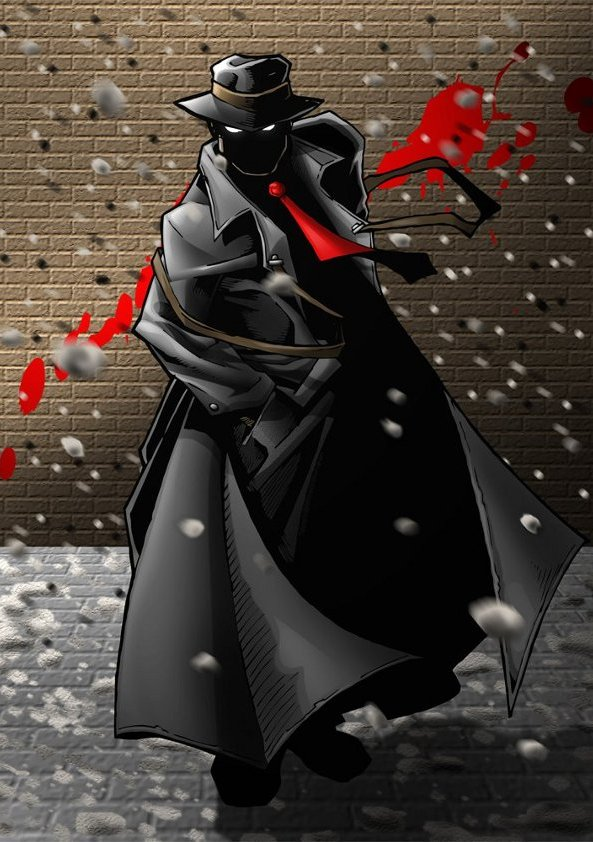
\includegraphics[width=\paperwidth,height=\paperheight]{images/cover}}
\begin{center}
    \color{white}\vspace*{\stretch{1}}

    \textbf{\fontsize{60}{72}\selectfont\itshape\thetitle}\vspace{1.5\baselineskip}

    \rule{0.5\textwidth}{3pt}\vspace{0.5\baselineskip}

    \textbf{\LARGE\theauthor}\vspace*{\stretch{1}}

    \large\theeditorial
\end{center}

\endinput

\newpage\pagecolor{white}

\frontmatter
\thispagestyle{empty}
\hbox{}\newpage
\thispagestyle{empty}
\vspace*{\stretch{1}}\noindent
\textbf{\titlename}\\
\authorname

\footnotesize

\bigskip\bigskip\noindent
\textbf{\copyright\ 2010--2011, \authorname}\\
\textbf{\copyright\ 2011, de la edición, \editorname}\\
Se otorga el permiso para copiar, publicar y/o distribuir libremente esta obra y/u obras derivadas de esta obra, ya sea total o parcialmente, por cualquier medio y con cualquier propósito sin ánimo de lucro, siempre y cuando esta nota se mantenga.\\
{\fontencoding{OT1}\fontfamily{cmr}\selectfont\url{http://creativecommons.org/licenses/by-nc-sa/3.0/es/}}

\normalsize

\noindent\ccbyncsaeu

\footnotesize

\bigskip\noindent
\textbf{Edición:} \editorname\\
Realizada íntegramente con \emph{software libre}, mediante el procesador \LaTeXe\\
\Letter\ {\fontencoding{OT1}\fontfamily{cmr}\selectfont\href{mailto:xoansampainho@gmail.com}{\nolinkurl{xoansampainho@gmail.com}}}\\
\Telefon\ \href{tel:+34620194971}{+34 620194971}

\bigskip\noindent
Impreso en la Red. \emph{Printed in Internet}

\normalsize

\endinput


\maketitle

\cleardoublepage
\raggedcolumns
\tableofcontents
\flushcolumns

\chapter{\prefacename\ \emph{\mdseries(Spin-off)}}
\cftchapterprecis{<<Canción triste>>, por \prefaceauthorname}\par
La noche era fea, ni más ni menos que todas las noches anteriores desde hace mucho tiempo. La Nube lo cubría todo, un manto sucio que arropaba Ernépolis~I y aplastaba con su peso los ánimos de todos los ciudadanos de la urbe. Bueno, quizá todos los ilustres que en esos momentos festejaban quién sabe qué bajo la gigantesca cúpula ni siquiera se habían percatado de que del cielo caía ceniza, suficiente tendrán con mirar las burbujas de sus copas de champán.

Y ahí estaba yo, a los pies de la enorme estructura de cristal, haciendo de niñera, el trabajo más emocionante que he hecho en las últimas semanas, la otra vez que me tocó hacer algo tan divertido fue cuando ayudé a la señora May a cambiar la bombilla de su hall, estaba sola desde que la abandonó el cabrón de su sobrino, justo cuando más falta le hacía\dots\ Pero bueno, para eso estamos nosotros: \textsc{Proteger y Servir}; ese es el lema que lleva escrito mi vehículo. Desde que los enmascarados, guardianes, justicieros\dots\ ¡superhéroes! decidieron proteger a los habitantes de Ernépolis~I, los policías solo hemos quedado para servir. 

Superhéroes\dots\ Unos tipos anónimos que pueden volar y a los que las balas les rebotan. Seguro que para ellos no es nada más que un pasatiempo, si yo tuviese ese poder también sería un héroe. Auténticos superhéroes fueron McClane, Walker, Romerales\dots\ A ellos no les rebotaban las balas y no dudaron ni un segundo en proteger a los inocentes, sin embargo casi nadie se acuerda de ellos\dots

Ahora somos un adorno, han recortado tanto la plantilla que llevo años sin compañero, y el coche ni siquiera tiene calefacción. Pelado de frío \emph{vigilando} una fiesta de pijos\dots\ Ya es hora de ir a por un café y unos donuts. 


\mainmatter
\addtocontents{toc}{\protect\vspace{0.5\cftbeforechapskip}\protect\begin{multicols}{2}}
\chapter{El fin}
\noindent
En ocasiones se preguntaba cómo pudo suceder algo así. Ocurrió muy deprisa, y no tuvo nada que ver con cómo lo había imaginado. Siempre supo que tendría que llegar ese momento, pero lo veía exteriorizado, como si él no estuviera allí. Llegó a pensar que ni siquiera se enteraría de ello. Nada más lejos de la realidad.

\bigskip\noindent
John Scream apuró el último trago de su copa y echó un vistazo a la sala de fiestas en la que se encontraba. Varias plantas comunicadas por escaleras imperiales, mucha vegetación a su alrededor, y todo ello cubierto por una cúpula de cristal. Como si estuvieran con eso aislados del mundo exterior.

Como si con eso no se viera la Nube.

A pesar de todo reconoció los esfuerzos de su anfitriona, Ellen Gorgon, para preparar una agradable velada a los invitados, algunos muy poderosos y que podían ofrecer respaldo a la emergente carrera electoral de Gorgon. Miró a Aryn, con aquel vestido de una pieza que a él tanto le gustaba, y trató de relajarse por ella. Últimamente su relación estaba en la cuerda floja y no le pasaba desapercibido el motivo. Tener una doble vida y ocultárselo no era la mejor estrategia para afianzarla, claro, pero tenía miedo. Miedo de que Aryn no aprobara su cruzada particular. De que su vida corriera peligro si conocía su secreto. De que pasaran ambas cosas.

~---¿Ocurre algo, John? ~---la voz de Aryn flotaba como el metal bruñido por la bulliciosa sala~---. Te veo pensativo.

La reflexión fue tan cruda que Scream la soltó tal cual llegó a su cabeza, sin depurarla siquiera.

~---Lamento haber estado ausente tanto tiempo.

~---Lo sé ~---ella se limitó a mirarle con sus ojos cristalinos, relajantes como un campo de trigo al atardecer.

~---He tenido demasiados viajes al exterior. Me gustaría tanto no tener que salir tan a menudo\dots\ tener una vida más estable.

~---Pero tú eres el mejor piloto espacial, John. Te necesitan. Y estoy orgullosa de tu trabajo.

Scream se preguntó si no estaría hablando con doble sentido. Si no sabría que a veces, muchas veces, ocultaba la verdad. Por una buena causa, pero no dejaba de ser una mentira, veneno que se interponía entre ellos dos. Y sabía que el tono comprensivo de sus palabras revelaba una súplica. Casi podía oírla, alzándose sobre todas las voces de la sala. Déjame saberlo, por favor, John. Dime quién eres en realidad. Pero no podía contarlo. No entonces. No en aquel momento, en aquel lugar.

~---Me alegro, cariño ~---se limitó a decir. Su voz sonó tan falsa como cuando la forzaba para que no le identificaran sus enemigos.

Apesadumbrado, pensó en acercarse a tomar otra copa, pero desistió cuando observó, no sin cierta estupefacción, que la propia anfitriona, Ellen Gorgon, se acercaba hacia ellos. Era una mujer joven que sabía vestir con elegancia. Su belleza, sin embargo, quedaba mutilada por culpa de su injerto. Scream no pudo evitar mirar.

~---Espero que estén pasándoselo bien ~---dijo con su voz melosa. Scream se dio cuenta de que llevaba la mano a la espalda. Se preguntó si a ella le repugnaría tanto como a los demás.

~---Una fiesta magnífica, señorita Gorgon.

~---Llámeme Ellen, John. No sea tan formal.

~---¿Qué fue lo que le pasó en el brazo, Ellen? ~---preguntó Aryn.

Scream miró sorprendido a su novia. Era la primera vez que veía a alguien formular abiertamente aquella pregunta. Se contaba, se rumoreaba\dots\ pero nadie lo sabía con certeza.

Gorgon enseñó lentamente el brazo oculto, como si no tuviera claro que se refiriera a él. Se trataba de un apéndice delgado y gris que acababa en tres dedos largos y tan finos que parecían carecer de huesos.

~---Fue un atentado, señorita Life. En una visita de rutina a mis factorías coloniales trataron de acabar conmigo con explosivos de corto alcance. Salvé la vida, pero mi brazo tuvo que ser tratado de urgencia con tecnología alienígena. Éste fue el resultado. Desagradable pero práctico.

Escondió otra vez la mano, como si el mundo no debiera verla por demasiado tiempo a la luz.

~---Dígame, Ellen ~---preguntó Scream~---, ¿a qué se debe invitarnos a nosotros a su fiesta?

~---No todo son estrategias electorales en mi vida, John. Deseaba conocer al hombre del cual hablan mis comandantes con tanta admiración. Siempre pensé que sería un magnífico piloto de pruebas para mis naves espaciales.

~---Agradezco el cumplido, pero ya sabe que vuelo por libre.

~---Por supuesto, pero por favor considere\dots\ ~---de repente llamaron a Gorgon por línea privada~---. Discúlpenme un momento ~---se retiró a un lado.

~---¿Tú que crees, Aryn? ~---preguntó Scream intrigado~---. ¿Crees que acabará gobernando Ernépolis~I?

~---Parece que oportunidades no le faltan. Controla la mayor parte del mercado espacial, y es cierto que desde que ella está aquí las exportaciones a Talópolis~IV, Ernépolis~II y las otras ciudades de los alrededores no han dejado de crecer.

~---Igual que la Nube ~---Scream miró al cielo grisáceo.

~---Es verdad que deberían poner solución a\dots\ ~---Aryn se tambaleó un momento.

~---¿Estás bien? ~---preguntó Scream preocupado.

~---Sí\dots\ sólo ha sido un mareo. Pero estoy un poco\dots\ indispuesta\dots

Al poco se unió Gorgon de nuevo a la conversación.

~---Ya estoy con ustedes. Vaya, señorita Life ~---dijo mirando a Aryn~---, no tiene buen aspecto.

~---Es posible que algo\dots\ me haya sentado mal.

~---Si quiere puedo mandar a un coche que la lleve a casa.

~---No se preocupe ~---dijo Scream cortante~---, ya la llevo yo.

~---Lamento que la fiesta haya sido así. Por desgracia yo también debo irme. Me han informado que hay intrusos en mi factoría más importante. Seguramente quieren mis últimos avances en el mercado espacial.

~---¿Intrusos? ~---dijo Scream lamentándose. Ni siquiera en su noche libre se podría relajar.

~---Así es. Los guardias del interior no responden, pero desde el exterior no han oído ruido alguno. Parece obra de un profesional.

Scream pensó que Gorgon estaba seguramente en lo cierto. Si la intuición no le fallaba se trataba de su peor enemigo, Silenciador. Un letal y sigiloso asesino a sueldo. Tenía que detenerlo cuanto antes.

~---Tengo que informar a mis socios yo también, Ellen. Si no es mucha molestia, agradeceré ese coche que nos ofrecía.

~---En absoluto. Ahora mismo estarán aquí. Si me disculpan\dots

En medio del bullicio Scream se sintió otra vez solo. Incluso al lado de Aryn, mientras no pudiera contar la verdad, ella sería una extraña más. Pronto, se dijo. Pronto tendría que hacerlo. Si no, era muy probable que su relación se acabara para siempre.

~---Aryn, ¿estás mejor?

~---Sí\dots\ ~---dijo ella llevándose la mano a la frente~--- pero aún estoy débil\dots

Al cabo de un rato uno de los camareros de Gorgon les hizo señas para que le siguieran. Tuvo que admitir que Ellen Gorgon era eficiente.

Dejaron atrás la fiesta, el bullicio, el lugar al que en el fondo nunca habían pertenecido, y volvieron otra vez al exterior, donde un vehículo deslizante les esperaba. La Nube estaba calmada aquella noche, y no parecía que fuera a amenazar con polución baja ni lluvia de ceniza, pero nunca se sabía. El clima de Ernépolis~I era tan variable que ya nadie hacía caso de las previsiones meteorológicas.

Dejó a Aryn en el coche y buscó un callejón apartado. Por lo menos en aquel sentido no podía quejarse de la ciudad, pensó. Cuando lo encontró sacó de su bolsillo la gema, nítida y brillante, y la agarró con fuerza. Nunca se acostumbró a la transformación, nunca dejó de sentir el dolor inicial que laceraba su cuerpo como si lo estuviera retorciendo y moldeando. Cuando al fin acabó, se miró las manos. Podía haberse transformado miles de veces desde que tenía la gema, pero no podía eliminar aquel acto reflejo. Estaban, como todo su cuerpo, cubiertas de un campo de fuerza opaco que ocultaba su identidad. Ahora, lo sabía, era él. Era quien debía, quien quería ser.

El héroe conocido en Ernépolis~I como Reflector.

Se concentró y se elevó poco a poco hasta estar casi a la altura de la Nube, no sólo para tener una panorámica de su objetivo, sino para alejar toda sospecha de que Reflector fuera en realidad uno de los invitados de la fiesta de Ellen Gorgon. Miró a lo lejos, por encima de los edificios grises aunque vivos de Ernépolis~I, y distinguió la enorme fábrica que Gorgon había mencionado. Dirigió el rumbo hacia allí, su silueta recortada por la Nube, los paseantes nocturnos señalando hacia el cielo, hacia aquel protector que algunos pensaban era una criatura salvadora de otro mundo, algunos pensaban era una amenaza, pero todos sabían era único y especial.

Al fin llegó a la entrada de la fábrica, un enorme bastión parecido a un palacio industrial en el que Gorgon pasaba la mayor parte de su tiempo empresarial diseñando en persona los nuevos modelos de naves espaciales que luego inundarían el mercado. Era buena, pensó mientras echaba un vistazo alrededor, pero no era piloto, y eso se notaba en sus diseños, demasiado poco arriesgados, demasiado aerodinámicos. No tardó en encontrar un par de guardias tirados en el suelo. Muertos. Usando sus poderes los sondeó con rayos X. Les habían disparado, pero no se trataba de heridas de bala. Era él. Su peor enemigo.

Entró levitando, teniendo cuidado de no hacer ruido alguno. Sabía que Silenciador podía esconderse, y aprovechándose de que su arma no hacía ruido, ni siquiera al disparar, acabar con aquello antes siquiera de que empezara. Detectó un levísimo olor a ozono, el único rastro de la presencia de su arma. Como mínimo había estado allí. Sin embargo no dejaba de tener la sensación de que estaba en una trampa. Una sala grande, llena de sombras, ideal para una emboscada. Absoluta quietud. Como si el aviso hubiera sido una falsa alarma. Al fondo encontró los cuerpos de más guardias. Muertos de igual manera. Y aquel olor\dots\ más fuerte\dots

Reflector apenas tuvo tiempo de apartarse antes de que una descarga a quemarropa lo fundiera. Su campo de fuerza podía reflejar tanto los golpes como los disparos de las armas convencionales, pero en el caso del arma de Silenciador, única en el Universo, sólo podía, a duras penas, resistir impactos lejanos.

~---Tu compasión será tu perdición tarde o temprano ~---dijo su enemigo a su espalda. Reflector se dio la vuelta y le vio claramente. Con sus ropas informales, casi anodinas, y su arma compuesta de varios tubos de metal, el cañón humeando aún. Su rostro descubierto, los ojos que tantas veces antes había visto. Refulgiendo de odio. Reflector le envidió. Envidió que un cobarde como aquel, capaz de asesinar por la espalda sin dudarlo, pudiera ir por la vida con el rostro descubierto siendo su verdadero nombre un misterio, mientras que él, que peleaba por la justicia, tenía que ocultarse de todo y de todos.

Incluso de Aryn.

~---Se acabó, Silenciador. Tira el arma. No lo empeores.

~---No seas estúpido, idiota disfrazado. Acaba de empezar. No les quería a ellos. Te quiero a ti.

Reflector comprendió que era una trampa. Pero no dejaba de entender por qué. Sin embargo, una vez en la telaraña, no le quedaba más opción que luchar. Miró con atención los cañones del arma de su enemigo. De vez en cuando giraban entre sí para encajarse alrededor del principal, poseyendo los demás funciones altamente diferenciadas. Su supervivencia dependería de adelantarse a ellos.

~---No tienes escapatoria. Saben que estás aquí.

~---Entonces acabemos cuanto antes.

El revólver futurista giró y un cañón con estrías se deslizó en la ranura principal. Al momento una red electrificada cayó sobre Reflector. Descargó toda la energía del traje en absorber su energía, para acto seguido agarrar la red y lanzarla contra su enemigo. Silenciador la interceptó y la apartó sin esfuerzo.

~---Crees que me voy a dejar atrapar por mi propia\dots

Cuando Silenciador miró al frente se encontró con que tenía a Reflector volando en su dirección a toda velocidad. Demasiado cerca para cambiar la modalidad del arma, recibió un tremendo puñetazo que le alejó varios metros hacia atrás.

~---No, bocazas, sólo esperaba distraerte ~---respondió Reflector.

Silenciador se incorporó y cambió el arma a rayo de baja energía pero alta velocidad. Comenzó a disparar en todas direcciones, esquivando Reflector con dificultad sus impactos. Volando de un lado para otro, trató de acercarse a su enemigo, pero sabía que el mismo truco no le serviría. Aun así lo intentó, pero cuando se acercó Silenciador fue más rápido. Ajustó el arma a la modalidad campo de energía y un haz lo protegió, chocando Reflector contra él y cayendo al suelo. Se levantó al momento antes de que su enemigo tuviera tiempo de lanzarle una descarga letal.

De repente las luces de la fábrica se iluminaron.

En las plataformas superiores aparecieron un montón de hombres armados que apuntaban a ambos contendientes. Tanto Reflector como Silenciador pararon y esperaron. Los recién llegados no suponían amenaza para ninguno de los dos.

Ellen Gorgon apareció rodeada de varios de aquellos soldados. Desde donde estaban apenas era poco más que un punto lejano, sin embargo su voz sonaba poderosa en toda la estancia. Parecía, al contrario que en la sala de fiestas, estar en su elemento.

~---Agradezco su colaboración, Reflector. Al parecer la ciudad está a salvo con su presencia.

~---No era necesario que viniera hasta aquí ~---dijo tratando de forzar la voz incluso más de lo habitual. No solía encontrarse con las mismas personas en ambas identidades.

~---Comprenderá que haya hecho lo contrario. Al fin y al cabo tenía que asegurarme de que el plan funcionaba.

Reflector empezó a tener la vaga sensación de que el suelo se hundía bajo sus pies, y que por mucho que supiera volar no podría evitar hundirse a su vez.

~---¿De qué está hablando?

~---Hablo del plan para acabar con usted de una vez por todas\dots\ Capitán Scream.

Aunque el campo de fuerza impedía ver su rostro, sabía que todos los presentes le imaginaban vulnerable y expuesto. Pero aún era un héroe. Aún podía tratar de hacer algo.

~---No sé de qué habla, criatura terrestre. Yo no soy como ustedes.

~---Muy al contrario, Capitán. Es muy humano, aunque físicamente sea más que uno. Por eso hemos podido tenderle esta trampa. Durante mucho tiempo Reflector ha frustrado, sin saberlo, mis intentos por hacerme con esta ciudad, por muchos obstáculos que he puesto en su camino, por muchas veces que se haya enfrentado a mi leal soldado ~---miró a Silenciador~---. De modo que opté por algo distinto. Las elecciones están en juego y no podía dejar a una amenaza como él suelta para discutir mi control, menos aún cuando sea del dominio público.

\rquoti Mis sospechas siempre cayeron en alguien que hubiera viajado mucho. Los poderes de Reflector no eran de este mundo, pero bien podían ser de otros. Sin embargo su carácter único lo alejaba de los lugares de habitual comercio y situaba su fuente en algún planeta o bien abandonado, o bien en proceso de formación. Examiné miles de historiales de vuelos espaciales, Capitán Scream. No fue fácil. Había muchos sospechosos, y aunque usted fuera uno de los principales tenía que estar completamente segura. Y lo estuve cuando al fin comprobé que hace muchos años su nave desapareció en una remota región apenas explorada. Encontré un planeta donde había un mineral\dots\ un mineral con efectos parecidos a los poderes de Reflector. Sin embargo fui incapaz de procesarlo. Tal vez si me dice cómo lo hizo le deje vivir.

Reflector sabía que la respuesta no iba a dejar satisfecha a Gorgon. Fue el último habitante del planeta quien, antes de morir, lo hizo para él, llevándose el secreto a la tumba. No podía perder ni un segundo. Era en aquel momento o nunca, mientras Gorgon soltaba su interminable charla acerca de lo magnífica que era y de cómo le había derrotado. Voló lo más rápido que pudo, dejando atrás la mayoría de las balas, rebotando las demás, hasta estar casi a la altura de la que siempre, sin saberlo, había sido su mortal enemiga. Ya casi estaba a su altura y dispuesto a noquearla de un puñetazo cuando, a un metro de distancia, se detuvo. Gorgon llevaba una pistola en su mano alienígena, y con ella apuntaba a Aryn, casi desmayada.

~---Atrás, Scream. Muy lentamente, vuele hacia atrás, o Aryn Life morirá.

Sin otra alternativa, hizo lo que le mandaron. La cosa se ponía cada vez peor.

~---De modo que fue en la fiesta\dots\ la bebida que ella tomó.

~---Todo estaba cuidadosamente calculado, Capitán Scream. ¿Me cree tan estúpida de presentarme aquí expuesta con un montón de soldados armados que no tienen nada que hacer contra usted? No, ellos están aquí sólo para nuestra coartada. Atacaban una de mis factorías, y el causante de hecho era el héroe conocido como Reflector\dots\ ya me deshice de otros héroes antes, y ahora le toca a usted. Descienda y vuelva a su estado normal\dots\ no repetiré las consecuencias de no obedecer.

~---No creerán que ataqué su factoría.

~---Es posible. Pero tampoco me desmentirán.

Incapaz de hacer nada en dicha situación, Reflector hizo lo que le ordenaban. Aterrizó y guardó de nuevo la gema en su bolsillo, cesando la transformación delante de todos los presentes. Aquel momento, comprendió, fue el fin definitivo de Reflector. A partir de aquel instante sólo era John Scream. Sólo un hombre.

~---Suéltela, Gorgon.

~---Como desees.

Gorgon empujó a Aryn fuera de la plataforma, cayendo a toda velocidad a la planta principal. Estaba tan mareada que ni siquiera gritó. Scream sabía que había suficiente altura para que se matara, por lo que trató de correr hacia ella, con todas sus fuerzas para acelerar la transformación. Aquel era el momento crucial. Sabía que podía muy fácilmente destruir para siempre la gema por forzarla demasiado, pero la vida de Aryn bien lo merecía.

El campo de fuerza envolvió otra vez su cuerpo, y de correr pasó a volar en cuestión de segundos, elevándose cada vez más. Ya casi podía llegar a su mano, extendiendo la suya desesperado, apenas reparando en los ojos de Aryn, sólo mirando aquella mano que caía como si fuera ella quien estuviera intentando salvarle a él y no al revés\dots

Recibió la descarga justo en aquel momento. Una andanada letal proveniente del arma de Silenciador. Ni el más mínimo ruido. Como una gota de agua desviada por el viento, cayó sin fuerzas de tipo alguno.

Lo último que oyó fue el chasquido del cuello de Aryn al romperse contra el frío suelo de la factoría.

Gorgon bajó, arma en mano, e ignorando el cuerpo de Aryn Life se acercó hacia Scream. Ningún campo de fuerza le protegía. Sólo era John Scream.

~---Está muerto ~---dijo con calma mirando a Silenciador~---. No debías matarlo, idiota. Has agotado el poder de la gema. Ya no me sirve de nada, ni él ni su objeto.

~---¿Qué sugiere que hagamos con él? ~---preguntó lacónicamente Silenciador.

~---Tiradlo a los bajos fondos. A la chica llevadla a los callejones cercanos a la fiesta. Vosotros dos ~---dijo señalando a dos de los guardias~--- vestiros de paisano y fingid que la habéis matado allí en un atraco. Vamos ~---dijo impaciente. Cuando los hombres se fueron Gorgon hizo una llamada~---. Sí, con el Jefe Wolf. Soy yo. Cumpla con su parte. Cuando sus hombres los detengan, ya sabe qué hacer. Sí, mientras huyen. De acuerdo. No me falle.

Ellen Gorgon se dio la vuelta y, satisfecha, miró a sus hombres mientras con la mano alienígena guardaba su arma.

~---Caballeros ~---dijo con voz solemne~--- la era de los héroes ha llegado a su fin.

\endinput


\chapter{El principio}
El fin. De todo lo que alguna vez fue su vida, su aliento. Esperanzas desaparecidas. Aquel que debió ser un defensor, indefenso. Y sin embargo, tal vez un nuevo comienzo estaba esperando para darse a conocer\dots

\fancyparbreak
Silenciosamente, un vehículo deslizante llegó a la zona sur de Ernépolis~I, una de las más deprimidas de la ciudad, con la intención de librarse de una carga que debía desaparecer. Se detuvo frente a un callejón mientras su también silencioso ocupante descendía y abría la compuerta trasera. Miró al cielo y maldijo por lo bajo, pues se preparaba una lluvia de ceniza. Deseoso de que no le atrapara en plena faena, cogió el cuerpo y lo llevó al fondo del callejón oscuro. Con un poco de suerte, pensó, nunca lo encontrarían, aunque sabía que Gorgon no se sentiría satisfecha con eso. Ella querría que lo encontraran. Él no. Era la muerte que le correspondía a su enemigo. En nada heroica, en nada épica. En un callejón. Perdido, abandonado de todos. Sin identidad. Sin poderes, sin nada que acreditase lo que había hecho por los demás. Anónimo. Despreciado, incluso rechazado.

Le miró un momento fugazmente. Aquel era el gran Reflector, el que había frustrado sus planes siempre, incluso antes de que tuviera que convertirse en soldado de Ellen Gorgon. Un muñeco roto. Del mismo modo que tarde o temprano él acabaría en otro callejón oscuro, igualmente olvidado, sus grandes peleas polvo y ceniza. Una parte de él se alegraba de haber acabado con su enemigo. Otra deseaba el retorno de la danza sin fin. Reconcilió ambas partes y subió al vehículo, pero antes, dedicó un momento a mirar su arma. Recordó cuando tuvo que matar a aquel que la construyó para él. Para que fuera única, irrepetible. Lo mismo pasaba con la marioneta sin hilos que acababa de dejar en el callejón. Se marchó reflexionando que ya habría otros Reflectores en el mundo.

O tal vez no.

Finalmente la ceniza empezó a caer. Con lentitud, como si estuviera siendo esparcida desde los balcones, con más fuerza al final. Sin embargo parecía que los desagües funcionaban bien. Aquella noche el nivel no subiría de un centímetro. Cuando se atascaban, la capa de ceniza podía ser de diez. Un motivo por el que la mayoría de los ciudadanos que podían permitírselo no vivían a nivel de calle.

La gema, que aún permanecía en el bolsillo de John Scream, brilló. Con un fulgor que no había tenido nunca antes y que no volvería a tener. En un último esfuerzo reunió todo su poder para, con mucho tiempo y paciencia, curar las heridas mortales de su portador. Sin testigos, sin nadie que pudiera apreciar el milagro, realizó su tarea y su luz se extinguió definitivamente para no volver a brillar jamás. Reflector había dado su vida al salvar a John Scream, la última víctima inocente.

Scream movió un dedo. Con mucha dificultad, como si no fuera suyo. Apenas un palmo. Nada perceptible ni por una rata. Estaba vivo. No debía estarlo, pero lo estaba. No era el final. No al menos de momento. Estuvo mucho, muchísimo tiempo tumbado sin poder recuperar la posición vertical. La gema le había salvado con su último aliento. No lo había visto, pero lo sabía. Se acabó.

Sus ideales, sus creencias, sueños rotos. Derrotado. El fin de Reflector. El fin de John Scream tal y como se le conocía. Debía huir. Esconderse de sus enemigos. Ya nada podía hacer contra ellos más que observar desde la retaguardia. Los héroes habían perdido. No sólo él, sino también los otros que Gorgon decía haber aniquilado. La creía capaz de ello. Parecía tener mucho tiempo, mucha paciencia, y sobre todo recursos y voluntad para utilizarlos. Empezó a sospechar que el atentado que le costó la mano en realidad nunca fue tal.

Como un símbolo de la vida que perdió, contempló la gema apagada y sin brillo. Los rescoldos de un fuego que no volvería a arder. Se incorporó y corrió a refugiarse de aquella mugre que caía del cielo.

A partir de entonces las calles se convirtieron en su hogar. Sabía que no podía volver a su anterior vida. Aun sin Aryn, aun sin Reflector, no podía volver a ser John Scream. No podía volver a pilotar. Si es que quería sobrevivir, tenía que convertirse en alguien completamente distinto de quien fue. Un vagabundo era una opción tan buena como cualquier otra. Salvo la propia Gorgon, dudaba que algún otro de los que habían presenciado su amarga derrota recordara su rostro. Por si acaso se dejó crecer barba, aunque suponía que su aspecto sucio y su ropa hecha jirones bastarían para hacer el resto.

Él, que había surcado los cielos, se convirtió de repente en otra de las motas imperceptibles que desde arriba apenas alcanzaba a divisar. En cierto modo lo prefirió así. Desaparecer. No era tan malo, y la opinión pública siempre le recordaría como un héroe. Los titulares así los remarcaron. \textsc{¿Dónde está Reflector?} No se asoció la desaparición de Reflector con la de John Scream, al fin y al cabo Reflector era una figura de gran relevancia, y John Scream sólo sería una reseña al final de la última holopágina, y eso si alguien llegaba a echarle realmente de menos, dado que al ser piloto no le eran desconocidas las prolongadas ausencias.

Ni siquiera se le relacionó con la muerte de Aryn Life. Scream esperaba malevolencia por parte de su enemiga, la ironía de cargar con el crimen a aquel que intentó salvarla, pero no fue así. Fue lista. No quiso llamar la atención. Con el tiempo todo se olvidó, la gente empezó a dejar de preguntarse dónde estaba su héroe, y el asunto fue dejado de lado. Simplemente pasó, como las rachas de viento.

Pero la ciudad necesitaba gente como Reflector. John Scream lo sabía. Con su ausencia, Ellen Gorgon se convirtió en la dueña del crimen organizado. Usando sus influencias controló media ciudad, y una vez lo consiguió ganó las elecciones, convirtiéndose también en dueña de la otra mitad. La corrupción inundó Ernépolis~I. Pocos eran los policías que desafiaban las normas, y la mayor parte de ellos acababa formando parte de las naves espaciales al ser echados sus cuerpos en los tanques de fundición de las factorías de Gorgon. Algunos héroes surgieron, pero tan pronto como aparecían volvían a desaparecer, bien chantajeados, bien eliminados por el eficiente brazo de Gorgon y nuevo colaborador de la ley, el reformado Silenciador, pues su deuda con la ley había sido pagada con las influencias de Gorgon.

Los jueces, la ley, las factorías, el gobierno. El ascenso de Gorgon era imparable. Sólo había que mirar al cielo. La Nube era mucho más densa y oscura. Lo que en su día fue gris pero de colores vivos se convirtió en negrura, una ciudad donde los extranjeros no querían parar, donde la noche duraba veinticuatro horas. Una ciudad que cada vez exportaba más, y por tanto donde nadie quería meter la narices. Una ciudad que empezó a prescindir del trámite de las elecciones.

Retazos de todas estas noticias llegaban a los oídos de John Scream, que no hacía más que seguir mirando en qué se había convertido la ciudad que trató de defender con todos sus esfuerzos. La justicia, la venganza, el poder perdido, todo aquello bullía por sus venas, entremezclándose, clamando por salir. Pero John Scream no lo dejaba salir. Sólo era un hombre, pensaba. Nada podía hacer. Sólo observar\dots\ y lamentarse en silencio.

Y así pasaron los años. Y Ernépolis~I se hizo más grande, más poderosa, más rica, pero no para todos por igual. De cara al mundo era una gran exportadora. De cara a sí misma era un vertedero de hombres. Un reino de polución y ceniza. Donde no hacía falta escarbar para encontrar la podredumbre de la raza humana.

Donde sin embargo era necesario hacerlo si se quería encontrar a los que en su día fueron un ejemplo para los demás.

\parbreak
Una noche, tiempo después, Scream estaba en un callejón, en plena lluvia gris, buscando comida, cuando vio al fondo del mismo, recortada por la luz de los vehículos deslizantes, una silueta de un hombre con gabardina y sombrero. No parecía humano, y sin embargo nada indicaba lo contrario. Apartó la mirada un momento y desapareció. Nada. Como si nunca hubiera estado. Pero estaba. No habían pasado tantos años como para haberse atrofiado su instinto. A veces deseaba que fuera así, pero no había visto, al menos aún, su deseo cumplido.

\emph{Tú eres él.}

La voz se propagó por las reverberantes paredes del callejón. Scream se olvidó de la comida y trató de escudriñar sin éxito el lugar. La oscuridad y las sombras eran aliadas de aquel que le acosaba.

~---Descúbrete ~---dijo sin más.

\emph{No trabajo para ella, si es eso lo que te preocupa. Sé por lo que has pasado, John. Sé lo que es dejarse llevar por los demonios. Pero tú los has dominado. Contenido, al menos.}

~---¿Quién eres y cómo sabes mi nombre?

La silueta apareció como si no se hubiera movido y se acercó a Scream lentamente.

~---Sé tu nombre porque te he estado observando mucho tiempo\dots\ Reflector.

Scream se acercó a la silueta y vio a su interlocutor. Bajo la gabardina se ocultaba un rostro anciano pero vigoroso, el semblante de alguien que parecía haber acumulado gran experiencia en batallas pasadas. Scream se sintió como si estuviera frente a una versión distorsionada de sí mismo de haber sido otras las circunstancias.

~---Reflector murió hace años. Sólo queda John Scream.

~---Lo sé, John. Del mismo modo que en mi caso sólo queda Starr Miles.

Scream le miró y se fijó en él. Como si de repente una parte del pasado volviera para atormentarle.

~---Tú\dots\ yo te conocí. Tú fuiste como yo. Tú tenías otra identidad. Pero no soy capaz de identificar quién eras.

~---Eso ya no es importante, John. Como tú, yo también perdí esa identidad. Siempre supiste que tus poderes sólo te traerían desdicha. Quizás incluso intuiste un trágico final, para culminar con la muerte, solo, perdido y sin nada a lo que aferrarte. Pero no imaginaste que hubiera un después. Los comics que leías cuando eras pequeño no hablaban de eso. Esa es la infortunada existencia que nos tocó vivir. Tal vez hubiera sido mejor que hubiéramos muerto, como le pasó a otros muchos héroes. Pero somos supervivientes, y tenemos una obligación. No sólo para con nosotros mismos, también con la ciudad que nos prometimos en silencio defender.

~---Pero sólo somos hombres. Nada queda ya de lo que fuimos.

~---Un hombre ~---sentenció Miles~--- puede ser suficiente. Fuiste derrotado por alguien que no tenía poder alguno, que no era más que humana. Los poderes no son nada sin voluntad, John. La voluntad es más fuerte que todos los rayos, todos los puñetazos, todas las armas del mundo.

~---Es muy bonito todo tu discurso, Starr Miles. Pero no sé qué podemos hacer ahora, salvo fundar superhéroes anónimos y hacer un par de asambleas al mes ~---dijo Scream con chispeante amargura.

~---Es mucho lo que podemos hacer aún. Hace años yo pensé como tú. Yo tuve mi propia Ellen Gorgon, y tampoco salí bien parado. Como tú no vi esperanza alguna, pero pronto comprendí que debía hacer algo. Juré que mientras viviera protegería mi ciudad. Estoy en puertas de cumplir ese juramento. Ha sido duro, John. No es tan fácil como cuando se tienen asombrosos poderes, pero es posible marcar la diferencia. Hacen falta muchos años de paciencia, y nuestras hazañas no serán el capítulo de ningún libro de historia. Nadie nos lo agradecerá. Es posible que incluso nos teman. Pero no por eso debemos dejar de intentarlo.

~---¿A qué te refieres?

~---Me refiero a los Caídos.

John Scream miró de reojo a su interlocutor. Starr Miles captó su incredulidad.

~---Te preguntas si estoy loco. Si sólo soy un viejo charlatán que ya ha visto pasar sus momentos de gloria y ahora se aferra a un pasado que es como la ceniza que cubre el suelo ahora. Sólo polvo.

~---Digamos que me intriga lo que tengas que decirme.

~---Unirnos, John. A lo largo de los años he hablado con más gente como tú. Aquellos que fueron héroes, que defendieron ésta y otras ciudades, y que luego desaparecieron en extrañas circunstancias. En mi vida civil yo era detective. De ese modo me aproveché de aquello que siempre nos empeñamos en dejar de lado en nuestras actividades como protectores para encontrar a otros como nosotros. Ha sido, y sigue siendo, una búsqueda agotadora. Sabemos escondernos bien. Pero ha dado sus frutos. Aunque sólo hombres somos, juntos seremos mucho más que eso. Los años han pasado, y ha llegado el momento de surgir. De enfrentarnos con Ellen Gorgon y destronarla.

~---Ellen Gorgon ~---dijo Scream con furia~---. La mataría de poder hacerlo.

Starr Miles se acercó hacia él y le dio un potente puñetazo. Scream tuvo que usar ambas manos para apoyarse contra el suelo polvoriento.

~---No eres un asesino, así que no finjas comportarte como tal; por lo menos no a mí. Sé lo que hicieron. Sé que mataron a la persona que más querías en el mundo. Siempre lo hacen, y nuestro deber es ser mejor que ellos. Puede ocurrir que, por defensa propia, acaben muertos. Es algo que todos los que hemos sido héroes hemos pensado alguna vez, si no nos ha ocurrido de hecho. Pero matarles deliberadamente es un deliberado asesinato.

John Scream se levantó. Contra lo previsto por Miles, nada de furia había en sus ojos. Sabía que tenía razón. Por mucho que odiara reconocerlo, estaba en lo cierto.

~---¿Y cuál es tu plan? ¿Ser un ejército? ¿Derrotarles por superioridad numérica? No creo que haya tantos héroes caídos como para eso.

~---No tiene sentido atacarles cara a cara. Nuestra derrota sería ineludible. Tenemos que ser conscientes de nuestros medios. Si nos disparan sangramos, si nos golpean caemos. Como has caído ahora. Pero podemos levantarnos, y volver más fuertes de lo que nos fuimos. Todos nosotros somos muy experimentados, y eso nos da una gran sabiduría conjunta. Nuestros conocimientos añadidos, de hecho, nos otorgan un gran potencial científico. Por otro lado estamos en todos los estratos de la sociedad, los mismos que Ellen Gorgon cree gobernar.

~---¿De cuántas personas estamos hablando?

~---Debo deducir que te unes al proyecto ~---dijo Miles con satisfacción.

~---No puedo negar que la idea me seduce.

~---Me alegra oír eso. Sin embargo, como tuvo que hacer Platón con sus discípulos, tendremos que trabajar duro. Primero debes hacerte a la idea de que ya no eres, ni volverás a ser jamás, Reflector. Después, te convertirás\dots\ en otra cosa.

~---La primera parte será más fácil de lo que crees ~---dijo Scream tras pensarlo un momento.

Starr Miles rió por lo bajo.

~---Eso, amigo mío, es lo que creen todos al principio.

\endinput


\chapter{Aprendizaje}
Mucho tiempo después, sólo recordó la ceniza en su boca, dispersa por todo el suelo, mientras su mano trataba de aferrar la mano de ella. Tanto que había perdido\dots\ tanto por ganar.

\fancyparbreak
Existen muchas cosas que formaron parte de los recuerdos de John Scream por aquel entonces. El día que se estrelló en un planeta perdido sin esperanza de volver a remontar el vuelo. Cuando conoció al ser que creó la gema para él. La noche que conoció a Aryn. Su primera pelea contra Silenciador. El terrible instante en que éste, por orden de Gorgon, le disparó por la espalda y le impidió salvar a Aryn.

Pero ningún recuerdo fue tan vivo como el día que Starr Miles le mostró el Aquerón, el cuartel general de Los Caídos.

Había miles de entradas por toda la ciudad. Miles de pasadizos escondidos en todas partes. Ocultos, impenetrables, bien vigilados, para que si alguno de ellos era fortuitamente descubierto no se supiera mucho más al respecto de dónde llevaba. Simplemente, si eso ocurría, se procedía a inutilizar dicha entrada y se cerraba para sustituirla por una nueva. La que ellos utilizaron estaba cerca del lugar donde Scream había vivido la mayor parte de su tiempo desde que estaba en la calle. Miles se aproximó a un segmento de pared en un callejón oscuro. No parecía tener nada de particular, y durante el rato que esperaron, por mucho que Scream lo observó, nada vio que le hubiera hecho sospechar que tras ese muro se escondiera nada distinto de un almacén de ratas. Al poco el arcaico ladrillo se deslizó y les dejó paso a una oscura sala.

~---Una de las primeras cosas que aprenderás será a reconocer esta clase de accesos ~---afirmó Miles.

La puerta se cerró tras ellos y una tenue luz iluminó el pasillo. Scream se sintió más como si estuviera entrando en una base perteneciente a alguno de sus viejos enemigos que como conociendo el que supuestamente iba a ser su nuevo hogar. Había por todas partes metros y metros de pasillos intrincados en los que se hubiera perdido con gran facilidad.

~---Disculpa si tardamos, John, pero mi intención era enseñarte el módulo principal.

John Scream se preguntó si la espera valdría la pena. No lo dudó cuando llegaron al fin.

Una enorme sala de más de diez pisos de altura se ofrecía a sus ojos, escondida de la ciudad bajo sus cimientos. En ella pudo ver múltiples departamentos acristalados donde toda clase de personas se estaban entrenando. Mientras andaba con Miles no pudo fijarse más que en detalles aislados por aquí y por allá: hombres luchando entre sí con los puños y otras armas nobles, salas donde poner a prueba el sigilo, laboratorio químico donde vagamente pudo distinguir cómo hacían pruebas de combustión de tela, departamento electrónico, donde parecían hacer pruebas de modulación de sonido. Al cabo de un rato se pararon frente a una compuerta.

~---Entra ~---le dijo Miles. Una luz de alarma se encendió en la cabeza de Scream.

~---¿Por qué no entras tú\dots?

El golpe le dejó inconsciente al momento.

Cuando despertó se encontraba desnudo en la misma habitación donde le habían obligado a entrar. No había nada más que él. Golpeó la compuerta. Nadie respondió. Hacía frío. Mucho frío. Pero Scream no protestó. No iba a dejarse humillar.

No mucho después llegó comida a través de un panel. La tomó hambriento. Otra vez el silencio, la nada. Al cabo de un tiempo sintió la terrible necesidad de vaciar sus intestinos. Aguantó cuanto pudo, pero al fin tuvo que rendirse a la evidencia. La humillación era completa. Una especie de brazo robot surgió de la pared y le devolvió parte de la dignidad perdida limpiando la habitación hasta dejarla de nuevo como al principio. De nuevo silencio. El sueño comenzó a invadirle y dedujo que era hora de dormir. Sin embargo no durmió. Estuvo tres días sin hacerlo hasta que el sueño le derrotó.

Al cabo de una semana le dieron ropa. Pasó un día entero sólo tratando de volver a entrar en calor. Estaba enfermo, pero sobreviviría. Se dedicó a entrenarse dentro de su celda, no sólo para ocupar el tiempo. Su propio instinto latente le obligaba a ello.

Finalmente, al cabo de otra semana, dos hombres entraron en la jaula. Le miraron de reojo y comenzaron a atacarle. Golpes cuidadosos, calculados, destinados a cercarle. Scream les observó. No estaban acostumbrados a atacar cara a cara. Se aprovecharía de ello. Trató de agarrar a uno por la muñeca para inmovilizarle, pero éste se soltó con un rápido movimiento de pinza y con la mano opuesta hizo aquello que Scream no había conseguido. Al mismo tiempo el otro le agarró del brazo libre y se lo colocó a la espalda. Estaba inutilizado.

O no.

De un cabezazo que le dolió tanto o más que a la víctima, Scream derribó a uno de sus atacantes mientras se zafó de la presa del otro. Se disponía a realizar otro ataque cuando la compuerta se abrió de nuevo. Era Starr Miles.

John Scream se olvidó de sus atacantes y se lanzó al cuello del viejo.

~---Valiente pero impulsivo ~---dijo Miles agarrando de la barbilla a Scream con fuerza. Scream sabía que si apretaba le haría puré~---. No pierdas el sentido, John. Eso será lo que ellos pretenden. Si no te pueden derrotar, entonces tratarán de volverte loco.

Soltó a Scream y éste cayó al suelo con estrépito.

~---Me siento orgulloso, John ~---dijo indicando a los dos hombres que les dejaran solos~---. Era una prueba muy dura ésta a la que te has sometido. Pensabas que lo habías perdido todo. Ahora sí. Para nosotros ya no tienes dignidad. Has caído lo más bajo posible.

Miles le sonrió.

~---Igual que esos hombres. Igual que yo.

Los siguientes días algunos de Los Caídos le enseñaron el arte de la defensa personal. Scream podía ver en todos ellos el halo de los que han sido héroes alguna vez. Ocasionalmente el propio Starr Miles le adiestraba en persona, y fiel a sus ideas de adoctrinamiento le daba lecciones verbales mientras peleaban, consejos que eran asimilados por Scream fácilmente a pesar de tener que estar concentrado en otra cosa mientras los escuchaba.

~---Nosotros no combatimos, John. Esto es sólo una medida preventiva. Podíamos combatir cuando teníamos poderes que respaldaban esa clase de actos. Ahora nuestro poder es otro.

~---¿En qué consiste nuestro poder ahora?

~---En la astucia, John. Somos como los magos que efectúan sus trucos en los burdeles del este de Ernépolis~I. Tenemos que jugar con la percepción del enemigo. Engañarle. Estos tiempos que nos han tocado vivir favorecen la estrategia. La Nube es más oscura que nunca, la ceniza cubre las calles. Callejones, sombras\dots\ todo a nuestra disposición. Son armas tan poderosas como las que antes teníamos.

~---¿Y en qué consistirá el engaño?

~---Sólo somos hombres, John. Pero para ellos seremos más que eso.

Cuando su entrenamiento de defensa personal terminó, Scream pasó a la siguiente fase: el silencio.

~---Recuerda, John ~---decía Miles observando a Scream en el laberinto donde debía poner a prueba su sigilo~--- que todo es una cuestión de paciencia. Para ser una sombra debes comportarte como tal. No te desplaces, deslízate. Aprovecha los ruidos de la ciudad, son parte de tus movimientos. No seas rítmico. Y cuando llegue el momento de presentarte, juega con los claroscuros. Que no vean tu rostro. Calla cuando esperan que hables, habla cuando esperan que calles. Desconciértales, pero no les subestimes.

Un sensor tocó a Scream y disparó las alarmas del laberinto. Al momento tuvo que ponerse a cubierto, pues sabía que los disparos efectuados por las defensas del laberinto, aunque no eran letales, eran extremadamente dolorosos. A duras penas lo consiguió.

~---Sobre todo, John, piensa que si engañas al enemigo, si le haces temerte, éste puede hasta a llegar a dudar si dispararte o no por puro miedo. Ese poder es mayor que cualquier arma que puedas empuñar.

Una vez el entrenamiento básico estuvo completado, por fin Miles comenzó con Scream la etapa clave para ser uno de Los Caídos. La comprensión de lo que estaban haciendo. Le dio una gabardina y un sombrero a medida y Scream se los puso. No parecían tener nada de especial.

Hasta que Miles dejó la habitación en penumbra.

La combinación de luz y oscuridad ensombreció su rostro, convirtiéndolo en indetectable para alguien que estaba lejos de él. Se miró en un espejo y su imagen le resultó perturbadora. Anónima, pero al mismo tiempo dotada de personalidad.

~---Esta es la primera parte del engaño, John. Todos nosotros vestimos igual. El complejo cometido, como ya sabes, es hacer creer que sólo somos uno. Por eso la ropa, no sólo por su aspecto ambiguo y protector. Cuando estés fuera no tendrás identidad, aunque pertenezcas a Los Caídos. Eso es lo que somos. Muchos hombres que actúan como uno que no existe. Sin nombre. Sin pasado. Como una plaga de hormigas. Imparables.

Se acercó a Scream y le dio un par de lentillas y una pastilla.

~---Las lentillas son para que todos tengamos el mismo color negro de ojos. Los ojos son cruciales. Deben expresar todo lo que nunca haríamos. Si los criminales ven odio en los ojos, ellos sentirán temor. Si por el contrario ven temor, sentirán odio. La debilidad de los demás es su fortaleza. Nosotros les haremos sentir lo que provocan.

~---¿Y la pastilla? ~---preguntó Scream.

~---Algunos de nosotros, desgraciadamente, moriremos. Esa pastilla fue creada para hacer desaparecer nuestros cuerpos en caso de que eso ocurra. Tenemos que darles la sensación de que la criatura a la que se enfrentan es inmortal, ajena a las leyes de la naturaleza. Trágatela.

Así lo hizo Scream.

~---Bien ~---dijo Miles satisfecho pero sin ocultar la dureza de sus palabras.

~---¿Qué hay de la ropa?

~---Llevó mucho tiempo, pero diseñamos un tejido que puede arder espontáneamente cuando nosotros queramos. Puede ser accionado por un compañero oculto en las cercanías, y en caso de emergencia podemos hacerlo nosotros desde la base, previa advertencia para evitar posibles accidentes. Del mismo modo todos los aparatos que puedas llevar serían consumidos por las llamas para quedar sólo una capa de ceniza.

~---Muy apropiado ~---comentó Scream~---. Ceniza no falta en Ernépolis~I.

~---Y lo más importante al respecto, John. Tardarás mucho, pero aprenderás a no exteriorizar el dolor. Nunca, jamás, debemos gritar. Sobre todo al morir. Eso es lo que ellos esperan. Librarse de la pesadilla atravesándola, disparándola, lanzándola agua hirviendo. El éxito de la idea depende de detalles cruciales como éste.

~---Lo recordaré.

~---Sí ~---comentó Miles~---, no me cabe duda que lo harás.

A partir de ese momento Scream comenzó el entrenamiento con otros miembros del grupo. Resultaba muy duro para él, que siempre había trabajado solo, coordinarse con otros ya no en ataques sino en movimientos. Al final comprendió que era como si estuviera en un gran escenario y fuera un actor más sobre él. Mientras los focos no le iluminaran no sería el protagonista, pero tenía que aprender a entrar en escena cuando fuera su turno. Cuando la sincronización era correcta, cosa que cada vez sucedía más a menudo, los resultados eran espectaculares.

~---Perfecto, John. Aprendes deprisa. Te nombraré director de un escuadrón.

Los escuadrones solían ser de cinco miembros, los cuales se conocían a la perfección. Todos ellos se movían de idéntica manera para hacer el engaño lo más creíble posible. Scream no tardó en simpatizar con ellos: James Sky, Charles Razorclaw, Frank Raid y Ellis Saw. Sabía que ya se conocieron en el pasado, pero el entrenamiento de Starr Miles resultó tan eficaz que ninguno de ellos fue capaz de imaginar qué fueron los otros en la era dorada de los héroes.

Nadie solía hablar de su etapa anterior. No había ninguna regla que lo prohibiera, pero parecía una especie de acuerdo silencioso entre los miembros de Los Caídos. Sin embargo las pocas veces que el tema surgía y alguien se atrevía a contar su secreto, Scream se sentía sorprendido por las tan diversas formas en que habían acabado la carrera heroica de aquellos que hablaban. Sin embargo el tema recurrente siempre era el mismo: Starr Miles.

~---He oído que él no fue un héroe sino un villano, y que se arrepintió de su conducta ~---comentaba Razorclaw.

~---Eso no es así ~---contradecía Saw~---. Dicen que era el Hacedor.

~---Yo también he oído eso ~---terciaba Sky~---. Y si no es él, ¿de dónde sacó todo esto?

Pero Scream callaba. Sabía que la paciencia de un hombre bien podía construir todo lo que les rodeaba. Su escuadrón subestimaba no a su líder, sino su capacidad conjunta. Sólo sumando los cuarteles secretos que muchos de ellos tuvieron en su momento el resultado era una fortaleza casi inexpugnable.

A lo que Scream al fin comenzó a comprender la delicada tarea que se habían impuesto. Debían parecer ya no como sus enemigos, peores aún que ellos. La policía les buscaría, pero la policía estaba corrupta. El Jefe Wolf, por orden de Gorgon, no cejaría hasta detener al extraño de la gabardina y sombrero. Pero ellos no estaban indefensos. Sky era policía. Razorclaw era abogado. Raid era profesor universitario. Saw trabajaba para Gorgon en persona. Tenían acceso a todos los niveles. Sin embargo él estaba fuera de la sociedad, y sabía que por eso era el jefe de su escuadrón. Tenía más tiempo para dirigirles, para perfeccionar su entrenamiento personal. Para asimilar el objetivo.

~---No deben creernos héroes ~---repetía Miles una y otra vez~---. Ellos no tienen escrúpulos a la hora de amenazar a los que nos importan. Con todo el dolor de nuestro corazón, tenemos que dar la sensación de ser peores criminales que ellos. Jamás deben sospechar que nos preocupan los inocentes, y de ese modo no los usarán para amenazarnos. No nos chantajearán con vidas ajenas, como te ocurrió a ti y a muchos de los que están aquí ahora. Hay veces que saldremos al exterior sólo para provocar miedo y pánico entre los transeúntes, llegando incluso a fingir que matamos alguno de ellos. Seremos erráticos. No sabrán qué queremos, si justicia, venganza, o controlar la ciudad.

La última fase introdujo los aparatos especiales. Moduladores de voz para que todas sonaran iguales. Hologramas de múltiples tipos, desde distorsionadores de imagen para aumentar las siluetas y las sombras hasta fieles reproductores de imagen real. Armas aturdidoras que parecían letales. Anuladores de fotones para provocar y manejar la oscuridad. Una tecnología sin igual extremadamente difícil de manejar con éxito.

~---Dentro de poco nos pareceremos a los Cazadores de Nocturnos de Talópolis~X ~---murmuró Raid para sí cogiendo los aparatos.

~---Vamos, tenemos que practicar. Hoy emboscada ~---dijo Scream en voz alta.

Con unos reflejos asombrosos, los miembros del escuadrón se pusieron en sus puestos. Todo funcionaba a la perfección entre ellos. Pero Scream no estaba satisfecho.

~---Tenemos que salir al exterior ~---dijo a Miles en cuanto pudo~---. Tenemos que conocer la ciudad.

~---Y así se hará ~---respondió Miles~---. El momento ha llegado. Poco a poco al principio, con más intensidad después, vamos a mostrarnos a Ernépolis~I.

Scream le miró fijamente y por primera vez notó un atisbo de temor en sus ojos. Nunca una palabra de Miles lo corroboró, pero supo que el entrenamiento, al fin, había finalizado.

\endinput


\chapter{Surgimiento}
Nunca pensó que llegaría a hacer algo así. Siempre creyó que cuando estuviera con otros héroes serían admirados. Valorados. Que su labor tendría recompensa. Pero al fin se dio cuenta de que su promesa de defender a los que más quería podía hacer que sintieran miedo de él y los suyos\dots

\fancyparbreak
Por primera vez en bastante tiempo volvía a caer aguaceniza en las calles oscuras de Ernépolis~I. La combinación de ambas lluvias provocaba una sustancia plastosa que permanecía por varios días en el suelo de la ciudad hasta que nuevas lluvias sólo de agua contribuían a reblandecer la mezcla. Era por eso que Roger Thunder suponía que aquella iba a ser una noche inútil. Allá en los Túneles, nadie sería tan estúpido como para deambular a dichas horas en mitad de una lluvia de aguaceniza. En ese sentido el negocio iba cada vez peor, y Thunder lo sabía. Tendría que empezar a plantearse mudarse de barrio si es que quería cumplir con la cuota monetaria semanal para su jefe. Si no lo hacía ya sabía lo que le tocaría: llamarían a los hombres de Wolf y éstos le meterían en la cárcel tras una interminable sucesión de torturas. Recordó una vez en que encontró a un excompañero de correrías que acabó así. Había huido, decía, en un descuido de sus captores. Su aspecto no parecía evidenciar tal cosa. Thunder supuso que las cárceles de la poli estaban tan llenas de tipos que habían intentado oponerse con la razón a Gorgon que bien podían soltar a un inepto más por la ciudad.

Sumido en sus pensamientos, de repente vio a lo lejos la silueta de una mujer corriendo para guarecerse bajo uno de tantos arcos del lugar. Conocedor de su territorio, Thunder se acercó lentamente y la observó. Tenía pinta de haberse perdido. Treinta años, quizá. Estaba buena. Muy buena. Miró a los alrededores. Nadie. Se frotó las manos y pensó que tal vez era su día de suerte. Reflexionó un poco, sin perderla de vista, y se dijo a sí mismo que sólo sería un polvo rápido, pues no creía que ella tuviera suficiente dinero para amortizar toda la noche. Pero se conocía. Sabía que en esas circunstancias, a veces, perdía el control. Más de una vez tuvo que recurrir a la pala y un paseo a las afueras para cubrirse las espaldas.

Avanzó unos cuantos pasos y la acechó, sintiéndose como un tigre a la caza de una gacela herida. Se acababa de agachar para quitarse un momento uno de los zapatos. La ocasión perfecta. Thunder salió de su escondrijo y sacó la navaja.

~---El dinero ~---dijo sin más.

La mujer estaba atemorizada. Se sentía indefensa por la postura en que la habían sorprendido. Eso le puso a cien a Thunder. Rebuscó en su bolso con la mano temblorosa, el cuerpo mojado y embarrado. Thunder no esperó y se lo arrancó de las manos. No llevaba apenas nada.

~---Es una broma, ¿verdad?

~---Por favor, por eso venía andando. No podía tomar un taxi deslizador\dots

~---Vas a tener que pagarme entonces de otra forma ~---dijo acercándose a ella y arrancando parte de su vestido de un tirón. La mujer gritó desesperada.

~---No te molestes. Nadie puede oírte aquí.

\emph{Te equivocas.}

Thunder se quedó quieto un momento y miró alrededor. Un rayo recortó el final del túnel. No había nadie. Pero no se había inventado aquella voz. Pensó que seguramente los jefes habían mandado a alguien para asegurarse de que hacía el trabajo adecuadamente. Bien. Siempre podía clavarle la navaja por la espalda, empotrarle contra los pinchos de una verja y decir que hubo un desafortunado accidente.

~---Si te mueves te mato ~---dijo a la mujer, con el maquillaje arruinado por las lágrimas y la lluvia.

Thunder avanzó hacia el túnel, cubriendo todos los posibles puntos de emboscada. No podrían sorprenderle.

\emph{Te deberías sentir afortunado. Te he escogido.}

~---¿Quién eres?

Otro rayo iluminó de nuevo el túnel. Thunder vio la silueta enorme de un hombre con gabardina y sombrero. Cuando la luz desapareció, así hizo su misterioso interlocutor. No pudo ver cómo, pero lo hizo.

Thunder empezó a asustarse. Aquel tipo no era uno de los suyos. Le bajó la erección y se concentró en el filo de metal de su arma.

~---¡Desaparece, tío, o te mataré!

\emph{No lo creo} ~---la voz provenía ahora de su espalda.

Thunder se dio la vuelta todo lo deprisa que pudo y aplicó un corte al aire. Justo en el momento en que se giró perdió por completo la visión. No había nada en qué enfocar para orientarse, nada que le diera sustento. Empezó a perder el equilibrio, a tambalearse. Al fin encontró un rincón de luz y se acercó a él. Respiró aliviado.

Una mano enguantada le agarró de la cabeza, tapándole la boca, impidiéndole chillar. La navaja se le cayó al suelo.

\emph{Vas a ser mi mensajero. Habla de mí. Si no, te mataré. Y yo, Roger Thunder\dots}

La presión cedió. Thunder miró al fondo y vio una sombra recortada por los siniestros rompientes del túnel. Estaba muy lejos, demasiado, pero sabía que era su atacante.

\emph{Yo sí que hablo en serio.}

Thunder se olvidó tanto de la navaja como de la mujer. Echó a correr y no paró hasta llegar a zona segura, donde habló con su capo. Le contó todo lo ocurrido, paso a paso, punto por punto.

Un tiro en la cabeza le silenció cuando acabó su historia.

La mujer miró atemorizada a su alrededor. Tapándose la parte rota del vestido, echó a andar, tratando de convencerse de que no había visto ni oído nada. Que si fingía no haber visto a ese ser de tinieblas no le haría nada.

\emph{Corre, mujer, corre.}

Asumió que se había equivocado.

Echó a correr por los Túneles todo lo deprisa que pudo, a pesar incluso de llevar tacones. Alguna vez resbalaba y caía, pero se volvía a levantar con gran celeridad. En ocasiones miraba atrás. No le veía, pero sentía que estaba ahí. Vigilando. Acechando. Por un momento, un brevísimo momento, se preguntó si no estaría en realidad protegiéndola, cuidando que salía a salvo de aquel barrio de mala muerte. Olvidó ese pensamiento y siguió su avance frenético en busca de luces de comercios.

\parbreak
Albert Fox se despertó y observó su despacho empantanado. Levantó los pies de la mesa y se preguntó dónde estaba su café. Un vistazo al suelo le confirmó sus peores temores. Maldijo por lo bajo y de una patada lo echó contra una esquina. Al cabo de un rato escuchó por radio una llamada.

~---Nueve uno, nueve uno.

Atraco en la zona presidencial. Territorio privado de Gorgon. Se sentó otra vez y agradeció su suerte. En ocasiones tenía que salir a la calle para hacer prevalecer la ley y el orden. Mientras Wolf no se lo mandara, él y los suyos podían seguir tranquilamente prolongando su siesta nocturna.

Pensó que hacía tiempo que no tenían misiones especiales. Le gustaba jugar al poli duro y partirle la cara a los mocosos que se pensaban que tenían algo que protestar contra Ellen Gorgon. Le había cogido el gusto a ser el que soltaba las palabras amenazantes mientras ordenaba con leves gestos esforzados, como si no quisiera hacerlo, que les golpearan una vez más. Sí, era una vida agradable la que llevaba. Estar con el bando ganador era lo mejor que le había pasado a Fox en mucho tiempo. Su mujer se lo agradeció. Al principio trató de hacer prevalecer la justicia. La justicia. Rió por lo bajo y pensó que justicia y violencia eran dos palabras imposibles de separar.

Otro comunicado. Un insulto recorrió las paredes de su despacho. Al otro lado, difuminadas por los cristales, varias cabezas se giraron en su dirección. Idiotas, pensó.

~---Tres cinco en los alrededores, repito, tres cinco en los alrededores.

Fox sonrió. Sabía bien que no existía el tres cinco en el código oficial de la policía de Ernépolis~I, pero entre los compañeros, un tres cinco era un grupo de vagabundos borrachos cerca con los que poder entrenar los puños. Salió del despacho con la mayor solemnidad y pasó por delante del despacho de Wolf, cerrado a cal y canto. Mientras el viejo no les pillase todo iría bien. Tampoco es que lo desaprobara, pensó, pero con su carácter bien podía empapelarles por un tiempo.

Se acercó a los suyos y les hizo gestos para que salieran. Todos sabían a lo que se refería.

~---Vamos, Cracker, Warp, Sky. Todos fuera. Os quiero listos ya.

Avanzaron en el mismo orden en que Fox los llamó, él a la cabeza. Fue por eso que ninguno vio la enigmática sonrisa en el rostro de James Sky.


Cuando llegaron al lugar encontraron lo que esperaban encontrar: un par de borrachos desvariando e insultando a Wolf en particular y a la policía en general. Fox les apartó a un lado de un empujón y miró las botellas que llevaban. Absenta. Las lanzó contra una pared.

~---No me gusta que andéis así por la calle, chicos ~---dijo a los viejos, tan borrachos que le ignoraron por completo. Miró alrededor y se cercioró de que estaban solos~---. Esta es bebida de mala calidad. ¿No crees, Jack?

~---Sí, creo que sí ~---respondió Warp acercándose a un callejón próximo. Al cabo de un rato hizo un gesto afirmativo.

~---Ve a ayudarle, Sky ~---dijo Fox con desgana.

Sky fue para allá tan rápido como pudo. Fox le observó lentamente. El remilgado de James Sky, pensó. Algún día tendrían que ajustar cuentas con él. Al principio todos eran como él, todo honradez y rectitud. Nunca quería su parte cuando había que callar, ni se prestaba dispuesto a usar los puños cuando era necesario. Deseó que Wolf se lo encomendara como próximo trabajito especial. Tal vez lo sugiriera él mismo.

De repente escuchó un par de gritos provenientes del callejón. Mandó a Cracker vigilar a los viejos y desenfundó el arma mientras iba él mismo al callejón, bañado por densa oscuridad y sombras aisladas. No encontró a Sky ni a Warp por ninguna parte.

~---¿Jack? ~---dijo olvidándose por completo de Sky.

\emph{Jack no está} ~---oyó a sus espaldas.

Fox se dio la vuelta y con la experiencia de años de gatillo fácil disparó. Las balas atravesaron una silueta de un tipo con gabardina. El tipo ni se inmutó. Trató de iluminarle con la linterna, pero era inútil. Era como si la luz pasara de largo al encontrarse con él.

Fox esperaba un discursito, palabras amedrentadoras. No encontró nada de eso.

~---Fuera de mi camino ~---dijo disparando otra vez. Nada. Se giró rápidamente, como si esperara una emboscada, y al volverse la silueta ya no estaba. Guardó el arma.

Y entonces sintió el frío cañón apuntándole en la nuca.

\emph{Dile que venga.}

Fox trató de atacarle por sorpresa, suponiendo que su adversario no tendría el valor para disparar. En cierto modo tenía razón.

Antes de volarle la oreja primero le rompió el brazo.

Fox gritó y miró el bidón de gasolina que Sky y Warp debían haber llevado fuera del callejón. Junto a él se encontraba Cracker apuntando al hombre de la gabardina.

~---Las balas\dots\ no\dots\ le afectan ~---dijo Fox lloriqueando, la mano en la oreja.

\emph{Me gustan tus hombres, Fox. Me ahorran el trabajo.}

En un abrir y cerrar de ojos, la silueta desapareció. Cracker miró a todos lados, apuntando convulsivamente el arma de un sitio a otro, como si fuera una pistola de corcho y tuviera frente a sí un montón de patos de feria.

~---¡Idiota! ~---gritó Fox como pudo~---, ¡aléjate de la gasolina!

Cracker echó a correr fuera del callejón, soltando el arma para ganar velocidad. Al cabo de un momento, cuando su enemigo disparó al bidón, no sólo ganó velocidad sino también altura.

Cayó en plena calle entre un montón de escombros. Algunos curiosos se habían asomado desde sus ventanas. Los vagabundos ya no estaban.

Pero él sí.

Recortado entre las llamas, Cracker pudo mirar sus ojos. No había vida en aquellos ojos. Con las llamas a su alrededor y la Nube sobre sus cabezas, aquella fue para él una visión de auténtica pesadilla.

\emph{A partir de ahora sólo yo tengo derecho a quemar vagabundos en mi territorio} ~---dijo sin más.

Cracker tosió y miró al suelo, extenuado. De repente escuchó a Fox chillar. Levantó la vista. Ya no había nadie con él. Se incorporó como pudo y fue hacia el callejón de nuevo. Allí estaban Sky y Warp, el primero recuperando el conocimiento, el segundo lejos aún de hacerlo. No había señal de Fox por ninguna parte. Rebuscaron entre las paredes, en el suelo. Bajaron incluso a la alcantarilla. Nada.

~---Surgió de la ceniza ~---dijo Sky expresando pánico en su rostro~---. Nunca he visto nada igual.

Cracker también estaba asustado, pero no sabía a qué tenía más miedo: si al desconocido de la gabardina o a la ira del Jefe Wolf.

Brian Wolf estaba revisando documentos en su amplio despacho, mucho más amplio que el de Albert Fox, cuando le llamaron por teléfono para comunicarle la noticia. Una patrulla había encontrado al equipo de Fox en la calle, masacrados, con evidente estado de ansiedad. Fox había desaparecido sin dejar rastro. Al parecer, incluso tuvieron que huir a toda prisa, pues la multitud, envalentonada por lo sucedido, se había propuesto lincharles.

Wolf no estaba contento. Nada contento.

Se quedó un buen rato mirando por la ventana, fijándose bien en una ciudad que no parecía ya ser suya. Un extraño había llegado. Aquello no iba a gustar a los altos cargos. Otra llamada. Hablando de altos cargos\dots

~---Mátele, Wolf. No me importa a cuántos hombres tenga que usar. Ignore media ciudad si es necesario.

~---Así se hará, presidenta Gorgon.

~---No me suelte frases complacientes. Sólo hágalo.

~---Sí, presidenta.

Colgaron. Gorgon nunca se había caracterizado por andarse por las ramas precisamente. Más le valía no fallarla. Pensó en cuántos hombres tenían disponibles y cómo los distribuiría de modo que la población no se diera cuenta de que un solo hombre tenía en jaque a toda la policía de Ernépolis~I. Tal vez preparando una trampa le capturaran.

En esa clase de pensamientos divagaba cuando las luces del edificio de policía se apagaron. Otra maldita avería del generador, pensó Wolf. Resultaba gracioso que en una ciudad principalmente exportadora como Ernépolis~I a veces los recursos propios resultaran ser más que insuficientes. Esperó un rato a que alguno de los agentes del sótano activara el conmutador de emergencia. Tenían que reinstalar uno que saltara solo. De todos modos admitió que nunca se había preocupado mucho al respecto. Mantener a la ciudad hibernada y durmiente ya ocupaba la mayor parte de su tiempo.

Pasaron varios minutos y las luces no volvieron. Algo iba mal. Agarró el arma, una linterna y salió a los pasillos. Cuando torció un par de esquinas se encontró con varios policías inconscientes en el suelo. Seguían vivos. Aquel fue el paisaje durante un buen rato, aderezado con un inquietante silencio. Sintió que todas las sombras que le rodeaban se movían. Recordó los informes, lo que decían. Que se fundía con las sombras. Que parecía estar en todas partes. Siguió avanzando y se cruzó con uno de sus hombres, que corría aterrorizado en sentido contrario.

~---¡Huya, no hay escapatoria, no\dots!

Wolf le disparó por la espalda. No soportaba la cobardía.

\emph{Brian Wolf.}

La voz sonaba lejos, como si le estuviera esperando. Wolf sabía que era una trampa, pero él no era un cobarde como otros. Iría a los fusibles, se enfrentaría a su enemigo y lo derribaría. Y así Ellen Gorgon estaría sumamente satisfecha con él. Tal vez incluso accedería a deshacerse de aquel guardaespaldas suyo que tenía un arma multiusos.

Bajó al sótano y barrió las direcciones con la linterna. Nada. Acopló la linterna al arma y se dio cuenta de que estaba tratando de emboscar a un hombre que había reducido en cuestión de minutos a una gran parte de sus hombres. Se mintió a sí mismo y se dijo que no era tan difícil para el intruso teniendo en cuenta que sus oponentes estaban en régimen de oficinas y, por tanto, desentrenados. Cuando todo acabara les pondría a trabajar más duro. Haría revisión de plantilla, se acabaron las escapadas nocturnas para ajusticiar a la podredumbre de la ciudad.

\emph{Brian Wolf} ~---la voz estaba frente a él. Wolf disparó aun sabiendo que no había nada a lo que darle.

\emph{¿Cuántas balas, Wolf? ¿Cuántas quedan?}

La voz venía de todas partes. Cuando recuperó la compostura Wolf pensó que quedaban cinco. No había recargado el arma. Más que suficientes, pensó.

Cuando la inmensa sombra se abalanzó sobre él pensó que ni un ejército de balas hubiera sido suficiente.

Una sombra enorme, puntiaguda, llena de aristas y bordes. Alta, demasiado alta para ser humana. Disparó una, dos, tres, cuatro veces. Fue incapaz de hacerlo una quinta vez. Un golpe le arrebató el arma de las manos, en lo que una mano le levantó en vilo. La sombra se recompuso y volvió a ser, vagamente, un hombre. O por lo menos algo con aspecto de tal.

\emph{No me gusta tu policía. A partir de ahora ya no trabajas para Ellen Gorgon. Trabajas para mí. Te vigilaré para asegurarme de ello. Mientras comes, mientras duermes. Cada vez que veas una sombra, cada vez que mires a la Nube, yo estaré allí. Ernépolis está en guerra. Escoge bien el bando, Wolf.}

Wolf cayó al suelo y cuando se levantó ya nadie estaba frente a él. Miró alrededor. No. Sí estaba. Estaba en todas partes. Corrió por el arma, no para usarla, para sentirse seguro al tenerla entre sus manos. Como si con eso fueran a desaparecer todos sus problemas. Estaba en medio de una batalla campal. E hiciera lo que hiciera, se iba a ganar poderosos enemigos.

\parbreak
La negrura de la Nube era aún más espesa en la zona de las factorías. No en vano éstas eran las principales responsables de que dicha Nube se hiciera cada vez más grande. El progreso, decían. La acelerada fabricación de naves por parte de Gorgon Enterprises había acelerado también la densidad de la Nube. La lluvia de ceniza era cada vez más frecuente por la zona.

Claro que no todas las fábricas se dedicaban a piezas aeroespaciales.

Por ejemplo aquella en la que Silenciador se encontraba en aquel momento, supervisando a los hombres de Gorgon en lo que cargaban Valis, una nueva droga que Farmacéuticas Gorgon había diseñado en secreto. Para los nuevos ricos, una forma más sutil de dominio. La violencia y las amenazas ya no funcionaban en un estrato social donde por un poco de dinero podían contratarse eficientes guardaespaldas. Silenciador ya no era el único personaje pintoresco de la ciudad. Aunque no siempre fue así, pensó. Estuvo Reflector, su peor enemigo. Aquél cuya última derrota le fue robada por la presidenta. Sin embargo\dots\ había oído los rumores. Era imposible sustraerse a ellos. Al principio, cuando sólo se trataban de rateros de poca monta quienes los contaban, no pensaba que eran más que estúpidas leyendas urbanas en una ciudad cuyo aspecto se prestaba fácilmente a generarlas. Un tipo sin nombre. Sin identidad. No era lo habitual en los héroes a los que se había enfrentado en el pasado, más bien era un recurso propio de manipuladores como Ellen Gorgon. Sin embargo, cuando aquel misterioso justiciero ~---o tal vez rival mafioso~--- continuó su guerra de un solo hombre contra Wolf y los suyos comenzó a prestarlos más atención. Una cosa era lo que decían los navajeros iletrados y otra muy distinta lo que un poli dijera, pues aunque los consideraba un atajo de ratas cobardes tendían menos a la exageración. En todo caso, a la numérica. Pero poco podían distorsionar los hechos en ese sentido si el atacante era un solo hombre. Sí, tenía interés por conocer a aquel sujeto, concluyó en lo que acariciaba los múltiples cañones de su arma.

Cuando los focos de luz estallaron, se alegró de ver que no tardaría en presentarse.

No le importaba una mierda la droga de Gorgon. Ya fabricaría más. Lo mismo pensaba de sus hombres, un atajo de inútiles incapaces de acertar a un ladrillo a diez metros.

~---Es él ~---murmuraban por lo bajo buscando las linternas.

~---Nadie sabe qué hace con los que desaparecen.

~---Dicen que nunca descansa\dots\ que nace de las cenizas\dots

Silenciador escuchó atentamente la sarta de supersticiones que formulaban sus hombres y se lamentó de comprender que estaba igual que si estuviera solo. Su rival ya tenía la mitad del trabajo resuelto. Se ocultó y esperó pacientemente. No iba a auxiliar a aquellos hombres, no iba a efectuar ni un solo disparo. No dejaría que el olor a ozono le delatara. Él también sabía jugar en las sombras.

Cientos de ruidos inundaron el amplio almacén. Siempre libraba las batallas más importantes en almacenes, pensó. Los sicarios de Gorgon estaban desconcertados. Esperaban un silencio total, no una explosión de extraños e inquietantes sonidos, tan extraños que no sabían si eran o no producidos por ser vivo alguno. Silenciador les miró, sudando, llenos de pánico. No le eran de ninguna utilidad, sólo podía aprender de ellos cómo hacer frente a su enemigo.

Pero su enemigo no era alguien que se mostrara fácilmente. Por lo que pudo ver, parecía extremadamente rápido, anormalmente incluso. No recordaba haberse enfrentado a ningún héroe disfrazado que tuviera tal poder. Al mismo tiempo parecía controlar las sombras y alterar su aspecto y forma, además de no resultarle desconocida la lucha. Los gritos inundaron la sala en lo que, con una eficacia que Silenciador encontró admirable, inutilizó a todos y cada uno de sus oponentes. Luego, entre sombras, apenas el ala del sombrero visible, se quedó quieto. Silenciador sonrió. Había cometido un error.

\emph{Sal} ~---dijo la silueta.

Silenciador le hizo caso y, emergiendo de su escondite, disparó una andanada letal contra su enemigo. El rayo le atravesó limpiamente y cayó al suelo. No gritó. No dijo una sola palabra. Bajó y se acercó hacia él.

Cuando llegó comprobó estupefacto que no quedaban más que los ropajes allá donde su enemigo había caído. Se acercó a examinarlos y de repente comenzaron a arder. Se consumieron muy lentamente, y sólo quedó ante él una fina capa de ceniza. Sorprendido por primera vez, se quedó mirando los supuestos restos de su enemigo.

Y entonces se dio cuenta de que el error lo había cometido él.

Recibió un potente puñetazo en plena mandíbula, y antes de pudiera reaccionar un montón de ellos lo tumbaron al suelo, cada uno más potente que el anterior, proveniente de todas direcciones. Como si su atacante poseyera cientos de brazos.

Su arma cayó al suelo, y cuando trató de ir a por ella se encontró con aquella silueta, y con aquellos ojos negros que lo miraban con furia, como si acabaran de volver del mismo infierno.

\emph{Se acabó, Silenciador. No eres nada sin tu arma.}

~---Por eso ~---dijo Silenciador con calma~--- nunca me deshago de ella.

Apretó un botón disimulado y el arma volvió magnéticamente a su mano. Levantó el cañón en modo letal y apuntó a su enemigo. Se sentía raro, como si estuviera pasando algo delante de sus narices, algo que no podía discernir, distinguir con claridad entre todo el espectáculo de sombras y humo.

\emph{Dispara si quieres.}

~---Si lo dices es porque no quieres que lo haga ~---replicó Silenciador. Pero sabía que habría otras batallas, y bien aquella podía acabar en empate. Bajó el arma y salió corriendo del almacén. Nada ni nadie se lo impidió.

~---Volveremos a vernos ~---dijo con calma antes de perderse en las calles industriales.

La silueta no respondió.

\parbreak
Ellen Gorgon no interrumpió a Silenciador mientras le contaba lo ocurrido. Ni siquiera después, ocupada como estaba en mejorar las alas del último modelo que Gorgon Enterprises estaba a punto de sacar al mercado. Una vez descubrió la curva más aerodinámica tomó una breve nota al pie del plano en lo que su mano alienígena tamborileó sobre la mesa. Llamó a dos ingenieros, les dio las instrucciones y se retiraron igual que los más eficientes guardaespaldas. Acto seguido, como si fuera la menor de sus preocupaciones, se centró en Silenciador.

~---Has fallado ~---se limitó a decir.

~---Yo nunca fallo. Lo hubiera hecho de haberme quedado allí.

~---Valis no ha llegado a su destino. Ese es el único fracaso que me importa.

~---Subestima el poder de ese tipo. Es como los héroes de antaño.

~---Ya no hay héroes como los de antaño. Y ni siquiera contra esos eras capaz de medirte.

Silenciador empuñó el arma contra su propia líder. Gorgon no se movió. Se limitó a mirar el cañón de arma que la estaba apuntando.

~---Parece que, sea quien sea ese tipo, no juega al mismo juego que tú. Mira bien tu arma.

Silenciador sufrió una punzada de temor. Recordó que el arma cayó de sus manos. Sólo fue un momento, pero suficiente tal vez para\dots

No era su arma. Era falsa. Una magnífica imitación, tan buena que no notó la diferencia en el fragor de la batalla. Tal vez tardaron años en hacerla.

Le conocía muy bien. Tan bien que sabía qué tenía que quitar y dónde para que al atraer magnéticamente el arma no fuera ésta sino otra la que iba a recibir. Por eso no se movió, por eso no temía que le disparara. Pero ya le había disparado antes. Le había matado. Aquel cabrón, concluyó en medio de toda la confusión, era muy listo.

Y había tenido suerte. Obviamente no era la única arma que guardaba. Por precaución, obligó a aquel tipo que la fabricó años atrás a hacer dos, por si aquel fatídico momento llegaba alguna vez, antes de destruir él mismo el asteroide del cual provenía el material necesario. Iría a por ella. Volvería a ser él mismo. Pero se había acabado trabajar para Ellen Gorgon. Era hora de ver mundo.

Bajó el arma y se dio la vuelta para salir por la puerta. Gorgon sacó un arma del cajón y apuntó a la espalda del que había sido su más leal soldado. Sabía que debería matarle. Pero por un momento, dudó. Silenciador sabía por qué.

~---Si me mata ahora, nunca sabrá dónde la escondo.

Ellen Gorgon le miró de arriba abajo. Tenía razón. Si le disparaba jamás encontraría la copia del arma. Sin embargo, tras mucho reflexionar, se dio cuenta de que Silenciador era un recuerdo de un tiempo perdido de héroes y villanos, una pieza de coleccionismo que había guardado durante demasiados años. Si lo dejaba marchar bien podría volverse en su contra, desarrollar viejos ideales, unirse a nuevos enemigos. No, hacía mucho que Ellen Gorgon había dejado de jugar al ajedrez con Ernépolis~I. Además, aunque fuera una posibilidad remota, siempre podría tratar de recuperar la original.

Apuntó al corazón y disparó.

Ellis Saw estaba planeando la agenda del día siguiente de la presidenta Gorgon cuando primero escuchó el disparo y luego vio que ésta salía del despacho. Parecía vagamente alterada, como si acabara de tener un percance. Saw no preguntó. Hacía mucho que había dejado de hacerlo. Tal vez por ello Gorgon no prescindía de él.

~---Retira de la nómina a mi guardaespaldas personal, Ellis. Ha decidido abandonar nuestra gran familia.

Siguió avanzando hacia la sala de producción hasta que desapareció de la vista de Saw. Éste se acercó a ponerse en contacto con el departamento de economía de Gorgon Enterprises, ya que el sueldo de Silenciador no procedía de las arcas de la ciudad. Sin embargo, antes de llevar a cabo el cometido hizo una llamada más personal.

~---Todo ha salido como se esperaba ~---se limitó a decir antes de colgar.

\endinput


\chapter{Confrontación}
\noindent
Todo marchaba según lo planeado. Primero cayeron las mafias de los barrios. Después la corrupción policial. Por último los elementos más peligrosos. Entonces ¿por qué tenía la sensación de que lo más difícil estaba por llegar?

\parbreak\noindent
A pesar de ser un héroe, a pesar de no moverse por venganza, John Scream no pudo evitar alegrarse cuando se enteró del fin de Silenciador. No era su intención más que inutilizarle cuando hizo personalmente el cambio de armas sin que él lo notara, pero siempre estuvo presente la posible represalia de la presidenta de Ernépolis~I. Starr Miles, por el contrario, estaba moderadamente contento. Su porte duro le impedía sentirse satisfecho con los resultados. John Scream y los demás que integraban los Caídos le conocían lo suficiente como para saber que no se sentiría satisfecho hasta haber devuelto la paz a la ciudad. Y ni en ese caso creían seguro que lo estuviera.

Con el paso del tiempo, entre los Caídos fue latente también cierta tensión entre Miles y Scream. El segundo opinaba que debían atacar a Gorgon cuanto antes, mientras que el primero optaba por no precipitarse. De ese modo estuvieron esperando meses hasta que llegó el momento que Starr Miles esperaba, una fiesta celebrada por Gorgon como acto social. El mismo lugar donde todo empezó a terminar para Scream. Tal vez fuera adecuado que el último capítulo se escribiera allí. No obstante, no estaba de acuerdo con la postura estratégica de Miles, y así lo manifestó cuando los Caídos se reunieron en su asamblea semanal, con cientos de personas escuchando un duelo de dos personalidades enfrentadas.

~---Creo que debería hacerlo un solo hombre ~---dijo Scream en voz alta, para que le oyeran todos los presentes.

~---Eso que dices contradice las bases mismas de nuestra idea ~---apuntó Miles sin más motivación que exponer su tesis.

~---Querrás decir tu idea ~---dijo Scream con dureza~---. Esto es trabajo de un hombre, y todos lo sabemos.

~---No, Scream, no es trabajo de un hombre. Y tú y tu escuadrón lo sabéis bien. Vuestra compenetración es lo que ha hecho que hayáis tenido tantas misiones de tanta importancia.

~---Sólo éramos buenos porque el total era la suma de las partes. Pero en este caso, en la boca del lobo, un escuadrón no hace nada.

~---Yo creo que Miles tiene razón ~---opinó Sky, levantándose de entre los presentes~---. Es la ocasión perfecta para la infiltración. Yo estaré invitado, del mismo modo que Razorclaw, por nuestras profesiones de policía y abogado. Y por supuesto Saw estará allí como ayudante personal de Gorgon.

~---No guardo buen recuerdo de la última vez que Ellen Gorgon me invitó a una fiesta ~---dijo Scream sombrío~---. Creo que sospecha algo y se trata de una trampa.

~---En todo caso, aun tratándose de una trampa, no podemos mandar a uno solo de nosotros. No pienso arriesgar la vida de nadie de esa manera.

~---Pensé que los Caídos era lo más importante ~---dijo Scream con ira en su voz, recordando el día que se enfrentaron a Silenciador.

~---Si Raid murió no fue más que por tu culpa ~---sentenció Miles.

La sala se llenó de murmullos. Todos sabían que Starr Miles tenía razón en cuanto a atacar a Gorgon juntos, pero había sido implacable con John Scream. Le apoyaban, pero en aquel momento lo hicieron por una simple cuestión práctica.

Scream no dijo nada. Sólo se quedó mirando a Miles un buen rato, ante los ojos de todos los presentes, y se marchó.

~---¿Dónde vas?

~---Voy a hacerlo por libre, Miles. Tranquilo, no estropearé tu operación ~---enfatizó el \emph{tu}.

Cuando se marchó, Starr Miles no quiso hacer leña del árbol caído. Sólo se limitó a remarcar una para él importante reflexión.

~---Recordad que somos fuertes porque estamos unidos. Scream tiene nobles intenciones, pero actuando solo sus posibilidades de fracasar son mayores. Ahora, todos a vuestros puestos. Los que habéis sido invitados no tardéis en llegar. Recordad que aunque no llevaréis el atuendo podéis ayudar a evacuar al resto de invitados cuando empiece el caos.

La asamblea se disolvió y Starr Miles se dirigió a los calabozos. Siempre, antes de una operación, le relajaba acercarse por allí y ver el fruto de tanto trabajo. Cientos de pasillos con todos aquellos que habían encerrado, que de cara a la sociedad de Ernépolis~I estarían sufriendo innumerables torturas a manos de aquel ser que de las cenizas surgía y carecía de nombre. Nada más lejos de la realidad. Si tenían calabozos era porque hasta que el sistema judicial de la ciudad no dejara de estar podrido deberían ser ellos los propios jueces. Era una tarea complicada tener encerrados a todos aquellos criminales sin que sospecharan todo lo que estaba pasando. Que no vieran a nadie bajo ninguna circunstancia. Una medida extrema, demasiado para el gusto de todos, pero que sabían era inevitable de momento.

Miles paseaba entre las celdas, mirando a través de los cristales que garantizaban que no era a su vez visto por los presos. Al rato Sky se acercó a él.

~---Ha sido muy duro, señor. Y lo sabe.

~---Sí, James. Lo sé. Pero tú sabes que es necesario. Ahora no te preocupes. Scream volverá, y todo volverá a su cauce. Concéntrate en la operación de hoy.

~---Lo haré, señor.

\bigskip\noindent
A pesar del paso de los años la sala de fiestas seguía gozando del mismo aspecto que el día del último vuelo de Reflector. Sin embargo la Nube, al volverse más oscura, dotaba también al lugar de un halo tenebroso que recordaba que no todo era igual que la última vez. La gente reía, charlaba, bebía; pero había temor en sus corazones. Ya no se podía expresar en voz alta lo que se pensaba. Allá donde se mirara, había guardas gubernamentales por todas partes. James Sky se acercó al Jefe Wolf, ambos de paisano, con cierto aire nervioso.

~---Jefe, he oído que él va a aparecer esta noche. ¿Desea que hagamos algo?

Wolf tragó nervioso. Ya que estaba en medio del enfrentamiento, pensó, mejor hacerlo por inacción que por acción. Además, siempre podría convencer a Gorgon de que le tomaron por sorpresa. Claro que, supuso, no podría usar dicha excusa eternamente.

~---Sólo son rumores, Sky. Relájese. Todo está en orden.

~---Pero señor\dots

~---He dicho que se relaje, Sky ~---dijo con tono más autoritario, como para recordar quién mandaba.

Sky se marchó y, como era costumbre en él, sonrió cuando nadie le veía justo antes de ponerse en contacto con el Aquerón.

~---Todo en orden ~---dijo con cuidado de no ser visto~---. Wolf piensa que ha tomado la decisión por cuenta propia sin pensar en el empujoncito que acabo de darle.

~---De acuerdo.

No dejó de pensar, preocupado, en John Scream y dónde estaría en aquel momento.

Al mismo tiempo, una silueta avanzó por los pasillos cerrados de la sala de fiestas. Aprovechando la penumbra típica de las salas cerradas al público, prosiguió tratando de eliminar los menos obstáculos posibles a lo largo de su camino. Interferir lo mínimo, pensó. Con paciencia. Parecía confirmado que Ellen Gorgon no podría estar entre los invitados hasta última hora, pues tenía asuntos empresariales importantes que tratar. Gorgon. Usaba la sala de fiestas como si fuera suya. Usaba la ciudad entera como si fuera suya. Bien, tal vez todo eso fuera cierto, pensó la sombra afilada. Pero pronto iba a cambiar.

\bigskip\noindent
Al cabo de un buen rato comenzó la música. El pianista era miembro también de los Caídos, y cuando tocara \emph{Another Day}, una pieza sinfónica de mucho tiempo atrás, sería la señal. Desde su puesto todos esperaban con impaciencia. Algunos entre el público, otros sobre la cúpula, los hologramas preparados, los movimientos perfectamente coordinados, cientos de posibles situaciones improvisadas ensayadas. Un gran truco de magia a escala multitudinaria.

Dos guardias vigilaban, rifles en mano, frente a la puerta de la habitación que Gorgon había convertido en uno de sus múltiples despachos. Oyeron un ruido al fondo y se giraron. Nada. Se dieron la vuelta y una sombra enorme les flanqueó el paso. Antes siquiera de que pudieran disparar dos certeros golpes se hundieron en sus respectivos cuellos y cayeron sin hacer ruido alguno. La sombra desapareció y su propietario se dispuso a entrar en el despacho. Habían estudiado a Gorgon y sabían que estaría sola, hablando a larga distancia con sus mandamases de Gorgon Enterprises. Sin embargo, cuando el hombre de la gabardina entró en la habitación y apuntó a Gorgon con su arma no letal, ésta estaba de espaldas mirando la ventana, las manos cruzadas.

No dijo una palabra. Esperó a que Gorgon se diera la vuelta. Sorprendentemente, ésta no hizo ademán alguno de inmutarse siquiera. Una mujer fría, pensó. Disparó y Gorgon cayó al suelo. No estaba muerta, como quería, pero algo le sorprendió cuando se acercó a ella. Sus dos manos eran humanas. De hecho, esa no era\dots

La silueta recibió un tiro por la espalda que la impactó en el costado derecho. Cogido por sorpresa, siguió con la farsa y se volvió aparentando total indiferencia. Sabía que todo dependía de eso.

Ellen Gorgon estaba frente a él, su mano aberrante empuñando el arma con que había sido disparado.

~---La diseñaron ex profeso para mí debido a mi\dots\ discapacidad ~---dijo Gorgon con indiferencia~---. Bueno, supongo que he ganado, ¿no? Ya le puede decir a los suyos que se retiren o le mataré.

La silueta no se inmutó. La reacción que Gorgon esperaba no se produjo. Tiene sangre fría, pensó. Concluyó que hubiera sido un gran aliado.

\emph{No sé de qué está hablando} ~---la silueta hizo tremendos esfuerzos para que su voz no sonara entrecortada.

~---Oh, vamos, no bromee conmigo. Se acabó. Lo descubrí. Encontré el as debajo de la manga. Usted no es uno. Son muchos. Hacía tiempo que me di cuenta, pero no se lo he dicho a mis hombres. Quería acabar por lo sano.

\emph{Si me mata, volveré.}

~---Oh, sí, claro que volverá, siempre vuelve para estropear todos mis negocios, pero no será usted, será otro tipo con otro traje similar. Sin embargo usted es irremplazable. Quién mejor que el líder de su secta, organización o lo que quiera que sea para acabar personalmente conmigo. Sin embargo, ¿qué pasaría si les digo que se rindan a cambio de su vida?

La silueta no contestó. Se limitó a mirar a Gorgon con sus insondables ojos negros.

~---Está bien. Se lo diré yo. Sólo son teorías, por supuesto, ni una prueba, pero espero su colaboración para corroborarlas. Si salgo allí, y digo que usted está en mi poder, muchos hombres se ofrecerán para un intercambio. Tal vez invitados incluso. ¿No lo cree?

\emph{Sólo tengo una cosa que añadir} ~---dijo la silueta, al tiempo que una gota de sangre caía al suelo.

~---Le escucho ~---dijo Gorgon impaciente.

\emph{Me subestima.}

Gorgon sonrió.

~---Vaya, yo creo que ha sido todo lo contrario. Puede tener un aspecto fantasmal, pero ahora mismo está sangrando, arruinando mi alfombra nueva. Es humano, amigo. Su engaño ha fracasado. Y ahora veré quién es usted.

Gorgon se acercó, arma en mano, a su debilitado enemigo, y cuando se disponía a tirar de su sombrero ocurrió algo que nunca habría imaginado.

La silueta comenzó a arder.

Espontáneamente, como si fuera un acto voluntario. De los pies a la cabeza, sin moverse ni un milímetro, ni un comentario, ni un leve grito de dolor, sólo los ojos oscuros clavando la mirada en ella. Por primera vez en mucho tiempo Ellen Gorgon pensó que se había equivocado. Aquel que tenía frente a ella era más que un hombre. Tal vez estaba hecho de huesos y carne, tal vez sangraba y prendía, pero era más que un hombre.

\bigskip\noindent
En la sala de fiestas comenzó una tonada que muchos estaban esperando.

\begin{verse}
    \begin{em}
        Live another day,\\
        Climb a little higher\\
        Find another reason to stay\\
        Ashes in your hands\\
        Mercy in your eyes\\
        If you're searching for a silent sky\\
    \end{em}
\end{verse}

Las luces se apagaron y acto seguido, como si también estuvieran sincronizados, los invitados comenzaron a correr asustados hacia las salidas. Los guardias se aferraron a sus armas y encendieron las linternas. Muchos de ellos no tuvieron tiempo siquiera de hacerlo. Como un elegante dominó, uno por uno comenzaron a caer de modo que, igual que en un número magistralmente coreografiado, desde fuera daba la sensación de que un solo hombre estaba dando cuenta de todos ellos.

\bigskip\noindent
En el despacho de Gorgon la silueta cayó como una gran antorcha y prendió la alfombra, por lo que a pesar del apagón había luz en dicha habitación. Pese a estar comenzando un incendio, Gorgon no se movió del sitio. Contempló cómo el cuerpo se consumía, más temprano incluso de lo que había supuesto, y las ropas se oscurecían hasta que sólo un montículo de ceniza quedaba allá donde había estado su mayor problema. Se acercó y esparció la ceniza con el pie, como si pensara que fuera una especie de fénix que va a volver en cualquier momento. Al fin comprendió. Los héroes que había derrotado. Sólo podía ser cosa de ellos.

~---Fue una buena idea, amigo mío, pero al final volviste a convertirlo en una pelea cara a cara, héroe contra villano, uno contra uno.

\emph{Siempre fue uno contra uno, Gorgon. Yo contra toda tu ciudad.}

Gorgon se dio la vuelta y disparó. Que la voz coincida puede ser un truco, pensó. Un truco de feria barato. Nada. Sin embargo le parecía que las sombras se movían. Giró en todas direcciones el arma, tratando de no ser cogida por sorpresa.

Fue una acción inútil. Gorgon no era una mujer de acción sino de palabras. De un sutil golpe cayó al suelo.

John Scream se agachó junto a las cenizas de su mentor y se permitió una leve lágrima por un momento. El plan había funcionado. La pelea fingida entre ellos dos por si Gorgon les estaba espiando, un mal menor necesario tanto para asegurar el éxito de la emboscada como las voces de protesta que hubieran bramado en el Aquerón ante la idea de que Miles se iba a sacrificar para atrapar a Gorgon. Se incorporó de nuevo y contactó con Sky, el único que sabía lo que iba a suceder.

\emph{Se acabó, James} ~---dijo entristecido~---. \emph{Ha empezado un incendio. Gorgon usó a una doble, la dejaré en el pasillo para que os la llevéis de aquí. Evacuad a todo el mundo.}

~---¿Y tú qué harás? ~---preguntó Sky. Scream se dio cuenta de que se lo preguntaba como si fuera el nuevo dirigente de los Caídos.

\emph{Gorgon está demasiado cerca de la verdad. Tengo que asegurarme de que no la cuente.}

~---Ten cuidado, John. Sé lo que hizo, no hagas igual.

\emph{No lo haré, tranquilo. Miles tenía razón. No somos como ellos. Es sólo que esta vez sí que tengo que hacerlo solo.}

~---Te veré en el cuartel.

\emph{De acuerdo.}

\bigskip\noindent
Justo al poco de dejar Scream de hablar con Sky, Gorgon recuperó el sentido. Miró sutilmente a su alrededor y vio la habitación en llamas y el arma cerca de ella. Parecía que podía cogerla sin que su enemigo lo notara. La agarró frenética, con los ojos brillantes, y se levantó, casi perdiendo el equilibrio de la velocidad con que lo hizo. El hombre de la gabardina y el sombrero la estaba mirando. Aquello no la gustó. Le apuntó todo lo deprisa que pudo.

Las llamas crepitaban alrededor, cada vez más cerca de las puertas y ventanas. La tensión resultaba casi palpable.

\emph{No puede matarme, Gorgon. Ya lo ha hecho. Dos veces.}

~---No me engañas, prestidigitador. Tendréis una gran voluntad, tendréis poder, pero sois hombres. Hombres. Y ahora lo veremos, cuando tengas que salir de aquí para no morir asfixiado. Un momento ~---dijo Gorgon para sí misma, una vez asimiló lo escuchado~---. ¿Dos veces?

\emph{Sí, Gorgon. Tal vez ya no lo recuerdes, pero todo empezó aquí también.}

La silueta metió la mano en el bolsillo y sacó una gema que tiró a los pies de Gorgon. Una gema que Ellen Gorgon sí recordaba.

~---Tú no eres él. Es otro truco barato. Yo le vi morir. Y no fue ningún engaño. De ser así no veo por qué Reflector habría desaparecido.

\emph{Reflector desapareció. Ahora} ~---se quitó el sombrero~--- \emph{sólo quedo yo.}

La presidenta de Ernépolis~I no dijo nada, sólo se limitó a mirar aquel rostro de ultratumba con sus ojos negros y muertos. No era un truco, pensó. Era real. Era Scream. El Capitán John Scream.

\emph{Se acabó su reinado. Va convertirse en mi prisionera. No irá a la cárcel, Gorgon. Tampoco la mataré. Tengo otros planes para usted.}

Desde que pertenecía a los Caídos John Scream ya había visto el terror en bastantes ojos, y admitió para sí mismo que su peor enemiga era una mujer que no flaqueaba fácilmente. No al menos de un vistazo superficial.

Gorgon giró la pistola y apuntó a su propia cabeza.

~---Ellen Gorgon no será prisionera de nadie.

Acto seguido, sin más preámbulos, disparó.

La estructura de la habitación empezó a venirse abajo. Sin embargo Scream permaneció allí, sólo un minuto más. Miles tenía razón. La venganza no era nada, no daba satisfacciones. La justicia, sin embargo, lo era todo. Miró el cuerpo inerte de Ellen Gorgon, su mano alienígena extendida contra el suelo, y comprendió que era una mujer inteligente. Casi al instante le vino a la memoria la filosófica conversación de dos sabios en la primera colonia espacial. Mirando al planeta Tierra el primero aseveró que la inteligencia sin bondad no servía de nada. El segundo estaba de acuerdo con él, pero le puntualizó. <<La inteligencia sin bondad>>, dijo, <<no sólo no sirve de nada, sino que constituye una amenaza>>.

Abrió la ventana y desapareció de un salto entre las sombras. Acto seguido se acercó a la entrada más próxima al Aquerón.

\endinput


\chapter{Regreso}
El peligro había pasado, pero sabía que no podrían bajar la guardia. Otros llegarían para ocupar el lugar de los vencidos. Nunca descansaban. Y su misión, por siempre, sería detenerles y proteger la ciudad que era su hogar.

\fancyparbreak
Poco a poco la ciudad fue volviéndose un lugar más seguro. Hubo nuevas elecciones, la producción industrial se redujo en pro de la salud de los propios ciudadanos. La Nube, aunque irreversible, disminuyó su masa por centímetro cúbico. Cayó mucha aguaceniza en aquella época, pero todo el mundo sabía que era el presagio de un futuro mejor.

No obstante aún había monstruos en las calles sombrías de Ernépolis~I.

Krexon era uno de ellos. Un cruel alienígena proveniente de un mundo lejano, un fugitivo espacial que había decidido instalarse en la que antaño había sido la capital del crimen, la más corrupta de las Ernépolis. Mucho había hibernado, muchas rutas clandestinas había tenido que atravesar, para descubrir que Ellen Gorgon había caído mientras estaba en el sueño sin sueños. No importaba. Tanto mejor para él. Había mucho donde robar, donde matar, donde amedrentar a aquellos blandos humanos.

Había oído hablar de aquella silueta. Que había surgido de la Nube. Que no podía morir. Que conocía tus mayores temores. Supersticiones de una raza inferior, pensó. Sin embargo, ahora que estaba frente a la realidad del mito, ensombrecido por las mal iluminadas calles de los bajos fondos, reconoció en él algo más que un simple obstáculo en el camino. Había estropeado su rutina de buscar un rehén para tener siempre una opción de emergencia si la policía le encontraba. Cada semana cogía a un transeúnte imprevisto y lo retenía hasta que moría de hambre. Para él resultaba más cómodo así; tardaba menos en conseguir otro que en buscar comida para el mismo. Además, no entendía aquella necesidad que los humanos tenían de alimento orgánico. Con la ceniza y la polución le resultaba más que suficiente.

Y allí estaba aquel famoso ser, interponiéndose entre él y la niña que había seleccionado, siguiéndola hasta que estuviera apartada de las multitudes.

~---Lárgate, hombrecillo ~---dijo a su inmóvil oponente en lo que sus siete ojos violáceos parpadeaban de fuera hacia dentro.

Durante varios segundos no se escuchó nada, y Krexon pensó que tal vez aquella criatura fuera también un alienígena y no entendiera el idioma de los humanos que en su caso tanto le había costado aprender.

\emph{Es mía} ~---se limitó a decir el ser del sombrero y la gabardina. La niña no se movió. Tenía la sensación de que estaba segura junto a aquel misterioso protector.

~---Eso lo veremos ~---una alarma saltó en el cerebro triesférico de Krexon. Se estaba arriesgando mucho por un rehén que podía sustituir por cualquier otro en cualquier otro momento, pero sabía que el orgullo le había dominado. Se concentró y adoptó la forma incorpórea que deseaba.

Avanzó hacia el ser de la gabardina. Éste no se movió, ni siquiera cuando Krexon le atravesó como si no existiera. Nada podía hacer para detenerle. Nada.

Cuando pasó y volvió a su estado tangible, Krexon vio que la niña ya no estaba. No era posible. No se había movido del sitio en ningún momento.

\emph{Has escogido mi ciudad para esconderte. Y eso no me gusta.}

Krexon se giró. Allí estaba aquel fanfarrón, en la penumbra. Corrió hacia él y le golpeó, pero su mano de dos dedos oponibles le atravesó. Podía hacerse intangible también, dedujo.

\emph{Podemos jugar al mismo juego.}

Era de su raza, o al menos originario de su mundo. Era la más inmediata conclusión, la única explicación coherente a que pudiera volverse intangible como él, ya que la evolución había obligado a que en su planeta, debido a la incesante lluvia de meteoritos, todos los seres tuvieran la capacidad de separar sus átomos una distancia imperceptible a simple vista pero suficiente para que nada sólido pudiera tocarles.

Sintió miedo. No podía ser. Él era el único superviviente. Él era único, especial. Krexon, un ser frío y cruel que se vendía al mejor postor.

Cerró sus siete ojos y se concentró en permanecer intangible. Así estuvo mucho tiempo, presa del nerviosismo, hasta que no pudo por más tiempo estar aislado del estado sólido de la materia. Miró a su alrededor, y le vio. No le veía moverse, pero se acercaba cada vez más deprisa. Le estaba rodeando. Como si las distancias no fueran nada para él.

\emph{Estoy aquí} ~---oyó Krexon a su espalda. Se dio la vuelta deprisa y lanzó un golpe, pero sólo acertó al aire. Al momento sufrió un tremendo golpe en su prominente cabeza. Fue lo último que sintió antes de desmayarse sobre el mugroso suelo del mundo humano que tanto detestaba.

La policía llegó poco después, alertada por los padres de la niña. Los testigos decían haber visto a un ser de muchos ojos merodear por los alrededores.

~---Krexon ~---dijo James Sky cuando escuchó a los testigos. Avanzó con sus hombres y lo encontraron atado en un callejón, a dos manzanas de allí. Habría que fabricar una celda especial, pensó Sky, pero no sería problema. Dado que su planeta ya no existía la Tierra se encargaría de que cumpliera su condena.

~---Los testigos hablan de alguien más, Jefe Sky ~---dijo uno de los policías mientras tomaba notas.

~---¿Quién?

~---Adivine ~---comentó el policía con tono de resignación.

~---De acuerdo. Quiero un informe mañana por la mañana.

~---¿No le perseguimos?

Como solía hacer incluso antes de que Brian Wolf dejara el cargo y le nombraran a él Jefe de Policía de Ernépolis~I, James Sky se permitió una furtiva sonrisa.

~---Ya estará muy lejos ~---respondió mientras se metía en el deslizador patrulla.

\endinput


\chapter{Conflicto}
\noindent
Muchas cosas habían cambiado. La ciudad era otra desde la caída de la dictadora. Por supuesto, nuevos problemas surgieron. Problemas graves, de enormes consecuencias. Tan grandes que involucraban mundos enteros al completo.

Pero no eran competencia de ellos. Ellos eran los guardianes de su ciudad, los protectores de su propio mundo de tinieblas.

Y un terrible peligro estaba en proceso de amenazar todo aquello por lo que tanto habían luchado\dots

\parbreak\noindent
La lluvia de ceniza caía con la misma habitual parsimonia con que llevaba haciéndolo desde varias semanas atrás. Hacía años que no se recordaba una situación climática tan adversa en Ernépolis~I.

De hecho, el ambiente en la ciudad estaba enrarecido en más sentidos aparte del meramente obvio.

La situación se había puesto tensa en varios de los emplazamientos más cercanos a la Tierra. Independencia, clamaban algunos. Insurrección, decían otros. Daba igual las palabras que se empleara, el resultado era el mismo en ambos casos. Muerte en las calles de mundos a medio formar, que fue sustituida por muerte en cielos oscuros y de pobre atmósfera, y finalmente muerte en el vacío cósmico y silencioso.

La Guerra de las Ocho Colonias no había llegado a Ernépolis~I. Posiblemente nunca lo haría. Al menos las batallas. Pero sus efectos se notaron, y mucho. En más de un sentido, enriqueció a la ciudad aun a su propio pesar. No obstante, la primera de las Ernépolis, y una de las primeras Polis terrestres, había sido concebida en sus inicios como astillero interestelar, y esa era precisamente la función que estaba llevando a cabo desde que las contiendas empezaron a invadir la frontera interestelar del Sistema Solar. Hubo grandes presiones económicas y de los poderes fácticos para que comenzara la producción masiva de prototipos de naves interestelares en las factorías de la periferia. Además de eso, en términos estratégicos y defensivos Ernépolis~I era un emplazamiento perfecto para defender la posición en caso de emergencia y permitir el aterrizaje forzoso de cientos de vehículos monoplaza que hubieran tenido problemas a la hora de enfrentarse a las lentas, pero resistentes, naves de los colonos rebeldes.

A John Scream no le importaba demasiado todo lo relativo a la guerra entre la Tierra y sus colonias desobedientes. Para él tanto un bando como el otro luchaban movidos por un deseo común: dominación. Sabía, además, que había otras posturas, otras alternativas. Pero dichas opiniones nada lograban frente al poder devastador de las armas.

Miró a la Nube, el techo colosal de una urbe poseedora de la eterna oscuridad. Las explosiones de las repetitivas escaramuzas se reflejaban en los cúmulos de polución con una macabra belleza poética que hubiera hecho las delicias de cualquier pintor impresionista. Pero Scream no era pintor, y el arte no estaba entre sus mayores intereses.

Al menos, el arte separado de la ciencia, pensó mirando el prototipo, casi acabado, del diseño de su último vehículo monoplaza.

Desde que se había convertido en el líder de Los Caídos sólo encontraba placer y descanso en el diseño de naves espaciales. Fue por eso que cuando Razorclaw sugirió que compraran Gorgon Enterprises para usarlo como tapadera en el exterior no sólo no se opuso sino que apoyó la idea hasta sus últimas consecuencias.

Una idea perfecta, por otro lado. ¿Quién sospecharía que aquel ser misterioso, que parecía abominar de la antigua presidenta y todo lo que la rodeaba, controlaba la que antaño había sido su propia empresa?

En principio, la idea había sido reducir la producción al mínimo. Sólo como fachada, aparentar ser un negocio normal en el que desarrollar clandestinamente todos los aparatos que permitían mantener el engaño de los múltiples hombres que fingen ser uno solo. Pero el propio Scream acabó por ponerse al frente de un departamento completo de aerodinámica, para fabricar mejores trajes y plantear la posibilidad de diseñar vehículos, llegada la necesidad. Y cuando quiso darse cuenta, estaba proponiendo prototipos, realizando toda clase de bocetos, y creando toda clase de líneas comerciales como la línea \emph{Ares}, de uso doméstico, o la línea \emph{Errante}, para exploraciones científicas.

Scream dejó los planos sobre la mesa y se dio cuenta, con una amarga sonrisa, de que cada vez su rutina diaria se parecía más a la de su antigua enemiga. Y se planteó si, además de haberle robado sus poderes, su identidad y su amada, no le estaba robando también su alma.

~---Si no fuera porque te conozco demasiado bien diría que son pensamientos sombríos los que asoman por su cabeza.

Scream se giró justo a tiempo de ver a Sky entrar en la amplia sala subterránea, proveniente de los oscuros pasadizos que llevaban, tras un largo laberinto, a una de las muchas entradas al Aquerón.

~---Así es, James. De vez en cuando me da por recordar el pasado.

~---Ya sabes que nada bueno puede salir de eso, salvo aprender de los errores cometidos. Y creo que tu aprendizaje ya está completo y ha sido tortuoso.

~---¿Cómo están las cosas entre tus hombres?

~---Inquietos. Muchos de ellos están pensando enrolarse en la guerra y marcharse a librar batallas lejanas. Son hombres de acción, ya lo sabes.

~---¿Y qué hay de tus\dots\ otros hombres?

En ese momento fue Sky el que se permitió una mirada sombría. Pero Scream tuvo que admitirse a sí mismo que no le conocía lo bastante como para poder interpretarla.

~---La guerra ha traído penurias y miseria a muchas partes de la ciudad. Muchas rutas comerciales se han cerrado. A veces tenemos que meter el miedo en el cuerpo a criminales que no han elegido serlo, John. Y eso es algo duro de asumir, por mucho que sea nuestro trabajo.

~---Son tiempos complicados, en efecto ~---contestó Scream mirando hacia el infinito.

~---¿Qué hay del diseño especial que estabas llevando a cabo? ~---dijo Sky señalando los planos que Scream tenía sobre la mesa, sacándole de su ensoñación.

~---He hecho algunos avances al respecto ~---contestó Scream apretando un botón disimulado bajo la mesa. El panel de uno de los hangares se levantó por completo, lentamente, y dejó ver a James Sky un prototipo de nave como no había visto antes. La horizontalidad predominaba de manera contundente, y poseía multitud de detalles y minúsculos cañones repartidos a distintas alturas y profundidades. Su parte delantera albergaba gran cantidad de respiraderos, y además de unas turbinas traseras poseía otro juego delantero y un último par lateral. Todo ello, unido a su color oscuro, provocaba una sensación, cuanto menos, amenazadora.

~---Siempre eché en falta algo de potencia extra en mis viajes a planetas lejanos ~---comentó Scream, orgulloso, palpando aquellos motores adicionales.

~---¿Qué especificaciones tiene?

~---Puede cargarse solarmente además de con combustible tradicional, gracias a estos paneles escondidos ~---dijo señalando a los respiraderos~---. Su color cambia según la intensidad de la luz, variando entre tonos rojizos y purpúreos. Posee varios cañones semiautomáticos y un emisor de energía, para fines de almacenaje y acoplamiento de armas ondulatorias.

~---Es impresionante. Sé que te gusta diseñar sin que nadie vea el resultado, pero esto es titánico.

~---Y esperemos que nunca haya que usarlo ~---añadió con aflicción Scream~---. Pensé en él para defender específicamente el espacio aéreo de Ernépolis~I.

~---Pero podrá salir en órbita, imagino.

~---Imaginas bien.

~---¿Lo has probado?

~---Lo hemos testeado virtualmente. Además, es arriesgado. Si le llegara al alto mando militar la noticia de que tenemos oculto un modelo bélico podríamos tener problemas. Empiezan a no creerse nuestras excusas de que sólo estamos especializados en modelos de transporte.

~---Aunque pudieras no lo probarías, ¿verdad?

~---¿Qué quieres decir?

~---No nos engañemos, John. Tú eras piloto espacial. De los mejores de la galaxia. Ponerte a los mandos de una nave te traería recuerdos de una vida que ya no volverá. Especialmente de esa nave ~---dijo señalando al centro mismo de la oscuridad.

Ninguno de los dos hombres podía mirar a través de la penumbra de la inmensa sala, pero sabían que allí al fondo había una compuerta, y tras esa compuerta, un hangar que albergaba un modelo muy especial. Allí estaba la \emph{Trigger}, la nave de Scream, la misma con la que se estrelló en un planeta perdido tanto tiempo atrás, allí donde consiguió la gema que le convirtió en Reflector. La misma que había surcado el Cosmos, que había dejado atrás púlsares, contrabandistas, cuásares, renegados, agujeros negros y toda clase de peligros interestelares.

~---En efecto, lo admito. No he vuelto a pilotar la \emph{Trigger} desde entonces. Fue una sorpresa para mí, cuando compramos Gorgon Enterprises, descubrir que estaba en su poder, y la conservo sólo para duplicar sus mejores cualidades en los prototipos que sacamos al mercado.

Aunque nunca habrá otra nave como esa en toda la historia de la humanidad, pensó para sí mismo.

~---Sin embargo ~---continuó~---, he pensado muchas veces en destruirla.

~---¿Por qué motivo? No hay peligro, ya nadie recuerda a John Scream y puedes rehacer tu vida como prefieras. Todo tu mundo fue destruido por Ellen Gorgon. Si hay alguien que puede permitirse conservar un vínculo con su origen, ese eres tú.

~---No puedes imaginar todo lo que he pasado con esa nave. Me ha salvado la vida en incontables ocasiones, ha estado a mi lado en muchos momentos cruciales de mi existencia pasada. Aun así, llegará el momento en que deba ser destruida. Hasta he implantado un mecanismo de autodestrucción en su interior.

~---¿Por qué has hecho eso?

~---Recuerda las lecciones de Miles, amigo. Nosotros no somos hombres. Debemos aparentar ser más que eso. Y del mismo modo que desaparecemos en cenizas si nos matan, todo lo que nos rodea debe hacerlo también. Sería peligroso que alguien pudiera relacionar alguna vez a John Scream con Los Caídos. Por eso he implantado el mecanismo.

~---Entonces, John, destrúyela sin más. Desmantélala pieza a pieza.

~---No puedo.

~---¿Por qué? ~---preguntó Sky, intrigado.

~---Aún conserva el aroma de Aryn cada vez que abro la cabina ~---respondió divisando, a través de las reducidas escotillas, el cielo gris y cargado de explosiones escarlata.

\bigskip\noindent
Sky no tardó en marcharse del complejo por la puerta principal, en vez de usar los complicados pasadizos subterráneos para regresar al Aquerón. Tenía ganas de dar un paseo, reflexionar. La guerra suele convertir a los hombres en filósofos tan a menudo como los suele convertir también en monstruos.

A pesar de que había cogido el día libre sus pasos no tardaron en llevarle de vuelta a la comisaría. Una vez en las inmediaciones se quedó mirando el callejón donde por primera vez realizó una operación como miembro de Los Caídos, aunque no llevara el atuendo y sólo fuera un actor secundario. Aún recordaba la cara de Fox cuando vio aquella silueta salir de entre las llamas, asustado como si estuviera frente al mismísimo Diablo.

Mucha ceniza había llovido desde entonces, y las cosas habían mejorado para él y para la ciudad. Había ascendido a Jefe de Policía, y el cuerpo había sido depurado. Con una fuerza del orden en la que sí se podía confiar, se empezó a encarcelar a muchos de los criminales que estaban prisioneros en el Aquerón, salvo a los más extraños y peligrosos, y dejó de tener poco a poco la impresión de estar ejerciendo la justicia por su cuenta. A partir de ese momento se convirtió en pieza fundamental de la organización, facilitando la labor del grupo, aunque eso le reportaba de vez en cuando problemas políticos de toda clase, sobre todo con el presidente.

Aun así, todo aquello, sin duda, era infinitamente mejor que tener como compañeros a unos psicópatas que disfrutaban prendiendo fuego a vagabundos.

¿Entonces por qué se sentía como si estuviera atrapado entre dos mundos, sin pertenecer del todo a ninguno de los dos?

Ni nómada ni sedentario. A la deriva entre dos aguas.

Con el ruido de las explosiones de fondo, Sky se detuvo frente a la puerta de la comisaría. Agitó la cabeza y la ceniza cayó de su pelo como nieve suave y oscura, perteneciente a un hipotético mundo monocromo y de colores inversos.

Se disponía a entrar por la puerta principal, directo hacia su despacho, cuando chocó con una mujer que salía justo en ese momento, vestida de traje y con actitud airada. Un montón de papeles se desparramaron por el suelo.

~---Lo lamento, déjeme ayudarla ~---dijo mirando a su aún silenciosa interlocutora. Fue en ese momento cuando vio en el suelo la boquilla de un cigarrillo, junto a un pitillo a medio consumir, y maldijo su suerte. Aquella mujer se trataba de Emma Blades, abogada por cuenta libre y empeñada en empapelar a la policía de Ernépolis~I por incompetente y dejar que una silueta con sombrero les hiciera el trabajo sucio.

~---Vaya, Jefe Sky, me alegro de verle, y no es una frase dicha a la ligera. Salía enfadada puesto que venía a hablar con usted y me habían dicho que estaba\dots\ ilocalizable.

~---De hecho no estoy de servicio en estos momentos, señorita Blades ~---contestó Sky, cortante.

~---Sin embargo se disponía a entrar a la comisaría, a juzgar por su trayectoria. Eso me hace pensar que de todos modos pensaba dedicarse a alguna tarea pendiente, tal vez administrativa. ¿No cree que sea mucho menos aburrido dedicarme unos minutos de su tiempo?

~---No serán unos minutos, y lo sabe bien.

Blades torció el labio ligeramente hacia abajo, en una fracción de segundo apenas perceptible. Si hubiera sido un criminal el autor del gesto, Sky le hubiera inmovilizado en ese mismo momento.

~---Sólo le pido que conteste a unas preguntas. Le invitaré a un café si con eso compenso las molestias que pueda causarle ~---dijo recogiendo la boquilla del suelo, limpiándola y poniendo un nuevo cigarro sobre ella.

~---Supongo que no puedo negarme.

~---Puede, sin duda. Pero no sería muy caballeroso por su parte.

Sky resopló por lo bajo. No tenía mucho interés en hablar con aquella abogada buscaproblemas. Aunque, por otro lado, pensó que al menos había dejado a un lado las tribulaciones que le venían acosando desde que había dejado atrás la factoría.

~---¿Y bien? ¿Qué dice?

~---Conozco un bar a unas cuantas calles de aquí.

~---Espero que no sea un bar de polis ~---comentó Blades dando una calada a su cigarrillo.

~---No tendrá esa suerte. Hoy sólo podrá interrogar a uno de ellos ~---acabó Sky, subiéndose el cuello del abrigo y avanzando con las manos en los bolsillos.

\bigskip\noindent
Nada más llegar Blades insistió en que, ya que afuera hacía tan mal tiempo, más que un café mejor podían tomar una copa para entrar en calor. Sky aceptó sin reservas. El alcohol no hacía demasiada merma en su organismo, por no decir ninguna. Era una de las múltiples drogas que había aprendido a resistir durante su entrenamiento como miembro de Los Caídos.

Ser poli en Ernépolis~I desde los tiempos de Ellen Gorgon también le había otorgado una dosis de aguante extra, claro.

Blades no tenía esa misma capacidad de aguante, o al menos eso era lo que parecía a simple vista. Pero Sky se anduvo con ojo. Al fin y al cabo, ella no tenía nada que ocultar, y de todos modos iba a soltar la lengua todo lo que hiciera falta.

Se sorprendió, con todo, cuando empezó a hablar de sí misma, de sus gustos y aficiones, tal vez para ganarse la confianza de él, tal vez no, pero el caso era que había conseguido, sin duda, llamar su atención. Hacía mucho, mucho tiempo, que Sky no tenía con nadie una conversación que pudiera calificar de\dots\ antiprofesional. Simplemente hablar por hablar, por dejar divagar la mente. Había olvidado lo agradable que podía ser eso.

Hasta que Blades empezó a querer tirarle de la lengua y mandó a la mierda aquel momento que hasta ese instante había tenido algo de mágico, incluso en los detalles incómodos y no deseados.

~---Aún me sigue sorprendiendo, Jefe Sky, cómo pudo mantener a salvo su integridad en el periodo en que trabajó para Brian Wolf.

~---Llegué a ser testigo en el proceso que se llevó luego contra su cúpula.

~---Lo recuerdo, y aunque fue inicialmente imputado por ser parte de su fuerza policial, se le soltó al no poder acusársele de ningún cargo reconocible.

Aquello empezaba a resultar incómodo. Él nunca había cometido ningún delito estando a las órdenes del Jefe Wolf, aunque estuvo dispuesto a cargar con la culpa con tal de que no sospecharan que en realidad estaba formando parte al mismo tiempo de otro grupo de vigilantes que sí estaban velando por la ciudad.

~---De hecho, Jefe Sky ~---continuó Blades, torciendo ligeramente la cabeza~--- siempre me ha resultado curioso que el Caído, ya sabe, ese espectro de la gabardina y el sombrero, nunca haya supuesto una especial molestia en su trabajo de mantener en orden la ciudad.

\rquoti Me atrevería a decir, incluso, corríjame si me equivoco, pero me atrevería a decir que lo tolera. ¿No es un poco inapropiado que permita que un justiciero esté haciendo el trabajo por el que a usted y a sus hombres les pagan los ciudadanos?

Sky la miró fijamente. El Caído. Así era como la prensa había empezado a llamar al ser que habían creado, no por casualidad, ni mucho menos. Fue idea del propio Scream acuñar el nombre a través de uno de los miembros que trabajaba en ese sector. Pocas ironías eran más dulces que mostrar la verdad de manera velada a los ojos de todos sin que pudieran llegar a distinguirla.

~---Ese justiciero, como usted lo denomina, es un criminal. Si ataca a otros es porque desea imponer su propia ley en las calles.

Lo cual, de hecho, no se alejaba demasiado de la realidad, con ciertos matices benevolentes.

~---Aun así, he estado compilando declaraciones suyas, ruedas de prensa, y en ninguna ha condenado públicamente a ese criminal, como le acaba de llamar. Sólo se limita a decir que ha huido y poco más. De hecho, pasando el vídeo a cámara lenta, he notado que muchas veces hasta esboza una leve, imperceptible sonrisa. ¿A qué se debe?

~---¿Qué quiere decir?

~---Vamos, no se haga el tonto ~---Blades apuró el vaso de vodka con limón y le dio otra calada al cigarrillo, sosteniendo la boquilla con dos dedos~---. Creo que en realidad\dots

La frase se quedó a medias en el momento en que un militar se acercó a la mesa de ambos. Apenas se tenía en pie y bastaron un par de frases para que quedara claro que toda la sangre estaba en ese momento en una sola parte del cuerpo.

~---Maldita sea ~---dijo Blades levantándose, apagando el cigarrillo en el cenicero con desprecio~---. ¿Te importaría largarte?

~---Te he dicho que si querías que yo te\dots

~---Escuchado perfectamente tu romántica proposición, y no me interesa. Ahora esfúmate. Estaba en medio de una conversación más interesante.

Fue en ese momento cuando Sky se dio cuenta de que Blades no estaba borracha, sino fingiendo. Debía de saberse todos los trucos sucios y unos cuantos más. Aun así, no pudo evitar echarla un cable.

Al fin y al cabo, era un caballero.

~---Que te he dicho que\dots

~---La señorita te ha dicho que no le interesa ~---intercedió. Blades se sorprendió de la reacción de su compañero de mesa.

~---¿Y quién lo dice?

~---Lo dice esto ~---dijo enseñando su placa, única en toda la ciudad, aunque el soldado, obviamente, no reparó en ese detalle.

Hubo un momento de silencio. El soldado se quedó callado, como si no supiera si darle un esforzado puñetazo o emitir alguna clase de insulto soez y poco original.

~---¿Y bien? ¿Qué va a ser, cabo? ~---insistió Sky.

El soldado se marchó por donde había venido con cara de pocos amigos, se volvió a juntar con los suyos y siguió berreando y molestando a los de las mesas contiguas.

~---Pensaba que no estaba de servicio ~---dijo Blades con cierto tono de agradecimiento sincero.

~---Y yo pensaba que no caería tan bajo como para fingir estar como una cuba y así sonsacarme información.

Si hubo algún amago de momento emotivo, se arruinó por completo después de esa lapidaria declaración.

~---La culpa es suya. Obviamente oculta algo, hechos importantes que aclararían muchos puntos oscuros en el proceso que sirvió para cesar del cargo a Brian Wolf y muchos de sus agentes.

~---¿Qué es lo que busca, la verdad?

~---Sólo eso ~---declaró Blades, echándose para atrás y cruzándose de brazos.

~---La verdad es que el cuerpo de policía estaba podrido hasta los mismos cimientos, esos cimientos cayeron, y de los rescoldos salimos algunos agentes íntegros. Tuve la suerte de ser ascendido, y eso es todo.

~---Es todo. Claro. Solucionado. Muchas gracias, es la información que llevaba tanto tiempo esperando ~---dijo con tono de amarga ironía~---. Le diré lo que pienso, y que antes no he podido decir. Lo que creo es que en realidad usted\dots

Pero Sky ni siquiera escuchó terminar la frase. Porque por encima de la música de fondo, del ruido amortiguado de otras mesas, escuchó algo que le resultaba vagamente familiar. Un sonido ajeno a ese entorno. Un pitido lejano, que llegó incluso a pensar que estaba dentro de su cabeza pues nadie más lo notaba.

Pero no tardó en sonar cada vez más alto, y varias personas más se dieron cuenta de su presencia. Justo en ese momento se dio cuenta de qué era ese ruido y dónde lo había escuchado.

Concretamente en Gorgon Enterprises, cuando John Scream probaba las turbinas de los prototipos a máxima potencia.

Se levantó como un resorte y sacó de nuevo la placa.

~---¡Policía! ¡Desalojen la sala de manera ordenada!

Sky sabía que nadie haría caso de la última parte de la segunda frase, por lo que indicó a Blades que saliera con el resto de la gente en lo que él se aseguraba que no quedaba nadie.

Todo el mundo se había marchado, personal incluido. Ya había cumplido con su deber. Ya era un héroe por encima de lo que pudiera pasar.

Era el momento de salir cagando leches de aquel lugar.

Corrió como una auténtica exhalación, pero dado que venía del fondo del local, el impacto de la nave le pilló aún dentro, cuando estaba a punto de alcanzar la salida con los dedos. La onda expansiva del choque le lanzó contra la puerta y después cayó de bruces al suelo.

Luchando por no perder el conocimiento, James Sky, Jefe de Policía de Ernépolis~I y miembro activo de Los Caídos, pudo distinguir de manera borrosa la enorme nave que se había estrellado contra la parte baja del edificio en el que se encontraba, y las llamas que empezaban a cubrirlo todo.

Después de eso vio la silueta.

Más de dos metros de altura, llena de pequeños picos y aristas puntiagudas. Una visual única y blanca, refulgiendo contra el naciente incendio, estrías verticales en la boca. Quieta, de pie, con los puños cerrados, grandes como mazas.

De repente recordó aquel primer día en el callejón, y se planteó si lo que sentía en ese preciso instante sería el mismo tipo de miedo que ellos provocaban en sus enemigos.

Después de eso, se desmayó al fin.

\endinput


\chapter{Presión}
\begin{prev}
    Bajo un clima de guerra espacial y tensiones con el ejército, James Sky, tras tener una compleja conversación con la abogada Emma Blades, es testigo de un aparatoso accidente espacial\dots\ que parece tener un misterioso superviviente.
\end{prev}

\noindent
Ellos estaban próximos a llegar e involucrarse. Interponerse en su tarea, constituir un estorbo para seguir con su esquema de salvaguardia. Y sin embargo, no eran el menor de sus problemas.

Porque algo mucho más tenebroso, más insondable y misterioso, estaba a punto de convertirse en el centro de atención de todo y todos\dots

\bigskip\noindent
James Sky despertó en una habitación de hospital, uno que, dada su proximidad a la central, había visitado muchas veces antes, no como paciente pero sí para visitar a alguno de sus hombres, herido en acto de servicio. Por todo el cuerpo sentía un dolor lacerante como nunca antes había experimentado, ni siquiera en los duros entrenamientos a los que Starr Miles le había sometido en su momento. Aparte de eso, un desagradable zumbido le impedía pensar con claridad, sin duda un efecto secundario de la explosión.

Con todo, a pesar de las molestias físicas, lo peor fue la visión de aquella cosa.

Aún la recordaba con nitidez, como si la tuviera delante de sus ojos. Si bien era poco lo que había visto, le bastaba para que una luz de alarma se encendiera en su cabeza.

Venía de la nave, sin duda. Y parecía tener cara de pocos amigos. O lo que fuera que tuviera en vez de cara.

Se incorporó con lentitud y se llevó la mano a la frente. Estaba seguro de que el médico le diría que debía descansar, y él mismo se lo decía a sus hombres cuando estaba frente a ellos, al otro lado del espejo. Pero siendo Jefe de Policía y miembro de Los Caídos las cosas se ven de manera muy distinta en términos de bienestar personal.

Ya estaba sentado al borde de la cama cuando vio que alguien entraba en la habitación y encendía la luz. Era Blades.

~---Apaga, por favor ~---se limitó a mascullar cerrando los ojos y al mismo tiempo apartando el rostro hacia la pared. La penumbra invadió de nuevo la sombría habitación. La ceniza caía por la ventana con parsimonia, lluvia negra para un inquietante porvenir en las calles de Ernépolis.

~---¿Qué tal se encuentra? ~---preguntó Blades, sentándose en un sofá de invitados que había junto a la cama, en el lado de la ventana.

~---Genial. Hacía tiempo que no dormía del tirón ~---dijo Sky tratando de levantarse con gran esfuerzo, como si su cuerpo pesara una tonelada.

~---Los médicos dicen que ha tenido suerte. Inhaló mucho humo, y el golpe le dejó inconsciente casi al momento. De hecho dicen que su suerte es prodigiosa, poco menos.

~---¿Qué quiere decir con eso?

~---Quiero decir que cuando le encontraron estaba a salvo en el sótano del local, aún lejos de las llamas. ¿Había bajado a buscar a alguien?

~---Así es, en efecto ~---contestó Sky, suponiendo cómo había llegado hasta allí~---. ¿Qué es lo que ha ocurrido?

~---Un accidente con una nave que estaba en órbita. Un transporte militar.

~---¿Fue derribada en combate?

~---Aún no se conocen más detalles. Creo que el ejército está esperando para hablar con usted en persona.

Blades se quedó callada por un momento. A través del contraluz, Sky pudo apreciar que tenía la boquilla en la mano, sin cigarrillo al final de la misma. Pensó que seguramente el mero hecho de jugar con ella entre los dedos servía para relajarla casi tanto como el propio humo del tabaco.

Se fijó un poco más en ella y vio que tenía trazas de polvo y ceniza por todas partes del cuerpo. La colisión debía haber llenado de escombros las calles colindantes al edificio.

~---¿Hay víctimas?

~---Los tripulantes de la nave. Todos murieron en el acto.

Puede que no todos, pensó Sky. O eso, o el golpe le jugó a mi cerebro una mala pasada.

~---Jefe Sky\dots\ ~---continuó Blades.

~---Llámeme James.

~---Lamento haberle estropeado su día libre.

La declaración fue tan sincera, y a la vez tan peculiar, que Sky no pudo evitar esbozar una de sus sonrisas irónicas, esas que usaba para reírse de una broma que sólo él podía entender. No esa vez, sin embargo.

~---En realidad no es que estuviera siendo precisamente una fiesta continua.

~---Me gustaría compensarle por lo sucedido. ¿Qué le parece una copa en cuanto salga de aquí?

La primera respuesta que se le pasó a Sky por la cabeza era si también fingiría estar borracha para sacarle información, pero se contuvo. Hacer de tipo duro no era lo suyo, y menos en sus escasos ratos libres.

~---Esta vez le dejaré elegir el local a usted, Blades.

~---Llámeme Emma.

~---Todos en comisaría me llaman Sky o Jefe Sky. Déjeme llamarle Blades.

~---¿Por qué motivo?

~---Considérelo un intercambio cultural entre polis y abogados ~---terminó mirando al horizonte negro y con ribetes rojos que se ofrecía desde la ventana de la habitación.

\bigskip\noindent
Blades estuvo un tiempo más en la habitación, charlando con Sky de temas intrascendentes. No hubo más menciones a su trabajo como policía ni a su aparente permisividad con el Caído, pero aun así Sky tuvo que ocultar muchos otros detalles de su vida personal y pasada. No en vano una vez fue un héroe con poderes, alguien que luchó sin reservas por la ciudad. Tal vez no tan conocido como otros, pero héroe al fin y al cabo.
Cuando Blades se marchó, dirigió la mirada hacia las sombras picudas del fondo de la habitación.

~---Ya se ha ido ~---declaró en voz alta.

\emph{Lo sé} ~---fue la única respuesta que surgió de las sombras.

~---¿Entonces por qué no habías salido aún?

\emph{Tenía la sensación de que querías reflexionar en soledad. ¿Hace cuánto sabías que estaba ahí?}

~---En realidad no lo sabía, pero conociéndote intuía que no tardarías en aparecer. Tranquilo. Nuestro equipo de sigilo no está aún comprometido.

\emph{Me alegra escuchar eso} ~---dijo la silueta saliendo de las sombras. Si bien ningún subterfugio de ilusionismo adornaba su presencia, sus ropas oscuras y su sombrero de ala ancha, tremendamente estilizado, le otorgaban una presencia más que imponente.

Eso y aquellos siniestros e inhumanos ojos negros.

~---¿Quién me ha rescatado? ~---preguntó Sky sin andarse con rodeos.

\emph{El escuadrón de Matt. Tenían asignada esa zona. Él mismo entró en persona a rescatarte.}

~---¿Ha reportado Matt algo\dots\ anormal? Aparte del hecho de que una nave ha efectuado un picado letal contra un edificio y por poco aterriza en mi cabeza, claro.

\emph{Esperábamos que tú pudieras darnos algo de información de primera mano. ¿Viste algo, tal vez escuchaste las últimas palabras de alguno de los tripulantes?}

~---Más que eso. Vi a un superviviente.

\emph{No hay supervivientes.}

~---Los hay, John. No sólo sobrevivió a la colisión, parecía estar en bastante buena forma. Debió salir por su propio pie.

\emph{Le diré a Matt que investigue. Tal vez nuestro pasajero misterioso esté desorientado, y ni siquiera sepa dónde está ni qué está haciendo aquí.}

~---¿Qué hay de\dots?

\emph{Viene alguien} ~---dijo Scream de repente, ocultándose de nuevo entre las sombras. Sky se recostó de nuevo sobre la cama.

~---Jefe Sky, soy el Coronel Martin Straxus. ¿Está despierto?

~---Adelante ~---dijo Sky con cierta desgana. No le gustaba demasiado tener que lidiar con los militares, y estaba claro que tarde o temprano aparecerían para ponerle al día de lo que estaba pasando, o al menos de su versión de lo que estaba pasando.

La puerta se abrió y entró un hombre ya entrado en años, pero sin duda perfectamente capaz de dirigir incursiones en terrenos más que desconocidos e inhóspitos para el ser humano. Prueba de ello era que iba armado con su pistola reglamentaria, algo inusual en un alto mando como el suyo. Hizo un gesto a sus dos escoltas para que se quedaran fuera y entró sin más dilación en la habitación.

~---Celebro verle consciente.

~---¿Qué le trae por aquí?

~---Creo que le debemos una explicación, y también necesitamos la colaboración de sus fuerzas del orden. ¿Podemos hablar con franqueza?

~---Adelante ~---contestó Sky mirando a las sombras~---, hable sin reparos.

~---Estamos a punto de dar una conferencia de prensa en la que diremos que una de nuestras naves se ha estrellado contra Ernépolis~I como consecuencia de una contienda orbital, sin supervivientes de clase alguna.

~---Si eso fuera lo que hubiera pasado no estaría aquí contándomelo en persona. Se habría limitado a mandarme un comunicado por medio de fuentes oficiales ~---apuntó Sky sin más.

~---Está en lo cierto. En realidad esa nave ni siquiera estaba armada con láseres. Era un módulo que provenía de nuestro laboratorio de investigación en la Luna.

~---¿Qué ha ocurrido entonces? ¿Sabotaje?

~---Lo ignoramos. Aún es pronto para efectuar un análisis de los restos, que por otro lado no parece que vayan a aportar demasiados datos. La caja negra se ha perdido en órbita, por desgracia.

~---¿Y por qué oculta la información a la opinión pública?

~---Dos motivos me mueven a ello. El primero es que estamos en guerra, como bien sabe, y no podemos permitirnos aparentar debilidad ante el enemigo. Ocurre que en esa nave viajaban algunos investigadores militares, cuya pérdida es infinitamente mayor que la de meros soldados rasos.

\rquoti Existe, además, un superviviente. Una superviviente, para ser más precisos. Y aquí es donde le pedimos ayuda. Queremos encontrarla, pero necesitamos que este asunto se lleve con la mayor discreción.

\rquoti Esa mujer, Eileen Drift, era parte de un equipo de investigación que estaba diseñando un prototipo de traje, un modelo único y especial. El traje no ha sido encontrado, por lo que creemos que puede haberlo usado para sobrevivir al siniestro.

~---¿Qué es lo que hace ese traje?

~---Me temo que eso es información clasificada. Bastará para usted y los suyos con encontrarlo y ponerlo de nuevo bajo custodia de mis tropas. He bajado personalmente de la Luna para esta misión, que es de extrema importancia. Como habrá supuesto, soy más que un militar, de hecho he trabajado personalmente en este proyecto con mis conocimientos de dinámica de altas presiones.

~---Todo eso me parece muy bien, pero lo único que me importa es la seguridad de los civiles.

~---Una cosa más, Jefe Sky. ¿Qué hay de esos rumores\dots\ ese criminal que parece una sombra y acecha las calles de Ernépolis~I? No creo que sea necesario decirle que mis hombres tienen orden de disparar a matar en cuanto le tengan a tiro.

~---No se preocupe por él. Con suerte ~---dijo sonriendo y mirando de nuevo hacia las esquinas oscuras de la habitación~---, no será tan estúpido como para involucrarse en todo este asunto.

\bigskip\noindent
Aquella había sido una noche movida para Matthew Swind y su escuadrón. No sólo habían sido testigos, desde los tejados de Ernépolis~I, de un espectacular accidente causado por una nave que había surgido de entre la Nube a tanta velocidad que parecía más un misil que un vehículo tripulado. Además de ello, tuvieron que entrar en el edificio contra el que había colisionado, encontrándose con la desagradable sorpresa de que Sky, uno de los suyos, yacía inconsciente en su interior.

Lograron alejarle por los pelos de ese infierno y llevarle al sótano inferior, una vez cercaron las llamas que estuvieron a punto de atraparles a ellos también. Aquello era una auténtica pesadilla. Nada podía salir vivo de allí.

Nada.

Pero sorprendentemente una comunicación de Scream aseguraba que, de hecho, \emph{alguien} había salido vivo de allí. Que estaban a bordo todos los tripulantes menos uno, y también faltaba una especie de traje especial. No pudo ser más concreto al respecto.

~---Al parecer la mujer es científica ~---siguió explicando en lo que Matt y su escuadrón le escuchaban desde un tejado~---. No sabemos bien lo que está pasando. Puede ser que la propia mujer esté llevando el traje, pero también podría ser que haya sido secuestrada por haber participado en su diseño o, incluso, que nunca haya estado a bordo de la nave. De lo que sí estamos seguros, gracias a Sky, es que el traje sí que está en Ernépolis, por lo que será mejor que lo encontremos antes que el ejército, si es que queremos saber lo que está pasando.

\emph{Recibido, jefe. Ya lo habéis escuchado, chicos. Lo mejor será que nos dispersemos y nos movamos entre las sombras hasta que uno vea algo de interés.}

Se separaron siguiendo una maniobra perfectamente estudiada y no tardaron en cubrir una gran cantidad de superficie y alturas. Swind tenía la sensación de que estaban pisando terreno pantanoso, y no tardó en confirmarse su sospecha en cuanto recibió una transmisión de Rowl, su segundo de a bordo.

\emph{No estamos solos, Matt. Los militares están también por aquí. He pinchado sus comunicaciones.}

\emph{Pásanos su frecuencia} ~---ordenó Swind. En un instante todos escucharon la misma corta pero sencilla frase.

~---Voy hacia el objetivo, aseguro posición.

\emph{¿Puedes localizar la fuente, Rowl?} ~---preguntó Swind al momento.

\emph{Ya lo he hecho. Está a dos manzanas de mi posición.}

\emph{Vamos para allá. Tened mucho cuidado. Estos tipos no son tan supersticiosos como aquellos con los que solemos encontrarnos. Entramos en modo sigiloso. Corto comunicación.}

Nada más llegar al punto de encuentro, una sombría plaza cubierta por complicadas y enrevesadas celosías oxidadas, Swind se colocó en su posición de defensa ~---encaramado en alto, abarcando el callejón del fondo, arma a punto~--- y analizó el lugar. Su equipo funcionaba por medio de un exhaustivo método de entrenamiento que consistía en conocer todos los recodos y esquinas del lugar por el que merodeaban. Eran el típico escuadrón de patrulleros, y por eso podían permitirse el lujo de resultar mecánicos en sus acciones. Las incursiones a terreno desconocido eran más propias de otros escuadrones más avanzados, así como del propio John Scream.

Desde su posición podía contar hasta cinco soldados armados. Su arma principal era un rifle de asalto para incursiones nocturnas, además de toda clase de armas blancas energéticas. Uno de ellos, además, llevaba una versión modificada de las metralletas que se acoplaban a la parte delantera de las naves de combate.

Estaba claro que esperaban alguna clase de resistencia.

Desde su posición podía vislumbrar la de Rowl y la de Vortex. Slaught quedaba fuera de su alcance, así como Bloff. Por supuesto, no era capaz de ver a ninguno de ellos, ni ellos a él. Pero habían ensayado la coreografía tantas veces que no resultaba necesario hacerlo.

Como director de escuadrón correspondía a Swind efectuar el primer movimiento. Realizó el lento descenso, protegido por toda clase de camuflajes reales y artificiales.

\emph{Estáis en mi territorio} ~---fue lo primero que acertaron a escuchar los soldados.

~---Lárgate o dispararemos ~---contestó el que parecía ser el sargento del grupo.

Swind calló. Era el momento de dejar que la duda les carcomiera por dentro. Que ellos mismos forjaran sus propios miedos.

Y entonces entró en acción el factor inesperado.

Una silueta apareció en medio de la plaza, sin que ninguno de los escuadrones que estaba allí hubiera reparado antes en su presencia. Swind dedujo que parecía poseer un sofisticado camuflaje que superaba con mucho al que ellos mismos habían diseñado tras tanto esfuerzo conjunto.

Se erguía inmensa, unos dos metros y medio de altura, y en términos esenciales era como una armadura medieval modernizada, poseedora de complicadas articulaciones electrónicas allá donde debían juntarse las distintas piezas. Era de color rojizo oscuro, como sangre venal, y parecía ser tremendamente pesada. Poseía gran cantidad de junturas a lo largo del torso, brazos y piernas, dando a entender que seguramente era capaz de adoptar complicadas configuraciones armamentísticas. Sus manos eran enormes, como si llevara guanteletes, y su yelmo no dejaba ver su rostro. En su lugar, tenía una inquietante franja horizontal, blanca y brillante, donde debería estar su mirada.

Los soldados, aun con todo, no se amedrentaron.

~---¡Fuego! ~---fue la contundente orden del sargento. En cuestión de segundos una andanada de balas sacudió la armadura como cuando la lluvia torrencial impacta contra el suelo, y se vio obligada a apoyarse sobre una rodilla. Una vez se detuvieron y cesó el humo alrededor del recién aparecido comprobaron que seguía en pie, pero parecía inactivo.

La armadura contraatacó, y lo primero que hizo fue disparar una especie de descarga a través de los dedos hacia uno de los soldados. Le dio de lleno, y se quedó en el suelo, convulsionándose. Swind pensó que debía ser una versión a gran escala de un táser. Munición no letal.

No tuvo tiempo de verle hacer nada más. Lo siguiente que los soldados hicieron fue descargar toda la munición de la metralleta contra su objetivo. Aquello empezaba a tomar visos de carnicería.

Junto con la rodilla, la armadura tuvo que hincar la palma de la mano contraria para no perder el equilibrio. El sargento se acercó a ella y la apuntó con su rifle de asalto.

~---Avisa al Coronel ~---dijo a uno de los suyos~---. Tenemos el Proyecto Armor. Y ahora ~---acabó acercándose al yelmo~--- veamos quién está jugando a las servoarmaduras\dots

Estaba a punto de acercarse a la parte trasera del casco, donde presumiblemente se alojaba el mecanismo que lo abriría, cuando escuchó un grito a su espalda. El sargento se dio la vuelta y se encontró con que dos de sus hombres habían desaparecido sin dejar rastro. Se giró de nuevo y levantó enfurecido el arma.

~---¡Sal, cobarde! ¡Pelea como un hombre!

No hubo respuesta. En vez de eso, otro grito resonó en la plaza y otro hombre desapareció.

~---¡Alfa 2! ¡Alfa 3! ¡Responded! ~---decía inútilmente el sargento, llamando por el comunicador. Ante él sólo estaba el soldado que había sido abatido por la descarga eléctrica, incapaz de reaccionar.

No duró mucho haciéndolo. Una silueta enorme, como una visión fantasmal, apareció frente a él, y vació medio cargador sobre ella. Dejando aflorar un instinto arraigado, giró en todas direcciones y empezó a disparar al frente, espalda y laterales.

El golpe que le dejó inconsciente vino, sin embargo, de arriba, la única dirección a la que casi nadie se molestaba en disparar.

Swind siguió con el teatro y se acercó a la armadura caída, que trataba en vano de levantarse, y cuyo visor había incluso dejado de refulgir.

\emph{¿Quién eres?}

<<Un\dots\ recién llegado>> dijo con una voz metálica que sonaba distorsionada.

\emph{Ésta es mi ciudad. Sólo yo aplico la justicia en sus calles, no ellos} ~---miró al sargento inconsciente~---. \emph{Ahora vendrás conmigo.}

<<\dots\ ás>> escuchó de repente Swind, tan bajito que apenas logró entenderlo.

\emph{¿Qué dices?} ~---preguntó solemne, acercándose al rostro de la servoarmadura.

<<Divide y vencerás>> repitió con un tono de voz perfectamente audible.

Y entonces el visor volvió a brillar.

Agarró a Swind del cuello y lo alzó en vilo sin ningún esfuerzo. Fue entonces cuando todo el escuadrón comprendió que habían caído en una trampa, y aquel sujeto sólo estaba fingiendo ser menos poderoso de lo que en realidad era.

Una descarga sacudió a Swind por dentro, e inutilizó al instante todos los artefactos que llevaba encima. Empezó a echar espuma por la boca.

<<Ahora observa lo que hago con tu ciudad y los tuyos>> dijo la armadura, con un tono de voz lleno de malevolencia.

Lanzó al suelo a Swind, quien, a pesar de estar próximo a un estado de \emph{shock}, aún pudo ver cómo sus compañeros se lanzaban a por el enemigo, todos a una, conscientes de que no había engaño que mantener, pues posiblemente les había estado monitorizando desde el principio. Pronto pudo descubrir que no sólo era capaz de lanzar descargas eléctricas por contacto cercano y a distancia, sino que sus brazos podían adaptarse y remodelarse para ser sendos escudo y espada de energía, de unas dimensiones mucho mayores que las versiones de acero que solían llevar las armaduras clásicas.

Aparte de eso su tremenda fuerza, unida al terrible hecho, que no tardó en salir a la luz, de que también podía disparar descargas eléctricas letales, no tardaron en confirmar las peores sospechas de Swind.

Aquel enemigo no estaba equilibrando la balanza a su favor. Nunca habían tenido la menor oportunidad de mover siquiera el platillo de su oponente.

\bigskip\noindent
Cuando Scream llegó con un equipo al lugar de la contienda el espectáculo era poco menos que dantesco. Las paredes de los edificios, en su mayor parte abandonados, parecían un colador. Las armas de los soldados reposaban sobre el suelo, sobre el que había varios montones de ceniza. Scream contó cuatro en total. Cuatro bajas.

Inmóvil en el suelo, despidiendo vapor y oliendo a quemado, pero aún vivo, estaba Swind, en el mismo sitio donde había caído después de padecer aquella brutal electrocución.

~---Me dejó vivo para\dots\ para contarlo, John ~---decía esforzándose por hablar con claridad, pero emitiendo sólo balbuceos~---. Él los mató. Dijo que se llamaba\dots\ Armor.

~---Tranquilo Matt, lo entiendo. Tuviste que activar el mecanismo, y reducir su ropa a cenizas.

Matt le miró fijamente. Scream pudo ver en sus ojos el temor. Y entonces habló con una fluidez producto del más sincero pánico.

~---No, John. Fue él quien los redujo a cenizas con sus propias manos.

\begin{next}
    ¿Quién es Armor? ¿Qué es lo que desea? Y sobre todo\dots\ ¿cómo puede ser detenido? ¡Nuestros héroes tendrán que jugar a los detectives para averiguar las respuestas a todas estas preguntas!
\end{next}

\endinput


\chapter{Clandestinidad}
\begin{prev}
    Su nombre es Armor, y su identidad desconocida. Poseee una servoarmadura de alto secreto militar capaz de rivalizar contra escuadrones enteros, y es una amenaza para toda la ciudad. Ejército, policía y los Caídos van tras él, pero nada se interpone en su camino.
\end{prev}

\noindent{}La situación se volvía cada vez más incontrolable. Una aproximación directa había fallado. Era el momento de volverse más sutil. De recabar toda la información que fuera posible obtener\dots\\

\noindent{}James Sky sintió una punzada de culpabilidad nada más llegar a la sala de baile, acompañado de Emma Blades, cogida de su brazo. Porque en teoría estaba allí para ejercer de espía y jugar a la política, y por eso estaba aceptando ir a un lugar como aquel, en el que nada se le había perdido desde hacía mucho tiempo.

Pero nada más llegar allí y ver el ambiente que le rodeaba, comprendió que era muy probable que llegara incluso a disfrutar con aquella parte de su misión en el interior de aquel bullicioso y concurrido local.

Esa clase de recintos eran de los que más notaban las consecuencias de la Guerra de las Ocho Colonias en Ernépolis~I. No sólo por la presencia habitual de toda clase de rangos militares, también refugiados que habían solicitado asilo, extranjeros que no se atrevían a regresar a sus mundos de origen y personajes de la alta sociedad que no querían que se olvidara su existencia solían darse cita en lugares como aquel.

Aún tenía jaquecas continuas debido a la salvaje colisión de la que fue testigo involuntario, y no tenía intención de salir a la pista aunque su pareja insistiera en ello, cosa que tampoco veía probable. No tardó en darse cuenta de que en realidad Blades frecuentaba lugares como aquel, boquilla en mano, más por lo que pudiera escuchar que por lo que pudiera disfrutar.

Era una abogada metomentodo y problemática, sin duda. Pero no podía evitar pensar que había algo de esa actitud que le resultaba, en cierto modo, irresistiblemente atractivo. Tal vez un elemento subversivo, o rebelde.

O tal vez todo eso sólo estaba en su imaginación y se estaba dejando manipular de manera consciente y deliberada.

Se sentaron en una mesa apartada de los pasillos más concurridos, lo que tampoco la ubicaba en ninguna parte especialmente tranquila, y Blades pidió un whisky con hielo. Sky no pidió nada.

~---Estoy de servicio ~---se limitó a decir.

~---Por lo que veo nunca puedes olvidarte de tu trabajo.

~---Más de lo que imaginas ~---contestó esbozando una leve, levísima sonrisa, que no trataba de expresar el más mínimo atisbo de felicidad.

~---Dime James, ¿crees que tenemos ya la suficiente confianza como para que me hables de ti mismo y ciertas cosas de tu pasado?

~---No te rindes, ¿verdad? ~---contestó Sky desafiante~---. Mira, he venido a pasar un rato, y eso es todo. No me intentes tirar de la lengua, y menos en un sitio como este.

~---Vamos, los dos sabemos que esta clase de lugares son perfectos para interrogatorios encubiertos. Nada hace a un semejante querer confesarse más que estar en un ambiente como éste, donde se pasa de la indolencia a la más brutal sinceridad en cuestión de segundos.

~---No te andas con tonterías, Blades.

~---No seré policía, pero yo también me muevo en muchos tipos de ambientes no recomendables.

~---¿Acaso hay algún ambiente recomendable en esta ciudad? ~---contestó Sky mirando a todas partes de la sala.

~---¿A quién buscas?

~---Seguro que eres capaz de adivinarlo por ti misma ~---contestó sin desviar la mirada.

~---Está allí, si es a él a quien te refieres. Pero déjame decirte que tienes muy mal gusto si prefieres estar con él antes que conmigo ~---añadió Blades aspirando humo con descaro.

Como Sky sospechaba, Blades había acertado de lleno. En la mesa que señalaba estaba el Coronel Straxus, con cara de no muy buenos amigos. Parecía ajeno a toda la celebración que le rodeaba, más aún, parecía molestarle todo ese ambiente festivo. Sky notó que estaba armado, incluso allí, donde había una especie de acuerdo tácito de neutralidad por miedo a que una discusión política pasara a palabras mayores. Aquel hombre era un polvorín ultrarradical a punto de estallar en cualquier momento.

Y junto a él estaba sentado alguien que era como una mecha encendida.

~---Vamos Blades, creo que estaremos más cómodos en aquella mesa ~---dijo cogiéndola de la mano. Ella no se resistió ni un milímetro. La posibilidad de obtener información adicional, tanto de él como del Coronel, era demasiado tentadora como para poder resistirla. Y si algo había aprendido de Blades era que su necesidad de información era tan acuciante como la que un cazador profesional tenía por coleccionar trofeos.

Nada más llegar los ocupantes de la mesa dejaron sitio para la pareja recién llegada, echándose a un lado. Era lo bueno de ir acompañado de una hermosa mujer, pensó Sky. Abre muchas más puertas que la mejor y más reluciente de las placas policiales.

~---Vaya, Jefe Sky, celebro encontrarle aquí ~---comenzó Straxus invitándole a que se sentara a su lado~---. Y su preciosa acompañante es\dots

~---Emma Blades, Coronel ~---dijo ella sin necesidad alguna de ser presentada.

~---Creo que ya conoce a mis guardaespaldas. Y este caballero que está a mi lado es\dots

~---John Scream ~---acabó Sky sin dejar mediar un segundo.

~---¿Ya se conocían?

~---Fui admirador suyo en el pasado, cuando era no más que un simple piloto espacial y yo era no más que un simple policía.

~---Simple es una palabra muy poco ensalzadora, ¿no cree, Jefe Sky? ~---comentó Scream haciéndose el inocente~---. Estaba hablando con el Coronel acerca del incidente con aquella nave que se estrelló cerca de su comisaría, pues me tiene muy intrigado.

~---Y yo le insistía al ex Capitán Scream que no tiene nada de lo que preocuparse, pues a la nave no le pasaba absolutamente nada. Sólo ocurrió que\dots

Un estruendo asoló el cielo y todos miraron por los ventanales. Desde su punto de vista pudieron ver una explosión más grande que las demás abrirse paso entre los pliegues estratonímbicos de la Nube. Hubo un ligero silencio que interrumpió la música de fondo de la sala. Pero pronto la fiesta disipó las dudas y temores con sus saxofones y trompetas sonando a un ritmo despiadado.

~---Como decía, y acaba de confirmar este acontecimiento, las bajas son habituales e imprescindibles en toda guerra que se precie de llamarse así.

~---Lo dice casi con un sentimiento de orgullo, Coronel ~---apuntó Blades de repente con osadía.

~---Así es, señorita. Porque esa gente no muere en vano. Muere defendiendo aquello en lo que más creen, lo que permite que nosotros estemos aquí sentados en este momento. Y déjeme decirle algo, no se engañe por mis ropas y mi actitud. Mi carrera fue más que peculiar, pues inicialmente era científico para luego desear complementar mi formación como soldado raso. Tenía el rango de teniente por ser investigador, pero en el terreno de batalla incluso un alférez me hubiera podido dar órdenes. Tardé mucho en convertirme en coronel a efectos reales y prácticos.

\rquoti{}De modo que conozco la guerra en sus múltiples aspectos y sí, puedo confirmar que es orgullo lo que ha notado en mi voz.

~---Así que fue usted investigador, tal vez siga siéndolo ~---prosiguió Scream, buscando resquicios por los que aproximarse a su objetivo~---. Me pregunto qué clase de fascinantes experimentos estarán llevando a cabo en estos momentos. ¿Armas más rápidas y letales? ¿Alguna clase de mejora de equipamiento básico?

\rquoti{}¿Servoarmaduras, tal vez?

Hubo un ligero silencio en la mesa, de apenas uno o dos segundos. Un silencio provocado por Scream y secundado por los que estaban a su alrededor. Algunos callaban porque su misión sólo consistía en vigilar. Otros callaban porque deseaban escuchar la respuesta, y un cómplice silencioso callaba para no estropear la estrategia de su amigo, sea cual fuera.

Los motivos por los que Straxus calló, sin embargo, sólo él los conocía, aunque algunos presentes pudieran elaborar sospechas al respecto.

~---Vamos, ex Capitán ~---enfatizó lo de \emph{ex} de una manera casi imperceptible hasta para él mismo, pero existente en su tono de voz~---. Imaginará que no puedo ir hablando de esas cosas, ¿o puede usted contarme cómo son las últimas naves que ha diseñado, si son más rápidas o ~---se incorporó hacia delante~--- poseen sofisticado armamento?

La mesa se estaba empezando a convertir en un velado terreno de batalla dialéctica, y en aquel momento Scream acababa de recibir un golpe contra las cuerdas. Sky no dijo nada, sólo esperaba a ver desarrollarse los acontecimientos.

~---Ya conoce los modelos que Gorgon Enterprises ha puesto a la venta en el mercado. Créame, en estos momentos es posible que yo sea la persona menos interesada en instalar armas en ninguno de mis prototipos.

~---Me consta, sin duda. Y no diré que no lo lamento. Ahora, si me disculpan ~---terminó Straxus levantándose de la mesa e indicando a sus guardaespaldas que hicieran lo mismo~--- debo marcharme a la base, importantes asuntos requieren mi atención.

~---¡Cuídese, Coronel! ~---acabó Scream saludando de manera vaga con la mano.

Blades pidió otra copa y le miró mientras evitaba reírse.

~---Os conocéis mejor de lo que queríais hacer ver, ¿verdad? ~---dijo al fin, dando una nueva calada al cigarrillo.

~---Así es ~---acabó Sky, retomando el hilo de la conversación para dejar claro que no le preocupaba que se diera cuenta de ello~---. Ya lo habrás supuesto, pero no me fío de los militares. En realidad, nadie de Ernépolis lo hace, y menos aún aquellos que se ven presionados por su influencia y sus veladas amenazas. Por eso no me gustaría descubrir todas mis cartas y conocidos delante de ellos.

~---Y puede apostar que, si la policía ve peligrar su estatus con su presencia, los diseñadores y fabricantes de vehículos espaciales no tememos menos en este conflicto ~---continuó Scream~---. Ya nos han dado numerosos problemas limitando las exportaciones para además obligarnos a fabricar los modelos que ellos quieren.

~---La verdad, señor Scream, es que creo que si bien usted no parece un patriota declarado, diría que su postura de indiferencia tampoco se corresponde con lo que esperaría de su situación.

~---¿Por qué cree eso, señorita Blades?

~---Es muy fácil. Usted fabrica naves. El Coronel desea armas. Pocos negocios más lucrativos existen en nuestra sociedad que la venta de armas. De modo que una de dos: o bien es usted un idealista de los pies a la cabeza por negarse a fabricar muerte alada para el ejército, o bien es un mentiroso tan experto que hasta usted mismo es incapaz de saber cuándo está diciendo la verdad.

Scream miró a Blades con una expresión neutra, tranquila. La misma que hubiera tenido un jugador experto de póker de haber tenido en sus manos una pareja de doses o un full de reyes y sietes. Sin embargo algo sombrío se reflejaba en sus ojos. Unos ojos que, en otras condiciones, podrían haber resultado inquietantes, y que ni siquiera el propio Sky supo en ese momento traducir con certeza total.

~---Tu chica se hace muchas preguntas, James. Es esa una virtud que escasea en estos días.

~---Todos nos hacemos preguntas de vez en cuando.

~---¿Y usted, Scream?

~---Llámeme John.

~---¿No se hace preguntas de vez en cuando?

~---Claro que sí, señorita Blades. Soy un hombre muy inquieto, si quiere verlo así.

~---Aun así, permítame decirle algo, si no le resulta indiscreto.

~---Soy todo oídos.

~---Si desea acercarse allí ~---señaló al fondo, junto a la barra, donde una mujer alta miraba hacia donde ellos estaban~--- debería hacerlo ahora que ha llamado su atención.

Scream se quedó mirando a Blades una fracción de segundo, de manera similar a la reacción que él había provocado en Straxus con su pregunta anterior.

~---Vamos, era evidente ~---prosiguió Blades~---. Este numerito de enfadar al Coronel era para llamar la atención de ella, que no hacía más que mirar hacia esta mesa. Bien, ya lo ha conseguido, ahora tiene una excusa para entablar una conversación.

~---¿Quién es esa mujer? ~---preguntó Sky, intrigado~---. No la había visto antes.

~---Eso es porque no hace mucho que ha llegado a Ernépolis~I ~---prosiguió Blades~---. Se trata de Felicity Hound, originaria del mundo colonial de Scorpon.

~---Un momento ~---replicó Sky sorprendido~---, ¿Scorpon no es uno de los mundos coloniales que está en guerra con la Tierra?

~---Así es, en efecto. Pero Hound tiene inmunidad diplomática, por ser la hija de Isabella Hound, antigua líder del partido de la oposición en esa misma colonia.

~---Algo he escuchado al respecto ~---agregó Scream, y por primera vez Sky notó que estaba dispuesto a dejar de fingir si con ello lograba obtener algo más de información~---. Su animadversión hacia el Coronel no me pasó desapercibida desde el mismo momento en que me senté a esta mesa.

~---Esa animadversión es mayor de lo que se imagina ~---continuó Blades.

~---¿A qué se debe, entonces?

~---Su madre fue encarcelada por los ejércitos terrestres, o eso se dice. Se cree que podría ser una presa de conciencia.

~---¿Cómo sabes tantas cosas? ~---intercedió Sky, subiendo las cejas.

~---Eh, puedo parecer una piraña que sólo sabe devorar información, pero este caso siempre me llamó la atención. Al fin y al cabo, esta mujer nunca tuvo derecho a un litigio de acuerdo con las normas interplanetarias de juicios justos, o eso parece.

~---Así que Emma Blades, abogada de causas perdidas ~---acabó Sky con media sonrisa~---. Y yo que pensaba que la única causa perdida eras tú.

~---Vaya, qué romántico ~---protestó ella dando una última calada al cigarrillo y encendiendo otro.

~---Cuida bien a esta chica, James. Vale su peso en oro ~---terminó Scream dirigiéndose hacia su nuevo objetivo.

Sky y Blades siguieron hablando un buen rato, en lo que miraban de reojo de vez en cuando hacia donde estaba Scream, al parecer charlando animosamente con Felicity Hound. De repente, Hound propinó un sonoro bofetón a Scream y se alejó de allí, airada.

~---¿Tu amigo siempre es tan peculiar cuando trata de acercarse a alguien? ~---preguntó Blades con ironía.

~---Digamos que no le gusta hacer las cosas por el camino fácil ~---contestó Sky pidiendo, al fin, una copa para aclarar la garganta.\\

\noindent{}Cuando la fiesta empezó a decaer, Felicity Hound se disculpó y salió por la puerta delantera, donde un deslizador de gama alta la esperaba. El chofer salió con un paraguas para cubrirla de la ceniza y abrió la puerta de un modo que evidenció que llevaba mucho tiempo haciéndolo.

El deslizador se aventuró por las eternamente oscuras calles de Ernépolis~I y se detuvo frente al hotel Andrómeda, el más famoso y caro de la ciudad. El chofer abrió de nuevo la puerta del coche, protegió a Hound de la desagradable lluvia negra hasta la entrada principal y una vez allí ella prescindió de sus servicios.
Un botones la acompañó hasta su suite en el ático y una vez allí le preguntó si podía ofrecerle algo.

~---Nada de lo que deseo puedes conseguírmelo, cariño ~---fue la ambigua respuesta de Hound, tras la cual le dio una sonora propina y dejó instrucciones de no ser molestada.

Una vez en el ático, con las luces apagadas, fue andando hasta el balcón y se apoyó en la barandilla. Por un momento podía llegar a parecer una mujer cualquiera en un mirador de la ciudad, sólo escudriñando el infinito sin preocuparse por el pasado ni el futuro. Irónicamente, a pesar del cuidado que su chofer había puesto, la ceniza estaba calando a través de su ligera ropa sin que le importara lo más mínimo, como si la actitud que mostraba ante los demás fuera parte de un trabajado disfraz.

\emph{Felicity Hound.}

En una ciudad, pensó ella girándose de repente, que estaba llena de disfraces y actitudes engañosas.

~---¿Eres tú, verdad? Ese protector de las calles de Ernépolis.

\emph{Yo no protejo a nadie más que a mí mismo y mis intereses.}

~---Entiendo. ¿Qué has venido, a castigarme, a ejecutar sentencia?

\emph{Todo depende de la gravedad del delito que haya cometido.}

~---¿Podré al menos presenciar a mi verdugo?

La sombra dio un paso y se dejó ver con más claridad, pero no salió del todo de la penumbra que la envolvía como una poderosa mortaja.

~---¿Y bien? ¿Qué es lo que harás ahora?

\emph{He estado investigando, señorita Hound. Usted parece ser uno más de esos ricos herederos intocables de fortuna inagotable, pero si mi hogar tiene una virtud es que consigue que todo el mundo se vea a través del prisma que mejor lo refleja.}

~---Te refieres a mi organización, ¿verdad?

La sombra no respondió.

~---Sí, en efecto. No debería ser ninguna sorpresa que siga defendiendo las ideas de independencia de mi madre. Lo aprendí todo de ella. A aparentar, a fingir ser lo que no era. Porque si en este mundo eres un idealista entonces lo único que te espera será decepción y dolor.

\rquoti{}Pero la lección más dura la aprendí con su encarcelamiento. Comprendí que no se puede cambiar nada a través de los canales habituales. Por eso ahora dirijo un grupo en la clandestinidad más absoluta.

\emph{El SIL. Scorpon Independiente y Libre.}

~---¿Qué interés tiene un lobo solitario como tú en mi organización?

\emph{Ninguno. Esa no es mi guerra, al menos en lo que concierne a mis dominios. Pero las cosas han cambiado. Porque ahora en parte sí que me conciernen, por culpa del accidente.}

~---Yo no provoqué el accidente, si es eso lo que te estás planteando.

\emph{Sólo necesito mirar en sus ojos para saber la respuesta. Pero al mismo tiempo, sé que no me está contando todo lo que sabe. ¿Qué es esa armadura? ¿Qué interés tiene el SIL en ella?}

~---No te equivoques, enmascarado. Nuestro interés es pasivo, no activo. Nosotros no queríamos usar esa servoarmadura. Lo que queríamos era que nadie la usara. Somos conscientes de que sólo la política y la diplomacia puede salvar nuestra colonia, y no la fuerza. Pero si esa armadura salía adelante, si se producía en masa, entonces mi gente sería masacrada sin remedio.

\emph{El proyecto Armor, ¿no es así?}

~---¿Cómo sabes eso?

\emph{Tengo mis fuentes, al igual que usted las suyas. ¿Qué tenía? ¿Espías? ¿Infiltrados?}

Hound no respondió. No hacía falta que lo hiciera.

\emph{La científica desaparecida. Ella era una infiltrada, ¿verdad?}

~---Así es. Eileen Drift era uno de los nuestros. No te haces una idea de los sacrificios que conllevó introducir a alguien tan a fondo entre el enemigo. De obligarla a trabajar para ellos, y así sabotearlo desde dentro si era necesario.

\emph{¿Y sigue insistiendo en que no tuvo nada que ver con el accidente? Veo la inmolación como una posibilidad de acabar con el objeto de vuestros temores.}

~---La cosa es más complicada que eso. Eileen nos traicionó. Planeaba robar la servoarmadura y venderla a la colonia que mejor la pagara, o incluso devolverla al ejército terrestre, con el incentivo adecuado de por medio. En cuanto nos enteramos establecimos un plan de emergencia con el objetivo de infectar la armadura con un virus.

\emph{¿Por qué no hacer algo así desde el principio?}

~---Esa era la idea original, de hecho, y aunque Drift nos permitió el acceso online al sistema operativo de la servoarmadura no era seguro hacerlo sin haberla estudiado a fondo. Ahora estamos pagando las consecuencias de nuestra precipitación.

\emph{De modo que\dots}

~---Sea quien sea quien esté en estos momentos bajo la identidad de Armor, está manipulando una servoarmadura tremendamente potente, pero también inestable, y que probablemente está quemando su cerebro a pasos agigantados. Caerá, sí, pero quién sabe a cuántos se llevará antes por delante.

\emph{¿Qué puede hacer esa armadura?}

~---Manipulación de energía eléctrica, armas de energía cuerpo a cuerpo, fuerza aumentada, camuflaje, sensores altamente sofisticados. Pero puede que Drift nos haya ocultado sus capacidades más peligrosas.

\emph{Entiendo} ~---dijo la sombra alejándose hacia la barandilla.

~---¡Espera! ¿Vas a enfrentarte a ella? Pensé que no protegías a nadie más que a ti mismo y a tus intereses.

\emph{Sólo un necio, ya sea héroe o villano, dejaría suelto a un agente del caos como el que en este momento vaga por las calles de Ernépolis} ~---acabó antes de saltar al vacío y perderse en la oscuridad, a la sombra de la grisácea y en ocasiones rojiza Nube.\\

\noindent{}~---¿Cómo ha ido la cosa? ~---preguntó Sky nada más Scream regresó al Aquerón, extenuado.

~---Nos enfrentamos a un peligro como nunca antes hemos experimentado, sin duda. No porque Armor sea un arsenal andante, o sus poderes superen todo lo que hemos conocido hasta ahora. No, eso son sólo cortinas de humo que nos alejan del problema principal.

~---¿Y cuál es, si puede saberse?

~---El miedo, James. Armor se cree, sin duda, imparable. Ya sea por insensatez o por temeridad, no teme a nada ni a nadie. Por el momento es invulnerable a nuestra mayor arma. Y eso nos coloca, sin duda, en una situación comprometida para derrotarle.

~---¿Qué hay de Felicity Hound? ¿Era necesario hacer que te odiara para aproximarte a ella?

~---Tenía que evaluarla previamente, saber cómo era para comprender la mejor manera de acercarme a ella de incógnito. En cierto modo, es una versión indisciplinada de lo que nosotros somos. Está llena de voluntad y buenas intenciones, pero sólo eso.

~---Hay algo más, o si no, no podría decir que te conozco.

~---Tienes razón. El problema eran sus ojos.

~---¿Sus ojos?

~---Tiene los mismos ojos de idealista que tenía Aryn, James. Y la visión de esos ojos es para mí cien veces más insoportable que la más poderosa de las servoarmaduras ~---acabó Scream perdiéndose entre los largos pasillos del Aquerón.

\begin{next}
    John Scream estará cara a cara con Armor, y además de eso, ¡conoceremos su verdadera identidad! ¡No puedes perderte ese momento!
\end{next}

\endinput


\chapter{Depredador}
\noindent
El momento de las respuestas había llegado. De saber más sobre su enemigo, sobre sus motivaciones. Aunque ese conocimiento tan largamente buscado trajera aparejadas terribles revelaciones\dots

\parbreak\noindent
Como parte del plan de aproximación de Los Caídos hacia Armor, el que se había convertido por derecho propio en su enemigo más peligroso e incontrolable hasta la fecha, James Sky se dirigió directo hacia la base militar en la que se había asentado el Coronel Straxus. No le gustaba lidiar con aquel sujeto que decía mucho y ocultaba aún más, pero sabía que era su misión ineludible. Del mismo modo que Scream se movía entre recovecos de dudosa legalidad, él hacía equilibrios, dado su puesto de Jefe de Policía, a lo largo de una delgada línea entre el deber y su responsabilidad moral y personal. Una línea que resultaba complicada de trazar, y más aún de recorrer una vez había sido delimitada.

A pesar de la insistencia de sus hombres prefirió ir solo, conduciendo él mismo el deslizador patrulla. No estaba seguro de qué clase de argumentos tendría que emplear para convencer a Straxus, y por ese motivo prefería gozar de libertad de palabra y actos.

Además, si el plan salía bien, era mejor que ninguno de los suyos estuviera con él en el momento crucial, y mucho menos armado.

Aparcó cerca de la entrada vallada del complejo, y nada más salir del vehículo un par de cámaras y otros tantos láseres le apuntaron como si fueran animales callejeros y acabara de silbar para llamar su atención. Se limitó a quedarse quieto, esperando alguna clase de reacción hospitalaria por parte del servicio de seguridad, hasta que un par de soldados, armados de igual modo que sus compañeros caídos, aparecieron al otro lado, le cachearon y tras quitarle su arma reglamentaria le indicaron que pasara. No tuvieron que caminar mucho hasta que llegaron al despacho del Coronel, lleno de papeles y toda clase de bocetos y diseños que Sky no dudó en identificar como pertenecientes a la extraviada servoarmadura.

Sky se sentó al otro lado de la amplia mesa. Straxus apenas reparó en su presencia. Desde las ventanas del fondo la Nube ofrecía un crepúsculo a medias ceniciento, a medias rojo sangre, como si quisiera recordar que era la muerte en los cielos la que le ofrecía ese aspecto.

El Coronel no levantó la vista de los papeles, pero comenzó a hablar.

~---Es como si se hubiera esfumado ~---dijo con tono de incredulidad~---. Como si no tuviera interés en mostrarse.

~---Se refiere a la servoarmadura, ¿verdad?

El Coronel levantó la vista de su legajo de papeles viejos y maltratados por multitud de manchas de café de madrugada y miró a Sky con ojos nuevos.

~---Veo que ha estado investigando por su cuenta, Jefe Sky.

~---Tengo la misión de conocer todo lo que pasa en la ciudad, Coronel, pueda o no hacer algo para impedirlo. Y los rumores vuelan. Por mucho camuflaje óptico y sensorial que tuviera su artefacto ya hay quien le ha visto deambular como un Frankenstein desbocado por las calles de Ernépolis~I.

~---Pero es que el Proyecto Armor no es un Frankenstein, ni mucho menos. Ojalá, y discúlpeme por ser tan crudo, ojalá fuera una implacable máquina de matar desquiciada. Contra esa clase de amenazas sabría bien lo que hacer. Sacaría los tanques, equiparía a todos mis hombres con pesado y contundente armamento. Pero está jugando al escondite con nosotros y no tengo ni idea de qué es lo que pretende con esa actitud.

~---Tal vez no pretenda nada. Tal vez se haya vuelto loco.

Sky dudaba mucho de esa afirmación, pero lo que quería era provocar a Straxus, de una manera muy distinta a como hubiera hecho Scream de estar en su lugar. Él tenía que jugar a ser el elemento comprensivo, el simbolismo de la fuerza del orden.

Una máscara que ya no tenía claro hasta qué punto era parte de su piel.

~---Entonces es una locura selectiva la suya, sin duda. Porque no ha atacado más que cuando no ha tenido más remedio, como si pretendiera pasar desapercibido el mayor tiempo posible. Como si mis hombres fueran más un incordio que el objetivo real.

~---Creo que es hora de que seamos claros, Coronel. De que me diga a qué nos estamos enfrentando.

Straxus se levantó y se acercó hacia una de las ventanas, con los brazos a la espalda, tratando de afianzarse en su postura de confianza. Sky no tuvo que buscar su funda para darse cuenta de que, como siempre, estaba armado. Aquel hombre, pensó en un instante de lucidez, debía dormir con el arma bajo la almohada, o poco menos.

~---Es una servoarmadura, en efecto. Capaz de resistir incluso los misiles de una lanzadera de combate. Posee una presión de una tonelada por centímetro cuadrado en cada uno de los dedos de sus guanteletes. Puede literalmente aplastar cráneos como quien aplasta una pajarita de papel.

\rquoti Además de eso, está especializada en combate cuerpo a cuerpo y en manipulación de la electricidad. Puede acceder por contacto a numerosos sistemas para utilizarlos en su provecho y posee un camuflaje óptico y energético de última generación.

~---¿Qué hay de posibles puntos débiles?

~---Necesita grandes cantidades de suministro, pero hasta ahora ese detalle no ha parecido detenerle. Creemos que, de algún modo, ha sido perfeccionada.

~---¿Perfeccionada?

~---Su autonomía nos tiene poco menos que sorprendidos, y quién sabe qué más cosas pueden haber cambiado en su diseño.

~---¿Qué sugiere, entonces?

~---¿Sugerir? Esto no es un juego de prueba y error, Jefe Sky. Hemos creado una armada de un solo miembro, una perfecta máquina de matar que incluso ha sufrido notables mejoras.

~---¿Qué hay de su portador?

~---Tenemos nuestros sospechosos, pero no podemos hablar al respecto de ello.

De repente todas las luces se apagaron y el despacho se quedó a oscuras salvo por la escasa luz artificial que provenía del exterior de la base. Se activaron los sistemas de emergencia y gran cantidad de soldados empezaron a moverse a lo largo de los pasillos.

~---¿Todo bien, señor? ~---preguntó uno de los hombres abriendo de repente.

~---¿Qué ha ocurrido, soldado?

~---Parece que alguien se ha infiltrado en la base, señor.

~---Infórmenme de cualquier novedad.

~---Así lo haré, señor ~---dijo el soldado cerrando tras de sí.

~---No sé lo que ha ocurrido, Jefe Sky, pero tenga por seguro que\dots

Fue en ese momento cuando Straxus reparó en el pie que asomaba del otro lado de la mesa, y vio a Sky inconsciente en el suelo.

~---¡Soldado! ~---gritó sacando el arma de su funda.

\emph{No le oirá, Coronel. Pero no se preocupe. No vengo a pelear, sino a hablar.}

~---¿Por qué debería fiarme de tu palabra? ~---replicó el Coronel buscando un objetivo al que apuntar.

\emph{Porque los dos vamos tras el mismo objetivo. Yo tampoco quiero que una bomba de relojería campe a sus anchas por las calles de mi ciudad.}

Straxus trató de llegar a la puerta, pero una sombra se interpuso en su camino. Antes de que pudiera tan siquiera plantearse apuntar, le arrebató el arma y se colocó al instante lejos de su alcance.

~---¿Cómo haces eso? No puedes ser un hombre.

\emph{Soy mucho más que eso, Coronel Martin Straxus. En estos momentos creo que usted y yo podemos entendernos mejor de lo que piensa.}

~---¿Qué quieres decir?

\emph{Usted dice que Armor, como nuestro enemigo ha dado en denominarse a sí mismo, necesita grandes cantidades de energía para moverse por su cuenta.}

~---Sí, así es ~---contestó Straxus, inquieto~---. El Proyecto Armor en principio estaba diseñado sólo para incursiones puntuales.

\emph{¿Qué clase de energía?}

~---Eléctrica, principalmente.

\emph{Siga ese rastro, entonces. Busque trazas de energía residual en el ambiente, o picos desproporcionados en la escala de algún sector de la ciudad.}

~---¿Qué crees, que nacimos ayer? Sabemos lo que buscar, pero no hemos encontrado ningún indicio como los que indicas.

\emph{¿Qué hay de su escuadrón, el que se enfrentó a Armor?}

~---¿Cómo sabes eso?

\emph{Conteste, Coronel.}

~---No les hemos encontrado. Creemos que los mantiene como rehenes.

\emph{¿No poseían alguna clase de dispositivo rastreador?}

~---Todos han sido inutilizados.

La sombra calló. Por un momento parecía que ya no estuviera allí.

~---¿Cómo pretendes encontrarle?

\emph{Hasta ahora, Coronel, ha estado buscando la armadura. Ha llegado el momento de cambiar la directriz de búsqueda, y buscar a la persona debajo de la armadura.}

~---¿Por qué debería confiar en ti?

\emph{Porque no le queda más remedio, Coronel. Precisamente por eso.}

\bigskip\noindent
Una vez se restableció el suministro eléctrico en la base militar y Sky recuperó la consciencia, lo primero que hizo fue enfilar hacia el Aquerón, donde esperaba que le pusieran al día de la conversación. Era lo malo de ser noqueado por tu mejor amigo para mantener un perfecto y orquestado engaño.

John Scream estaba reunido con varios de los miembros de Los Caídos, en concreto aquellos que, mientras fueron héroes, habían basado su lucha contra el crimen en términos de investigación en vez de meramente físicos. En aquel momento, más que nunca, su capacidad deductiva era sin duda necesaria.

Una vez se personó ante Scream éste dio por finalizada la reunión y puso a Sky al corriente de la nueva información obtenida.

~---No es mucho lo que ha dicho Straxus, pero creo que no hay mucho más que podamos averiguar por su parte. En todo caso, aunque supiera los puntos débiles de Armor, no se los diría a nadie, y menos a un proscrito que se esconde en las sombras.

~---¿Qué haremos si averiguamos algo? ¿Iremos por nuestra cuenta?

~---Es tentador, pero no nos conviene en este caso. Nuestros dos puntos fuertes, el sigilo y el temor, son inútiles contra Armor. Por otro lado el problema del ejército es que no conoce este terreno, y confía única y exclusivamente en el uso de la fuerza para atajar el problema. Aparte, jamás confiarán en nosotros para dirigir un asalto, entre otras cosas porque ignoran que exista un \emph{nosotros}.

~---En ese sentido mis hombres podrían ser útiles ~---apuntó Sky.

~---Sabes que habrá bajas si mandas allí a tus policías.

~---Ellos serían los primeros que querrían estar allí, sin importar la gravedad de aquello a lo que se enfrentasen. Además, ahora mismo yo soy el enlace perfecto entre Straxus y tú. Si le digo que he obtenido información nueva, no se le ocurrirá ponerla en duda.

~---Pero puede que sí sospeche que tú eres parte de la organización.

~---Straxus ni siquiera sabe que hay una organización.

~---Puede llegar a sospecharlo. Ya cuando le acechamos se sorprendió de que un solo hombre pudiera hacer todo eso. Es científico. Podría atar cabos.

~---Tendremos que arriesgarnos ~---sentenció Sky.

Pero antes de eso, tendrían que jugar a los detectives y seguir la línea de investigación que el propio Scream había sugerido al Coronel. Si era cierto que Armor necesitaba grandes cantidades de combustible para mantenerse operativo, entonces sólo cabían dos posibilidades: o bien conseguía combustible de alguna manera clandestina, o bien alguien lo conseguía por él. Y salvo aquel primer encuentro donde asesinó a un escuadrón de la organización en su práctica totalidad, no habían vuelto a verle. Scream sospechaba que el camuflaje que poseía, si bien era efectivo, requería un enorme sacrificio de recursos, motivo por el que no estaba paseándose por la ciudad todo lo que hubiera deseado.

Por otro lado había una posibilidad, aunque remota, plausible y difícil de comprobar. ¿Y si aquel o aquella que estaba tras la servoarmadura se había quedado sin pilas para su juguete nuevo? En ese caso, no hubiera sido extraño que hubiera tratado de deshacerse de él, o peor aún, de venderlo.

Sin embargo, Scream no olvidaba la información que Felicity Hound había compartido con él, y cuyo dato más importante era que la servoarmadura había sido infectada con un virus. Un importante detalle que no podía pasar por alto e ignoraba en qué sentido podía estar alterando las reglas del juego.

Las horas pasaron fugaces, como si fueran minutos. Numerosos informes llegaban de todos los escuadrones al Aquerón, pero ninguno aportaba datos que pudieran resultar de alguna utilidad. El equipo de investigación seguía trabajando, pero no obtenía resultados visibles. Había demasiados lugares sospechosos, demasiados posibles escondites para aquel armamento humanoide, y Scream sabía que investigarlos uno por uno sólo serviría para sufrir la baja de alguno más de sus escuadrones.

El cansancio empezaba a hacer mella en sus facultades y las de su grupo, aunque era consciente de que Armor estaba también contra las cuerdas. Podía creerse invencible, pero esconderse era parte crucial de su estrategia. Y si bien tenían la clara sospecha de que Eileen Drift se encontraba debajo de aquella piel de metal, tampoco ella había dado señales de vida, ni sabían en qué estado podía encontrarse, tal vez con el cerebro quemado por el virus, o enajenada por los poderes de un traje de combate más allá de toda imaginación, puede que incluso mejorado por ella misma, ya que había formado parte del equipo que lo diseñó.

¿Y qué pasaba con esos rehenes\dots\ para qué los quería? ¿Acaso temía que lo acorralaran? Llegado el momento podían resultar más entorpecedores que útiles, si pretendía pasar desapercibido.

~---Eso es ~---dijo Scream en voz alta~---. Swipe, busca denuncias de desapariciones desde el día del accidente.

~---Al momento ~---contestó Swipe, tecleando en la base de datos del cuartel.

~---¿Qué se te ha ocurrido? ~---preguntó Sky, intrigado.

~---Ignoro para qué puede haberse llevado Armor a aquellos soldados, pero ¿y si no han sido los únicos? ¿Y si necesita más rehenes? Es una pista débil, pero podría funcionar.

~---Ha habido un total de doce desapariciones que se tenga constancia. Cuatro son de criminales que nosotros mismos hemos capturado y encerrado en las celdas del Aquerón, a la espera de mandarlos a disposición de las autoridades.

~---Para que no tarden en salir de nuevo en la mayoría de los casos ~---añadió Sky con amargura.

~---De las otras ocho, cinco han sido a lo largo de los Túneles, y tres en el distrito bajo del acceso noroeste a la ciudad.

~---Olvida las de los Túneles ~---comentó Sky de nuevo~---. Esa cifra encaja con las estadísticas.

~---Pero no con las del acceso noroeste ~---acabó Scream, mirando a la pantalla~---. Además, las desapariciones se han producido linealmente, casi se podría trazar un segmento perfecto que las uniera.

~---¿Qué sugieres, John? ¿Qué iba secuestrando gente a medida que avanzaba?

~---Sólo hay una manera de averiguarlo. Nosotros tenemos una sospecha. Ellos tienen la capacidad de confirmarla con sus detectores energéticos.

~---Llegó el momento de movernos, entonces ~---supuso Sky, pensativo.

~---Así es. Contacta con Straxus y dile que has detectado actividad sospechosa en la zona. Llegó el momento de sellar el pacto largamente postergado.

\bigskip\noindent
James Sky avanzó con sus hombres a lo largo de las mugrientas y sombrías calles aledañas a la autopista deslizante de Arnápolis~VI. Al ser aquella una zona llena de tramos altos de asfalto eclipsados por casas bajas, resultaba ser un laberinto en miniatura ideal para toda clase de trapicheos de dudosa legalidad.

Aquella noche, sin embargo, los yonquis y estraperlistas fueron rápidamente desalojados de las inmediaciones del lugar y multitud de policías y soldados empezaron a registrar, uno por uno, todos los amplios y abandonados almacenes que fueron encontrando en su camino, sin aparente resultado.

Sky dio la enésima patada a un edificio sombrío de tres plantas, sólo para encontrar que estaba vacío como el estómago de un lobo hambriento en mitad del desierto.

~---Aquí Sky, despejado.

~---Despejado ~---fueron contestando uno por uno todos sus hombres.

~---Sky a Straxus, nada.

~---Siga buscando ~---contestó Straxus al momento~---. Las lecturas son claras pero poco precisas. La servoarmadura está por esta zona.

Aun encontrándose cerca del trofeo, Sky era consciente de que la búsqueda bien podía acabar siendo infructuosa. No era fácil buscar una armadura como aquella, especialmente diseñada para misiones de comando y asalto de un solo hombre contra todas las fuerzas del enemigo, apiñadas y parapetadas en alguna lejana y perdida fortaleza colonial.

~---Jefe ~---escuchó decir a uno de sus hombres, un poco por delante de él, asegurando la zona~---. Creo que tengo algo.

~---Atención, todos listos, posible localización del objetivo en nuestras coordenadas.

Sky se acercó a su subalterno y éste señaló un pasadizo angosto y estrecho formado por escaleras de piedra descendentes. Mal asunto, pensó en cuanto lo vio. Abajo era probable que estuvieran en clara desventaja.

~---Atención, busquen túneles, trampillas, o lo que sea que se le parezca ~---advirtió por el comunicador~---. Tenemos que cortarle la salida. Una vez abajo no usen comunicadores, repito, no usen comunicadores. Nuestro objetivo puede pinchar nuestras señales. Revisad la zona en busca de otros posibles accesos, me quedaré aquí asegurando la posición ~---dijo a su equipo.

Nada más estuvo solo, Sky hizo un gesto al tejado y una sombra apenas perceptible se deslizó hasta tocar con suavidad el suelo.

~---Es una locura, John. Te matará.

\emph{Tengo que arriesgarme. Si logro llegar antes que los militares tal vez pueda atrapar al portador de la armadura antes de que haga uso de ella. Sé que somos un equipo, pero si nos desplazáramos en grupo ahí abajo seríamos fácilmente detectables, además de movernos más lentamente de lo que podría hacerlo por libre.}

~---Ten cuidado ~---dijo dejándole paso, justo antes de que llegaran sus hombres.

~---Han encontrado más accesos y los soldaditos de plomo están descendiendo. ¿Todo en orden, jefe?

~---Todo en orden. A partir de aquí es cosa de ellos. Nosotros nos limitaremos a asegurar la zona.

~---A la orden, jefe.

Sky miró a un lado y otro, sin apartarse nunca de la entrada que hace un momento acababan de descubrir.

~---Me hago viejo para jugar a ser agente doble, John.

\emph{Lo sé, amigo, lo sé.}

\bigskip\noindent
A medida que John Scream descendía por el estrecho acceso notó un fuerte olor a cerrado que invadía la escasa atmósfera respirable del lugar. Se planteó si no tendría que usar la mascarilla para poder avanzar, aunque no tardó en darse cuenta de que el hedor, más que peligroso, resultaba molesto, cercano a lo insoportable, pero en todo caso, cuando fue primero un héroe, y después un vagabundo en las mugrientas calles de Ernépolis~I, había tenido que padecer efluvios similares.

A medida que avanzó, sin embargo, el olor empezó a volverse más y más fétido y difícil de ignorar, y una terrible sospecha empezó a cruzar por su mente. Pero aun con todo, continuó avanzando, con la esperanza de que los militares no tuvieran un estómago tan entrenado como el suyo y algún que otro indispuesto retrasara la comitiva de bienvenida, otorgándole unos valiosos segundos de ventaja.

Las primeras bifurcaciones no tardaron en llegar, y algunas de ellas eran bastante angostas, aunque en todo caso de dimensiones más que suficientes para que pasara a través de ellas, agachada eso sí, una servoarmadura de alrededor de dos metros y medio de altura. No lo tuvo muy difícil a la hora de elegir el camino más adecuado en cada cruce que fue encontrándose.

En concreto, no tuvo más que ir siguiendo la ruta que irradiara el olor más penetrante.

De un rápido vistazo Scream notó que muchos de esos pasadizos eran de creación reciente, seguramente abiertos por aquella apisonadora humana en días anteriores. No porque poseyera una gran capacidad de deducción, sino porque siempre estuvo presente en todas las ampliaciones de túneles que se hicieron en el Aquerón desde que Miles murió y él tomó el mando.

Eso quería decir que había estado invirtiendo grandes cantidades de tiempo y esfuerzo en la elaboración de esos pasadizos, lo que dejaba en el aire dos preguntas. La primera era de dónde había sacado la energía necesaria para llevar a cabo semejante tarea, y la segunda con qué finalidad la estaba efectuando.

Ese comportamiento confirmaba sus peores sospechas. Armor podía ser una fuerza devastadora, pero no empleaba sus capacidades arbitrariamente. Tenía un plan, una directriz bien marcada, que obviamente tenía que ver con la mente que se ocultaba tras aquel siniestro yelmo de blanquecino e insondable fulgor.

Empezó a oler a quemado, y no tardó en concluir que estaba muy cerca de llegar al final del túnel. Sin embargo, antes de hacerlo, llegó a un ensanchamiento similar a una gruta en el que fue testigo de un espectáculo absolutamente dantesco.

A un lado yacían un montón de cadáveres, en avanzado estado de descomposición. Entre huesos que sobresalían de los jirones de piel y ropas podridas podían contarse como poco seis o siete personas, algunos de los cuales eran indudablemente soldados, y muy probablemente los desaparecidos. Scream se planteó si no los habría explotado para ampliar el túnel y luego prescindido de ellos una vez consideró que ya no podían servirle de mano de obra debido a la fatiga extrema. Era una posibilidad, pero en aquel momento no era la fuente principal de su incertidumbre.

Ese honor estaba reservado a la armadura que estaba apoyada contra la pared del fondo de la cueva, junto a un nuevo estrechamiento del túnel.

Estaba vacía, de hecho la manera que tenía de abrirse era más que inquietante, pues parecía como si hubiera eclosionado, igual que si una vaina hubiera reventado, o alguien hubiera sido abierto en canal. La armadura, lejos de estar formada por varias partes, era una sola pieza abierta por la mitad. Era un diseño muy inteligente, sin duda. La perdición de las armaduras medievales había sido las junturas por donde se podían ensartar flechas y otra clase de proyectiles, un error que al parecer no se repetía en esa ultramoderna versión.

Scream estaba a punto de continuar por el túnel, en busca del dueño de la armadura, cuando escuchó llegar a los militares. Decidió quedarse para evaluar su reacción ante el escenario, y así saber hasta qué punto esperaban encontrar algo parecido.

En cuanto dos de los soldados entraron uno de ellos, al mirar la pila de restos humanos, no pudo evitar vomitar. El otro, sin embargo, mantuvo la templanza suficiente como para apuntar a la carcasa vacía que yacía al fondo.

~---Suficiente, soldado ~---ordenó Straxus, evidentemente satisfecho~---. Parece que hemos llegado a tiempo. La traidora puede huir, pero sin la servoarmadura en su poder ya sólo será un problema secundario.

\emph{Cuidado, Coronel} ~---dijo Scream saliendo de las sombras~---. \emph{Algo no encaja en todo esto.}

Los soldados apuntaron a Scream como si fuera un pato de feria, pero a la orden de Straxus bajaron las armas.

~---Tranquilos, chicos. De no ser por él no estaríamos aquí.

Scream no dijo nada.

~---Suponía que fuiste tú quien filtró la información a la policía. Te gusta usar a los demás como si fueran marionetas.

\emph{Sólo hice lo que consideré más rápido para ponerle sobre aviso.}

~---¿Crees que soy estúpido? Nos necesitabas, por eso avisaste. Tal vez incluso planees quedarte con la servoarmadura.

\emph{No es de mi estilo} ~---añadió Scream tajante, volviéndose hacia los cadáveres en lo que Straxus hacía lo propio hacia la armadura. Con semejante gesto quedó claro para los demás presentes cuál era la prioridad de cada uno de esos dos hombres.

\emph{Ahora que tiene su juguete, Coronel, supongo que se largará de mi ciudad.}

~---Aún es pronto para decirnos adiós, en realidad. No hasta que Eileen Drift haya aparecido y sea llevada ante una corte marcial.

Scream siguió mirando los cadáveres, e hizo un descubrimiento que acabó por desconcertarle del todo.

\emph{Hay ropa de mujer aquí, Coronel.}

~---¿Qué dice?

\emph{¿Qué ropa llevaba puesta Drift cuando el accidente?}

~---¿Por qué cree que\dots?

\emph{Esa mujer robó su preciada armadura, Coronel. Apuesto a que podría decirme cuántos lunares tiene en la cara si se lo preguntara.}

~---Llevaba una falda de cuadros, una blusa azul y una bata blanca.

Sin pensarlo ni un segundo, Scream metió las manos entre los restos humanos y encontró jirones de una prenda larga y cuarteada que, sin duda, pudo haber sido una bata de laboratorio. Sin embargo, estaba notablemente chamuscada.

\emph{Eileen Drift está muerta, Coronel Straxus. Y no sé qué quiere decir eso.}

~---¿Entonces, quién\dots?

Scream ya lo estaba empezando a sospechar. Pero era una sospecha tan descabellada que hasta que no vio cómo los enormes brazos se movían por sí solos y atrapaban al Coronel, arrastrándolo hacia el interior de la armadura abierta como una crisálida, no tuvo la completa noción de que habían caído en una trampa. Una sospecha, en realidad, que contestaba a dos de las preguntas que se había estado haciendo a lo largo de esos días.

La primera respuesta era que nadie, en realidad estaba manejando la armadura. Nadie vivo, al menos.

La segunda respuesta era que el cuerpo humano era una perfecta pila voltaica llena de gran cantidad de impulsos eléctricos.

La servoarmadura se cerró sobre sí misma aprisionando al Coronel igual que una planta carnívora atrapa una mosca. Los pliegues se retrajeron de una manera tan orgánica, tan endiabladamente asimétrica, que muchos de los soldados se quedaron paralizados, incapaces de reaccionar.

Después de eso el visor blanco brilló con plena intensidad y Armor estuvo de nuevo recargado por completo.

Los soldados le apuntaron y comenzaron a disparar a discreción, pero el monstruo interpuso su escudo de energía entre ellos y la lluvia horizontal. Scream era consciente de que el ser se estaba conteniendo, y esa actitud le asaltó por dentro de dudas. Armor tenía un plan, un esquema trazado, y no podía permitirse un gasto extra de energía para deshacerse de unos cuantos soldados.

Aun así, tenía que seguir apelando a su condición de ser vivo, aunque no fuera un ser humano.

Y todos los seres vivos, de una u otra manera, desean expresarse, comunicarse.

\emph{De modo que todo era un disfraz. Eileen Drift nunca controló la armadura. La armadura se controlaba a sí misma.}

<<No te gastes, humano>> contestó Armor con aquella voz metálica, antinatural. <<La científica fue muy útil para mí. De no ser por ella nunca hubiera logrado salir por mi propio pie del accidente>>.

Los soldados se quedaron sin balas. Armor les disparó una descarga eléctrica que les lanzó al suelo, donde se empezaron a convulsionar entre estertores incontrolables. Scream fue consciente de que era un ataque de baja intensidad, sólo destinado a detenerles temporalmente. Reservaba su arsenal al milímetro.

Scream trató de apelar a su previsible sentimiento de superioridad.

\emph{Podrías arrasar todo lo que te rodea, y en vez de eso has elegido esconderte como un gusano} ~---apuntó con desprecio~---. \emph{Juntos podríamos dominar esta ciudad.}

<<Pobre criatura de carne. Tu ciudad es todo lo que te importa, de más maneras de las que quieres reconocerte. No tengo necesidad de unirme con nadie, y ya me he entretenido suficientemente contigo>>.

Se movió hacia la salida del fondo y una vez allí apuntó al techo, con la clara intención de sepultarse a sí mismo al otro lado.

Scream sintió el peso de la derrota hasta tal punto que no dudó en proclamar una indiscutible osadía.

\emph{Si tan listo eres, ¿por qué no me matas aquí mismo? Sabes que soy una amenaza para ti.}

<<Tus palabras no están exentas de sabiduría. Pero sé quién eres, John Scream, y si no te hago daño, es porque aún podrías serme útil>>.

Después de aquella declaración de intenciones el ser disparó contra el techo, poniendo entre ambos una extensa barrera impenetrable de roca. Para cuando los demás soldados se atrevieron a entrar, Scream ya se había ocultado en las sombras.

El único lugar en el que podía reflexionar en silencio sobre la amargura del fracaso.

\endinput


\chapter{Persecución}
El enemigo llevaba ventaja. Su plan, fuera el que fuese, marchaba a la perfección sin salirse en lo más mínimo del esquema que tenía planeado. La derrota había sido cruel. Había jugado con ellos desde el principio.

Pero una guerra no se decide hasta que no tiene lugar la última batalla\dots

\fancyparbreak
Felicity Hound estaba nuevamente asomada al balcón de su suite del hotel Andrómeda, mirando al horizonte de velados destellos rojizos, recortados sobre un lienzo celeste de grises enfrentados, como si hubieran sido aplicados con acuarelas a capas desiguales. Aquel cenit era muy distinto del cielo azul del que había sido su hogar tanto tiempo, la colonia de Scorpon. Costaba creer que en un lugar tan ennegrecido como aquel estuvieran más cerca de la libertad que en su mundo natal, poseedor de una atmósfera virgen e incorrupta.

Del mismo modo que costaba creer que la llama de la venganza estuviera empezando a apagarse en su interior.

De repente escuchó un ruido a su espalda, sutil, sencillo, escasamente perceptible. Achacable a una agradable brisa de viento que se hubiera colado por la ventana.

Si es que en Ernépolis hubiera existido tal cosa como una brisa agradable que poder disfrutar asomado en un elevado balcón.

Extendió la mano y dejó que la ceniza se acumulara. Así era como sentía de repente sus ideales. Polvo inerte.

~---Él fue quien detuvo a mi madre, ¿sabes? Martin Straxus.

No hubo respuesta, si es que en algún momento alguien estuvo ahí para contestar. Aun así, siguió hablando.

~---Al principio todo lo que sentía en mi interior fue odio. Odio puro, irracional. No me importaba el destino de mi mundo, no me da miedo admitirlo. Lo que me enfurecía era que por medio de la fuerza y la amenaza de las armas se podía conseguir cualquier cosa. Que de poco importaba la fuerza de las palabras.

\rquoti Luego ese odio fue dosificado. No dejé de pensar en la venganza, pero la racionalicé, la convertí en una excusa, en una causa para mis actos. En mi defensa he de decir que cambié con el tiempo, que realmente me comprometí con mis compatriotas. Si no, nunca hubiera movilizado a tanta gente, jamás me hubieran seguido. El SIL no nació sólo sobre las brasas de un fuego inextinguible.

\rquoti Pero sé que en parte me seguían por el odio. No sólo por lo que decía, sino por cómo lo hacía. Más que hablarlo, lo escupía. La diplomacia era un disfraz, hasta para mí misma.

De nuevo silencio. Pero esta vez sí fue interrumpido.

\emph{¿Y ahora qué?}

~---¿Qué quieres decir?

\emph{¿Qué ha aprendido de todo esto?}

~---Posiblemente nada. Pero eso tampoco importa, puesto que ya no puedo cometer los mismos errores de nuevo. Cada venganza sólo se alcanza una vez en la vida. Pero no has venido aquí a que te hable de mí. ¿Qué es lo que quieres que te cuente?

De nuevo, un silencio. Pasaron varios segundos hasta que el intruso habló.

\emph{El virus.}

~---Quieres saber de dónde salió, ¿verdad?

No había necesidad de contestar a esa pregunta.

~---Nosotros no lo creamos, si es eso lo que te estás preguntando. Nuestros hombres lograron identificarlo en la red tiempo atrás y consideraron que podía ser un arma poderosa, de una clase muy distinta a la que suelen usar nuestros enemigos.

\emph{Estábais jugando con fuego.}

~---Sólo en parte lo sabíamos. No éramos capaces ni siquiera de aislarlo, por eso cuando vimos la ocasión de lanzarlo para defender nuestros intereses no lo dudamos ni un momento. Si no podíamos obtener la armadura para destruirla, entonces decidimos que no sería de nadie.

\emph{¿Acaso no notasteis que era inteligente, que aprendía por sí mismo?}

~---¿Conoces el juego de la vida de Conway? Es un claro ejemplo de que la complejidad puede surgir de donde menos se espera. Sobre una cuadrícula blanca coloreamos una serie de cuadros en negro. Sólo hay dos reglas: la primera es que en el siguiente turno coloreamos un cuadro de negro si tiene exactamente tres cuadros vecinos de ese color, incluyendo diagonales. La segunda es que todo cuadro negro que no tenga dos o tres cuadros negros vecinos es borrado automáticamente.

\rquoti Si piensas en los cuadros negros como en células y en las dos reglas como la manera que tienen de reproducirse y sobrevivir, descubrirás que probando distintas configuraciones iniciales muy sencillas pueden empezar a generarse comportamientos muy complicados. Pueden organizarse en grupos grandes como si fueran órganos, formar círculos que se agrandan como en una explosión, o incluso desplazarse por el tablero. Este juego es sólo eso, un juego, pero es un ejemplo perfecto de que pueden desarrollarse patrones inesperados a partir de las reglas más sencillas.

\rquoti Eso es lo que nos sucedió con el virus. Sólo planteamos su posibilidad de propagación, su capacidad de expandirse en un sistema y destruirlo por dentro, y no tuvimos en cuenta que pudiera estar \emph{evolucionando}, convirtiéndose en otra cosa que éramos incapaces de predecir.

\emph{¿Hay alguna copia?}

~---La destruimos en cuanto empezaron los rumores. No estábamos seguros de que hubiera sido eso lo que hubiera pasado, pero no quisimos arriesgarnos. Pudimos intentar estudiarlo para comprender la mente que se había gestado, pero no tuvimos el valor de hacerlo, o quizás fuimos sensatos por primera vez en todo este asunto. Ahora quién sabe lo que querrá esa criatura.

\emph{Aprecio su sinceridad, señorita Hound. Supongo que no esperará más que lo mismo por mi parte, a pesar de lo duras que puedan resultar mis palabras.}

~---No querría menos.

\emph{En su esfuerzo por asestar un golpe fatal a sus oponentes, acabó convirtiéndose en lo mismo que ellos. Ambos cometieron errores que poseen ya difícil solución. Pero lo más irónico de todo este asunto es que lograron por fin entenderse, colaborar.}

~---¿Colaborar?

\emph{En efecto. En concreto, el ejército terrestre creó el cuerpo del monstruo, y el SIL dio el soplo que le otorgó alma y vida.}

\parbreak
~---¿Decidme, qué es el miedo para una máquina? ~---se planteó Scream en voz alta, en el módulo principal del Aquerón. Había convocado una reunión extraordinaria con todos los directores de escuadrón y los puestos más destacados de la organización.

~---Tal vez carezca de miedos ~---apuntó Saw, que desde la muerte de Gorgon había pasado a ser el ayudante del nuevo presidente electo Scatter.

~---Pero eso es improbable, en realidad ~---continuó Scream~---. No al menos si está vivo. Porque todo lo que está vivo y tiene la intención de perpetuarse conoce el miedo. El miedo es un mecanismo de defensa más que útil. Los cobardes llegan a viejos. Los valientes mueren jóvenes, a menos que la buena o mala suerte juegue en contra de unos y otros.

~---De modo que nuestro enemigo tiene que tener debilidades que ser explotadas ~---añadió Razorclaw.

~---Sin duda, o de lo contrario no estaría llevando a cabo su plan en el más absoluto secreto. Sabemos que necesita recargarse habitualmente para subsistir. El problema es que ignoramos cómo exactamente funciona este mecanismo de asimilación energética. Debe de poseer sin duda reservas externas, o si no nunca hubiera podido atrapar al Coronel sin albergar un huésped humano. Pero sin duda su maniobra fue muy arriesgada. Puede que nos lleve ventaja, pero Armor es muy consciente de que puede acabársele en cualquier momento.

\rquoti Además está aquello que dijo antes de esfumarse, que yo podía aún serle útil. Conocía mi nombre, por lo que había estado investigándome, o tal vez era información que ya poseía en su base de datos.

~---¿Qué debemos hacer entonces?

~---Esto ~---dijo mostrando un enorme mapa de la ciudad, donde el sector oeste estaba ampliado y una zona de tamaño considerable lo rodeada con un círculo~--- es un trazado aproximado del radio en el que creemos que puede haber estado operando. Nos hemos basado en la distancia que recorrí cavando bajo tierra, pero por desgracia nuestros datos son imprecisos, pues no llegué a ver el final del túnel. Tampoco sabemos cuánta energía puede llevarse por delante la improvisada prospección que está llevando a cabo. Quiero que todos salvo los escuadrones de emergencia salgáis y patrulléis a lo largo de esta zona, y aviséis de cualquier posible túnel, pasadizo, presencia de agujeros, lo que sea. No entréis en combate directo, si os atrapa eso aumentará su autonomía. Tenemos que intentar aislarle, por difícil que eso suene tal y como lo estoy diciendo. Razorclaw os asignará un cuadrante a cada grupo. Suerte.

Una vez todos se hubieron marchado Scream se quedó a solas con Sky, que no había dicho una sola palabra en toda la reunión.

~---Estás preocupado, ¿no es así? Por la ciudad, por tus hombres.

~---Así es, John. Tú piensas en los que tienes más cerca, pero yo no puedo hablar con la misma franqueza a los míos. Para no despertar sospechas he tenido que mandar a varios de ellos a ese barrio de mala muerte, sin poder decirles que no sería necesario, que ya habían hecho bastante y otros harían su trabajo en esa ocasión.

~---Los militares rastrean cada palmo, pero sus métodos siguen siendo poco ortodoxos. Tus hombres siempre supondrán una ayuda, gracias a que sabes qué clase de consejos deben recibir.

~---¿Pero qué son, John? ¿Policías o una célula de baja categoría de Los Caídos?

~---Comprendo tus dudas, amigo. Pero piensa que las cosas eran peores cuando la policía estaba en su mayor parte corrompida.

~---Eran peores, pero también estaban más claras. En todo caso, John ~---dijo Sky moviendo las manos en horizontal, como queriendo zanjar la discusión~--- ¿qué crees que está buscando Armor en concreto?

~---No lo sé, pero está claro que es un intento a la desesperada, pues no podrá cavar túneles por siempre. Algún día tendrá que salir, y teniendo en cuenta que ha pateado las espinillas de mucha gente y que anda justo de energía no tardarán en localizarle.

Como un presagio a las palabras de Scream, de repente sonaron las alarmas de emergencia. Era el momento de la movilización masiva.

~---Parece que le han encontrado ~---sentenció Sky.

~---Han localizado al enemigo ~---dijo Grove, uno de los miembros más novatos, acercándose corriendo hacia ellos.

~---¿En qué escuadrón le ha encontrado, Sam? ~---preguntó Scream en lo que se ponía en marcha al tiempo que Sky.

~---Ninguno, señor.

~---¿Cómo le han localizado entonces?

~---Porque ha asaltado uno de nuestros cuarteles ~---explicó Sam, jadeando debido a la carrera.

~---¿Uno de nuestros cuarteles? ~---repitió Sky sorprendido~---. ¿Qué es lo que estará buscando? ¿Qué crees, John? ¿John?

Pero John estaba callado, como si quisiera desconcertar con el silencio como cuando llevaba el traje de Los Caídos. Armor estaba un paso por delante de ellos, pero al fin comprendía qué era lo que estaba buscando. No podía estar del todo seguro de para qué, pero una terrible sospecha estaba empezando a fraguarse en su interior.

~---Debemos irnos cuanto antes ~---dijo dejando atrás a Grove, corriendo más deprisa. Incluso Sky tuvo problemas para seguirle.

~---¡Pero el chico aún no nos ha dicho dónde debemos ir!

~---No hace falta, James. No hace falta. Olvídate de trajes, no tendremos que ir de incógnito, llama al deslizador patrulla. Allá donde vamos, nadie se extrañará de vernos.

~---¿A qué se debe eso?

~---Se debe a que tú tratas de impedir un robo, y yo me dirijo al lugar donde trabajo.

\parbreak
Nada más llegar a las inmediaciones de Gorgon Enterprises y ver el revuelo que se había formado alrededor del edificio Scream comprendió que, como de costumbre, llegaban un paso tarde en el camino trazado por su enemigo. Distintos efectivos policiales y militares acordonaban el lugar, y los corresponsales de prensa se agolpaban para obtener el mejor sitio a la hora de retransmitir la noticia.

~---Informe de situación ~---preguntó Sky a los suyos, atravesando junto con Scream el cordón policial.

~---Las alarmas han saltado desde dentro, y el objetivo está en el hangar. Los militares están a punto de asaltar el recinto. Creemos que\dots

El policía no llegó a terminar la frase. La explosión que reventó la pared este del edificio cogió completamente desprevenido a todo el mundo, incluso al equipo táctico del ejército que se preparaba para entrar. Ya estaban dispuestos a colarse por el agujero cuando Scream trató de detenerles.

~---¡No! ~---gritó, intentando que le hicieran caso. Pero para ellos no era más que un civil sin experiencia de combate alguna, y su advertencia llegó demasiado tarde.

La nave espacial salió a toda velocidad del agujero, y si bien no llegó a arrollar a ninguno de los soldados, la potencia del despegue les obligó en su mayor parte a lanzarse al suelo, aunque algunos de ellos resultaron derribados por la lluvia de escombros y mobiliario destrozado que la nave había ido arrastrando a su paso.

~---El prototipo ~---replicó Sky sorprendido~---. ¿Cómo lo sabía?

~---No lo sabía ~---fue la escueta contestación de Scream en lo que entraba corriendo al hangar, atravesando habitaciones seccionadas como si fueran un mendrugo de pan duro~---. De hecho, no ha hecho la elección más adecuada a sus necesidades.

~---Pero esa nave parece más que adecuada ~---argumentó Sky en lo que le seguía a través del caos recién montado~---. Dijiste que poseía un emisor de energía al que acoplar armas ondulatorias, y ahora mismo, él es el arma perfecta.

~---Sin duda, pero él no busca potencia de fuego.

~---¿Qué busca, entonces?

~---Velocidad. Y aquí tenemos algo que encaja mucho mejor en esos requisitos ~---contestó Scream apretando el botón de su mesa de planos, gracias al que empezó a elevarse la compuerta de un hangar que ambos conocían muy bien.

Debido al boquete de reciente creación, retazos de luz iluminaban la normalmente oscurecida sección donde se albergaba la nave que Scream estaba despertando de su prolongado letargo, y no tardaron en vislumbrarla al completo. Tal vez no sería la más limpia, ni la más elegante, ni tampoco la más estilizada de las naves, pero Scream siempre supo sacar el máximo provecho de hasta el último de los tornillos que la formaban.

La \emph{Trigger}, la nave con la que había surcado los confines del espacio.

~---Supongo que llegó el momento que tanto tiempo he temido ~---comentó en lo que se ponía el traje espacial a toda velocidad y subía manualmente la carlinga. Nada más sentarse a los mandos un torrente de recuerdos agradables y desagradables, ninguno deseado, le invadió por dentro. El olor a quemado cuando sufrió el accidente en el mundo donde obtuvo los poderes de Reflector. El tacto a nuevo que desprendía cuando la compró con sus ahorros de años de duro trabajo en naves alquiladas.

El aroma del perfume de Aryn.

~---Ten cuidado, John. Quién sabe lo que esa cosa puede ser capaz de hacer con una nave espacial entre sus manos.

~---Lo tendré, descuida. Ahora, ¡aléjate! ~---gritó al tiempo que encendía los motores y éstos estrangulaban todo sonido ambiente. En cuanto Sky estuvo a la distancia adecuada activó las turbinas y se puso en marcha. No había efectuado una puesta a punto, apenas tendría combustible para llegar al otro lado del sistema, pero tendría que apañárselas como pudiera. Si sus sospechas eran fundadas, había mucho en juego en ese momento.

La nave despegó con máxima aceleración y no tardó en atravesar el agujero como si fuera una flecha. Por fortuna no se cruzó con nadie en su camino, o lo hubiera tenido muy difícil para esquivarle.

Segundos le bastaron a Scream para elevar a la \emph{Trigger} hasta la altura de la Nube, donde las explosiones eran más patentes y menos un asunto lejano y olvidado. Se preparó para encontrarse con lo peor mientras atravesaba sus capas de polución opaca y se fiaba exclusivamente de lo que los radares estuvieran dictando.

Cuando atravesó el otro lado, al carecer de puntos de referencia, la sensación de velocidad fue menor, pero si seguía manteniendo los motores estables no debería tardar en volver a tener su objetivo en pantalla. Múltiples escaramuzas se desarrollaban por todas partes, menos de las que parecía desde tierra pues al estar en un entorno tridimensional muchas de las explosiones que se reflejaban en la Nube, como ocurría con las estrellas de las constelaciones, en realidad estaban sucediendo a niveles y distancias muy alejadas entre sí.

Aun así tuvo que maniobrar con extrema precaución para no pasar cerca de ninguno de los focos de batalla, so pena de chocar con alguna nave o ser abatido sin la menor conmiseración por tratarse de un objeto extraño y desconocido. El combustible se agotaba a toda velocidad, y si bien no le inquietaba quedarse varado en el espacio, sabía que si Armor llegaba a su cercano destino habría cosas peores de las que preocuparse.

Aceleró todo lo que pudo, llevando al límite las prestaciones de la nave, hasta que por fin su enemigo volvió a estar en el radar. No tardó, de hecho, en verlo con sus propios ojos.

Con el morro apuntando hacia su nave.

Scream trató de desviarse todo lo que pudo, pero en vez de un misil lo que impactó en su ala derecha fue una potente descarga eléctrica, que sin duda Armor estaba canalizando a través del emisor de energía de la nave. Estaba tocado, pero aun así prosiguió la carrera.

La nave de Armor giró de nuevo y aceleró todo lo que pudo, tomando un tono rojizo, similar al del propio Armor, que indicaba que estaba al límite de su aguante. Scream era consciente de que sus reservas de energía iban muy justas, o de lo contrario hubiera intentado derribarle.

Aquella era la oportunidad que había estado esperando, tal vez la única que se presentaría. Disparó los misiles, y uno de ellos impactó en la parte derecha del juego lateral de turbinas. La nave se desestabilizó y comenzó a volar en trayectoria curvilínea.

Justo a tiempo, pensó mientras la Luna empezaba a aparecer en su campo de visión.

Si bien la nave de Armor iba camino de estrellarse contra la superficie lunar, Scream no podía permitirse el lujo de simplemente mirar. La zona en la que estaba a punto de caer poseía trazas de atmósfera, por lo que podría moverse a mayor velocidad, y el laboratorio de investigación del ejército en la Luna, por desgracia, quedaba cerca del potencial punto de impacto. Fue por eso que no tuvo más elección que lanzarse como un torpedo hacia la superficie lunar y rezar para que lograra aterrizar lo más cerca de su enemigo, y también de la manera menos aparatosa posible. Pero era más fácil decirlo que hacerlo, y como resultado fue incapaz de desplegar el tren de aterrizaje a tiempo, siendo tan exigentes las circunstancias de su vuelo.

Fue así como ambas naves se estrellaron a unos escasos treinta metros de diferencia la una de la otra, provocando un estruendo atronador, como dos poderosos rayos de tormenta que incidieran contra una tierra seca y quebradiza. Scream elevó la carlinga y se puso la mascarilla, pues el aire de la zona era aún demasiado enrarecido para ser del todo respirable.

La otra nave yacía partida en dos, pero a través de la humareda Scream no tardó en vislumbrar aquel visor blanco que empezaba a detestar con todas sus fuerzas.

Armor se incorporó, no sin cierto esfuerzo, y bajó de la cabina de un salto que hundió el suelo varios centímetros. Parecía que algunos sistemas estaban dañados, en especial su brazo derecho, pero sin siquiera prestar la menor atención a la otra nave se giró con la intención de dirigirse al laboratorio.

Se detuvo cuando una ráfaga de ametralladora proveniente de la \emph{Trigger} le disparó por la espalda.

~---¡No llegarás, Armor! ~---gritó Scream desde la carlinga~---. ¡Los dos sabemos que apenas te queda energía!

Como una respuesta siniestra y silenciosa la armadura se quedó quieta, empezó a tambalearse, y se abrió en canal para expulsar un esqueleto, chupado hasta el tuétano, que perteneció en su momento al organismo del Coronel Martin Straxus. Si bien Scream fue testigo de aquel tremendo horror, no pudo disparar al interior expuesto al carecer de ángulo para acertar.

Además, había comprendido por fin cómo podía explotar las debilidades de su enemigo.

Aun sabiendo que era un esfuerzo inútil, ametralló sin piedad a la armadura mientras ésta se plegaba sobre sí misma de nuevo. Una vez compacto de nuevo, Armor se acercó hacia la \emph{Trigger}.

<<Pensé que podría necesitarte para pilotar alguna de las naves que habías diseñado, pero la casualidad ha querido que tenga que darte un uso muy distinto>> sentenció acercándose hacia los restos de la \emph{Trigger}.

Sin moverse del sitio Scream comenzó a apretar botones, preparándose para contener a aquella mole el tiempo que fuera necesario. Al menos, hasta que hubiera calculado bien la jugada. Siguió disparando sin tregua, pero las balas sólo frenaban a Armor, y empezaban a escasear. Por otro lado, la servoarmadura estaba cada vez más magullada y llena de pequeños impactos de metralla.

<<No me detendrás, humano. Una vez llegue al laboratorio, por medio del contacto directo infectaré toda la red interna del ejército y me desharé de este poderoso pero limitado cuerpo robótico. Controlaré todos sus sistemas remotos, y con ellos de mi parte, lentamente, me expandiré por el Cosmos>>.

~---No si yo pudo impedirlo, abrelatas ~---dijo Scream tratando de enfurecerle, pero era inútil. Armor no respondía a los insultos.

El misil que le impactó de lleno fue más efectivo para lograr esa finalidad.

Si hubiera habido un ser vivo dentro de Armor, tal vez hubiera muerto aplastado al abollarse el torso de la armadura. Aunque ni de eso estaba Scream seguro. Un impacto tan brutal y a tan poca distancia debería haberle reventado por dentro, aunque a buen seguro le habría debilitado.

En todo caso era el único misil que quedaba en la nave, y, una vez pasó de largo las ametralladoras, Armor empezó a escalar por el morro de la nave. Scream comprendió que la suerte estaba echada.

Esperó hasta tenerle casi encima, y pudo ver cómo la armadura empezaba a abrirse de nuevo, lista para fagocitarle.

<<Tu fuerza eléctrica será una gran energía para mí, John Scream>>.

~---Tengo una idea mejor ~---dijo apretando el botón de la cápsula eyectora de la nave~---. Prueba a comerte esta otra.

La cabina salió despedida con Scream dentro, una maniobra pensada en principio para sobrevivir en gravedad cero. En aquel ambiente, sin embargo, y con la carlinga abierta, sabía que el impacto contra el suelo, en el mejor de los casos, iba a doler lo suyo.

Pero desde luego, era mejor que permanecer junto a la nave cuando ésta estaba a punto de autodestruirse.

La explosión, de hecho, le lanzó aún más lejos de lo que la trayectoria parabólica ya estaba haciendo, y reventó la \emph{Trigger} en montones de minúsculos pedazos, lo que siempre había estado buscando para ocultar pruebas en caso necesario.

El módulo aterrizó y la fuerza de la caída le sacó de la cabina, sufriendo en consecuencia un doble impacto contra el suelo. Se levantó dolorido, pero con la mascarilla aún en su sitio y, en términos generales, de una pieza.

Cuando la explosión se aclaró y se acercó al cráter que se había formado, lo primero que vio fue el yelmo de la servoarmadura, inerte y sin brillo, en el borde del mismo. Luego fue cuando vio el resto de los pedazos, espolvoreados como confeti de una fiesta.

Se dejó caer, extenuado, hasta que vio un montón de soldados a lo lejos, provenientes del cercano laboratorio de investigación, que se aproximaron al lugar del doble impacto. Al ver los restos de huesos humanos y los pedazos de armadura que estaban por todos lados, le preguntaron si era el único superviviente.

~---Eso espero ~---contestó Scream sin dudarlo un solo momento.

\endinput


\chapter{Diagnóstico}
Una vez más, las aguas volvieron a su cauce. La normalidad regresó a las oscuras calles de Ernépolis~I. Era el momento de reflexionar sobre lo sucedido, realizar un informe de daños, y evaluar los resultados del mismo. No sólo a escala de la organización, también a nivel personal.

\fancyparbreak
James Sky miró al fondo del local, donde John Scream estaba charlando animadamente con Emma Blades, su pareja por aquella noche. Aquel detalle, que podría haber provocado recelo en otros, no lo hizo en Sky. Confiaba en su amigo, y sabía que no trataría de hacerle ninguna jugarreta al respecto.

Era consciente, además, de que la presión a la que se veía sometido le dejaba pocas posibilidades de disfrutar sin reservas una noche, y aquella era una de ellas. No sin grandes esfuerzos, Sky le había convencido para que delegara responsabilidades por una vez y fueran juntos a relajarse después de días tan llenos de tramas, intrigas y conflictos armados en la sombra. Había, de hecho, muchos otros miembros de Los Caídos en la sala, por lo que era una buena ocasión para todos de disfrutar un merecido descanso.

La guerra, además, entró en fase de declive. Ya habían surgido los primeros tratados, en los que la Tierra otorgaba numerosas libertades a algunos de los insurrectos a cambio de ciertas concesiones en términos de comercio y relaciones diplomáticas. Otros mundos, sin embargo, serían reconquistados sin piedad, entre ellos el hogar natal de Felicity Hound, Scorpon. De ese modo la Guerra de las Ocho Colonias parecía estar próxima a su fin, aunque seguramente no tardarían en llegar conflictos posteriores.

Sky apuró su vaso y echó un vistazo a la calle. Seguía cayendo ceniza. Algunos climas no cambian nunca, pensó, y no sólo pensaba en el tiempo. A pesar de la muerte de Gorgon aún había muchos rincones oscuros en la ciudad, mucha corrupción y decadencia, y monstruos por todas partes esperando para surgir de las sombras.

En efecto aún había mucho que hacer. Y a ese respecto se alegró de que al menos la locura de todos esos días le hubiera ayudado a comprender al fin dónde estaba su sitio.

~---Se te ve silencioso, amigo ~---comentó Scream regresando a su lado, en lo que Blades iba a pedir una copa~---. Armor al fin ha desaparecido, y el ejército ha declarado públicamente que ha destruido todos los prototipos y pruebas de laboratorio que experimentaban con tecnología de servoarmaduras, incluyendo sus restos. Todo ha terminado, pero aun así estás sombrío. Cualquiera diría que nos hemos cambiado los puestos.

~---He llegado a una determinación, John.

Scream no dijo nada, sólo le dejó continuar. No quería interrumpirle en ese momento, cuando lo mejor que podía hacer era escuchar.

~---Dejo la organización, John. Creo que no te coge por sorpresa.

~---No, no lo hace ~---respondió Scream de manera escueta.

~---No sé qué es lo que pensarás, pero considero que es lo mejor. Seguiré colaborando con vosotros, por supuesto, pero como el Jefe de Policía James Sky. Estaba empezando a resultar complicado para mí ser al mismo tiempo el dirigente de las fuerzas del orden de la ciudad y un alto cargo en una organización clandestina que opera al margen de la ley.

~---Lo entiendo, y me parece lógico. A medida que la ciudad se va recobrando de la etapa dictatorial que sufrió bajo el yugo de Gorgon las instituciones deben recuperar su esplendor perdido. Sin embargo lamento perderte como compañero, que no como aliado.

~---Me consta. Pero somos amigos, y eso no cambiará nunca. ¿Cómo te sientes tú, por otro lado? Sé que fue duro para ti volver a pilotar, más aún tratándose de esa nave, y que Felicity Hound te recordaba en cierta manera a Aryn Life, ese amor ya perdido.

~---Era algo que tenía que suceder tarde o temprano. Al fin y al cabo, mi pasado llevaba tiempo muerto.

~---Es Reflector el que murió, no John Scream. Nunca olvides eso. Una cosa es que finjas ser una criatura desarraigada de las sombras, y otra muy distinta es que acabes convirtiéndote en una de verdad.

~---Las cosas funcionan así de momento para mí. Supongo que soy un actor del método Stanislavski, para interpretar un papel debo sentirlo por completo.

~---¿Qué ocurre por aquí, chicos? ~---comentó de repente Blades apareciendo con una copa en una mano y la boquilla en la otra~---. Esto parece un funeral. Vamos, divirtámonos un poco. James, espero que no tardes en sacarme a bailar o se lo pediré a John.

~---¿A quién, a Mister Aburrido? ~---replicó Sky con una de sus clásicas sonrisas irónicas~---. Ahora mismo voy, no tardo nada.

Blades se marchó y se limitó a quedarse junto a la barra, esperando a su pareja de baile en lo que bebía a sorbos lentos de la copa.

~---Está un poco loca y tiene algo de apego por acumular toda clase de información poco recomendable, pero en el fondo es buena chica ~---\typo{bromó}{bromeó} Sky mirándola desde la distancia.

~---Cuídala bien, James. Es inquieta y despierta. Es difícil encontrar a alguien así en estos tiempos que corren. Seguramente ya sospeche algo, también.

~---¿El qué, que soy un enmascarado que salta de tejado en tejado? ¿Que lo eres tú, tal vez? ¿O que formamos parte de una única organización? Ninguna de esas tres cosas es ya del todo cierta.

~---Ni del todo falsa ~---puntualizó Scream.

Por un momento los dos amigos se quedaron sin decir nada, sólo reflexionando para sus adentros. Era mucho lo que habían pasado juntos, y ya nada podría borrar eso. Al fin y al cabo ambos, al igual que sus otros compañeros, habían fingido ser una sola clase de persona, y eso crea, sin duda, vínculos especiales entre los hombres.

\parbreak
Lejos de allí, en el laboratorio experimental del ejército en la Luna, un equipo de científicos había estudiado los restos que quedaban del ser que había sido previamente conocido como Armor. Maquillando de manera adecuada sus palabras habían declarado a los medios que la servoarmadura había sido robada y no hubo más remedio que destruirla una vez recuperada, pues su producción en cadena conllevaría una escalada militar sin precedentes, además de efectuar ese gesto de desarme como señal de buena voluntad para con las colonias que habían acordado firmar una tregua.

Existían ciertos matices en aquella afirmación, claro.

Había sido recuperada, sin duda. No de una pieza precisamente, debido a aquella potente explosión en la que había sido alcanzada de lleno, pero esencialmente todo lo importante estaba ahí. También había sido destruida, por supuesto. No por ellos, pero ya no parecía poder funcionar nunca más.

Procederían a su desmantelamiento definitivo, pero antes tenían que recuperar todo el trabajo perdido. El mecanismo de ensamblaje de las piezas, la aleación de la coraza, el proceso de conversión de electricidad. Todo eso podía ser reciclado en provecho de la humanidad, por supuesto. Lo bueno de las guerras era que el progreso científico avanzaba cuatro o cinco veces más rápido que en cualquier época de paz y prosperidad.

Había que tener cuidado, claro. Aquel material era peligroso y convenía tratarlo con sumo cuidado. No ponerlo cerca de otros aparatos eléctricos, ni en contacto directo con máquinas ni redes de información de tipo alguno, especialmente la pieza correspondiente al yelmo. Quién sabía qué capacidades había podido desarrollar desde que cobró autonomía propia.

Incluso algún que otro miembro del equipo estaba empezando a dejarse llevar por supersticiones sin fundamento. Mismamente, uno de ellos creyó haber visto cómo el visor del yelmo brillaba ligeramente, con una luz fugaz, débil, como de una linterna que se apaga. Estudiaron el fenómeno, escanearon el componente, buscaron restos de energía residual, pero no hallaron nada. Estaba apagado por completo.

Concluyeron que sólo era una falsa alarma, seguramente un destello reflejado sobre la lisa y bruñida superficie del cristal reflectante y blindado.

\endinput

\addtocontents{toc}{\protect\end{multicols}\protect\vspace{-0.5\cftbeforechapskip}}

\begin{appendices}
\renewcommand{\thechapter}{\arabic{chapter}}
\chapter{Crossover}
\cftchapterprecistoc{Porque hay otras historias que resultan ser tan cruciales como aquellas en las que uno había enfocado su atención en un primer vistazo\dots}
Porque no siempre todo lo importante sucede en el mismo lugar, y no siempre los protagonistas están en el foco de los hechos principales. Hay otras historias, a veces ajenas, que saltan a la primera línea de los acontecimientos, y resultan ser tan cruciales como aquellas en las que uno había enfocado su atención en un primer vistazo\dots

\fancyparbreak
John Scream aún no podía creerse lo que estaba a punto de hacer, más aún, lo que los suyos le habían convencido para que hiciera. Desde que se había convertido en el líder de Los Caídos no había tenido un solo momento para plantearse siquiera algo similar, y la vida en las calles le había hecho olvidar que tal momento pudiera existir.

Vacaciones. Por llamarlas de alguna manera, claro. La idea era que en nombre de Gorgon Enterprises visitara una colonia lejana para hablar de negocios acerca de un material que fabricaban en ella. Todos en la organización, en especial Razorclaw y Saw, le habían dicho que era la persona más indicada para ir hasta allí, ya que podría evaluar con todo lujo de detalles hasta qué punto aquel material era tan revolucionario como se rumoreaba fuera de Ernépolis~I.

Pero Scream no era tonto, y no se le pasaba por alto que aquella era una orquestada excusa para que tratara de olvidarse, aunque fuera por un escaso lapso de tiempo, de todo lo concerniente a coordinar un ejército de guerreros ninja que se dedicaban a moverse entre las sombras y a jugar a las películas de género negro.

Por otro lado era más que cierto que razón no les faltaba. La ciudad había levantado la mayor parte de los bloqueos aéreos, pero algunas restricciones de la guerra todavía eran patentes, lo que le había tenido supervisando operaciones nocturnas de escuadrones durante días enteros. Además de ello la derrota del temible y letal Armor aún estaba fresca en el recuerdo reciente y Sky ya no era oficialmente parte del grupo, por lo que había que reforzar nuevos lazos con las fuerzas del orden por vías de actuación distintas, sin comprometer la misión del Jefe de Policía de hacer prevalecer las leyes y la justicia de manera independiente y eficaz.

Realmente necesitaba un descanso. Pero un cierto instinto le decía que no iba a disfrutar demasiado del mismo pues no tardaría en encontrarse con problemas, tal vez en el viaje, tal vez a su regreso a la ciudad, tal vez en ambos casos.

O tal vez, más que un instinto, era el pesimismo lo que marcaba su línea de pensamiento. Pero también era cierto que el pesimismo era lo que le había mantenido con vida tantos años en las calles, al estar cada día preparado ante la idea de que el siguiente podría ser el último de su existencia.

La Colonia elegida para su exilio de ocio forzado era el pequeño mundo conocido como SKF. Se trataba de un peñasco mineralizado que apenas poseía población útil y no tenía interés en las rutas turísticas principales. Y eso, irónicamente, era lo que más atraía a John Scream, antiguo piloto estelar que había visto gran cantidad de mundos masificados y llenos de viajeros tratando de conocer lo que todo el mundo les había dicho que tenían que visitar antes de abandonar el planeta de turno donde estuvieran en ese momento. No deseaba ir a un lugar que estuviera marcado como imprescindible en todo viaje de rigor. Quería aislamiento, soledad y, con suerte, quietud y abandono voluntario. Desentenderse de todo, y poco más que eso. No eran muchas exigencias las que le pedía a la vida en ese momento. Simplemente que todo el mundo se olvidara de él aunque fuera relativamente hablando.

Desaparecer de las mentes de todos, ser expulsado del tiempo.

Claro, tendría que ver si cerraba el trato relativo al material que iba a negociar en nombre de Gorgon Enterprises, pero esperaba que no resultara un asunto laborioso ni de difícil decisión. Al fin y al cabo la experiencia de años en órbita le había ayudado a identificar qué era lo que mejor podía ayudar a la mejora de una nave.

Al menos cuando el material no era tan extraño que podía llegar a afectar al mismo flujo del espacio y el tiempo.

El nombre oficial era CT3, y Cronocorp era la empresa que lo utilizaba con mayor asiduidad para crear sus famosos y revolucionarios unicronos, un chisme del que se había hablado mucho en muchas partes pero que no había hecho apenas irrupción en Ernépolis~I, donde la tecnología estaba un poco chapada a la antigua, y parecía más bien como una mala copia de la que se vaticinaba en las arcaicas novelas de ciencia ficción del siglo veinte.

El material en cuestión creaba campos de tiempo de manera análoga, pero mucho más peligrosa y sutil, a los campos gravitatorios generados por una masa o los eléctricos por una carga. Empleado en los unicronos, de aspecto similar a antiguos relojes de pulsera, servía para realizar ni más ni menos que viajes en el tiempo, aunque con rangos de lejanía más que minimizados, de modo que las versiones comerciales de un unicrono permitían un rango del orden de minutos, ya fuera hacia el futuro o hacia el pasado. Ese detalle, unido a la famosa teoría reformada de la relatividad, que decía que el tiempo es una línea inalterable y rígida que encierra en ella todos los potenciales viajes que se realicen, permitió su comercialización en masa. No había peligro de que nadie alterara el flujo de la historia con ellos, sencillamente, porque sólo existía una historia, y alterada o no, era la única que existiría jamás.

Pero a Scream no le interesaban demasiado todos aquellos datos que, por otro lado, en gran medida se hallaban ya recogidos y estudiados a fondo en la evaluación del Inspector Científico Gubernamental de turno, y que popularmente se conocieron con el nombre de \emph{El Informe Cronocorp}. Lo que él deseaba conocer era las implicaciones que la materia prima de los unicronos, el CT3, podía tener en la manufacturación de naves espaciales, tales como saltos temporales en viajes espaciales para llegar al punto de destino al mismo tiempo o incluso antes de la partida, la anulación de las consecuencias relativistas de viajes a altas velocidades, o incluso maniobras de evasión de objetos peligrosos en la inmensidad del siempre misterioso Cosmos.

La idea era, en caso de mostrar interés por el proyecto, emplearlo para la línea \emph{Errante} de las naves y, ante una aceptación comercial positiva, ampliarlo a la línea \emph{Ares}, pero antes de nada Scream pediría ir a las canteras a ver el material en estado natural con sus propios ojos. Era lo menos que podía solicitar si pretendían cerrar un acuerdo con el gobierno de la zona.

Lo que le llevó a otro posible problema, al mismo tiempo que depositó sus pensamientos en línea directa con la realidad del momento que le rodeaba.

La nave en la que viajaba acababa de aterrizar en el único núcleo urbano de toda la Colonia, lo que era patente en el hecho de que se le asociaba con el mismo nombre que a ésta. La ciudad estaba llena de elevados edificios con tejados horizontales y gigantescas cornisas destinadas a circulación de vehículos deslizantes e incluso, en muchos casos, al tráfico peatonal, pues tampoco estaban exentas de locales comerciales situados a cientos de metros del suelo. La más alta de las torres era la que pertenecía a la sede del gobierno, aunque Scream no creía que tuviera la necesidad de visitarla para comenzar la negociación. Lo más probable era que un representante local fuera a recibirle a la torre en la que se iba a hospedar, y allí darían las primeras pinceladas de cara a un posible preacuerdo. Un proceso tan tedioso que muchas veces, sin duda, echaba de menos vagar por las calles cazando criminales mientras lo llevaba a cabo.

La nave en la que viajaba aterrizó en la planta vigésima de su torre y las compuertas se abrieron para dejar salir con calma a los escasos pasajeros. Scream llegó a plantearse trasladarse en una nave monoplaza y pilotar en persona, pero la batalla final con Armor había dejado un poso desagradable en su memoria al respecto de ponerse a los mandos de una nave, y tendría que pasar más tiempo hasta que quisiera plantearse poner en marcha de nuevo las turbinas de ningún cacharro similar.

Una vez entró en la torre y avisó de su llegada no tardó en llegar a su habitación y, dado que no llevaba consigo más equipaje que una bolsa de mano, lo dejó descuidadamente sobre la cama y bajó a la recepción del hotel, de corte clásico como la antesala de un casino.

No había problema alguno, por otro lado, con respecto a la seguridad de su maleta. Lo importante y que pudiera comprometer a la organización iba con él a todas partes. En el mejor de los casos, para no tener que ser usado durante su corta ausencia de Ernépolis~I.

Se sentó a pedir una bebida local y no tardó en verse acompañado por otro pez fuera del agua que rondaba por allí, un tipo con traje negro y que llevaba un sombrero borsalino marrón, bastante de moda en las calles de las Polis terrestres. Tras quitarse el sombrero y solicitar educadamente asiento pidió una bebida que a Scream no le sonaba pero que, tras escuchar su composición, no tardó en solicitar también.

~---El capitán John Scream, si no me equivoco ~---se limitó a decir el recién llegado.

~---¿Es usted el representante del gobierno? ~---preguntó Scream.

~---En realidad no. Permítame que me presente, Ten Scream ~---dijo quitándose el sombrero~---. Soy Marlowe Winston, tal vez haya escuchado hablar de mí.

Scream no tardó en notar las primeras huellas de su viaje al extranjero en cuanto escuchó que se dirigían a él con el tratamiento Ten, empleado en distintas partes del universo pero no demasiado usual en Ernépolis~I.

~---No es así, por desgracia. ¿A qué se dedica?

~---Soy lo que en su ciudad llamarían un sabueso, un hombre de tiempos pasados, si lo quiere ver de ese modo ~---comenzó encendiendo un cigarrillo~---. En esta era de cualidades sorprendentes y criaturas excepcionales mi arma sigue siendo la que ha estado presente a lo largo de toda la historia de la humanidad: la lógica.

~---Celebro escuchar algo así. El mundo que nos rodea está muy falto de lógica en estos días, así como de sentido común. ¿Trabaja por libre?

~---Como todo investigador se pueden contratar mis servicios, míos y los de mis compañeros, en realidad. Juntos somos los Esclarecedores, tal vez ese nombre comercial que usamos ya le suene más.

~---Sí, en efecto. Muchos escándalos han sido destapados gracias a su intervención. Gente como ustedes sería muy útil en Ernépolis~I.

~---El Universo es vasto, pero aun así no sería inusual que coincidiéramos allí algún día. Dígame, ¿qué le trae por esta Colonia perdida?

~---No más que negocios. Eso, y la necesidad de desconectar, aunque sea temporalmente, del trabajo.

~---¿En serio? No parece un hombre que delegue responsabilidades muy a menudo, permítame decírselo. De hecho, si por mi impresión personal fuera, diría que parece como si cargara usted con el peso de una carga insoportable sobre sus hombros.

~---¿Por qué cree eso?

~---Intuición, Ten Scream. Es mi única arma, al fin y al cabo, y por eso la tengo bien entrenada. No se me escapa que estuvo involucrado en un incidente militar extraño y peligroso, algo concerniente a una servoarmadura robada.

~---Así es, en efecto. Trataron de llevarse una de nuestras naves con ella.

~---Tal vez pueda usted aclarar algunas sospechas que tuve al respecto del caso. Una de ellas era la identidad del ladrón de la armadura. Al principio pensé que se trataba de una mujer llamada Eileen Drift, pero luego desistí en la idea.

~---¿Y quién cree que fue?

~---¿Puedo confiar en usted?

~---Adelante.

~---Creo que nadie. Opino que la armadura, por sorprendente que pueda sonar, cobró vida propia.

Scream se lo quedó mirando callado, tratando de aparentar sorpresa. No había pensado cómo reaccionar de encontrarse en una situación similar.

~---Hubo algunas declaraciones extrañas al respecto, si me permite exponer mis argumentos ~---continuó Winston~---. No sólo de soldados, también de ciudadanos. Aparte, el comportamiento del sujeto parecía evidenciar una suerte de pauta, cuanto menos, mecánica y maquiavélica. Parecía como si actuara sin pensar en consecuencias a largo plazo de sus acciones, sólo en el instante reciente. Eso me hizo pensar que el portador de la servoarmadura tenía, cuanto menos, un escaso o nulo interés en el mundo de los humanos, lo que me hizo deducir que o bien era un alienígena, o bien una posible inteligencia programada. Descarté la posibilidad del alienígena concluyendo que, en ese caso y dada la forma de la armadura, sería más o menos antropomórfico, y por tanto la posibilidad de que tuviera un desconocimiento total de nuestras costumbres y viviera al margen de ellas era muy reducida. Me decanté por la opción de una máquina, pues. ¿Dígame, estoy en lo cierto?

~---Creo que es improbable ~---comentó Scream, tratando de distanciarse de la deducción~---. Ya habrá leído que junto a los restos de la armadura se encontró un esqueleto humano.

~---Sí, pero sorprendentemente el esqueleto estaba, digamos, \emph{intacto}, mientras que la armadura fue volada en pedazos. Creo que el sistema se sobrecargó y empezó a funcionar de manera autónoma con alguien dentro. O tal vez ya lo hacía antes y alguien tuvo la desgracia de quedarse encerrado en su interior.

~---Es sorprendente lo que dice, sin duda ~---comentó Scream, incapaz de alejarse de la evidencia.

~---Lo cierto es que la ciudad de Ernépolis es poco menos que fascinante para mí. Podría estar con usted horas hablando de las teorías que he elaborado sobre la identidad del ser que dicen que vigila sus calles. Uno a uno he ido descartando multitud de posibilidades: no se trata de un hombre, ni tampoco de un alien. De más está decir que no es un falso rumor, ni un invento perpetrado por las autoridades locales. ¿Sabe lo que me sorprende, de hecho? Su pasado. ¿Dónde estaba antes de darse a conocer? ¿Quién era? ¿Quién le enseñó todo lo que sabe, si es que sólo fue una persona quien lo hizo? Tengo ciertas sospechas más concretas, pero sin corroborarlas del todo preferiría no decir nada al respecto, aunque le emplazo a que tengamos algún día esta conversación en el futuro.

~---¿Y qué es lo que le ha traído hasta aquí a usted y sus compañeros, señor Winston? ~---preguntó Scream, tratando de cambiar de tema, pues cualquier comentario podía adquirir tintes peligrosos en presencia de aquel hombre.

~---Venimos a investigar un rumor, la existencia de un hombre que tiene en jaque a las autoridades de la Colonia. Nos ha contratado personalmente Carl Krok, uno de los tres máximos dirigentes de Cronocorp. Al parecer está entorpeciendo la extracción de mineral de la cantera.

~---Algo he escuchado. Un rebelde local, por lo que dicen, al que se le tiene cierta simpatía.

~---¿Usted cree que es sólo eso? Yo diría más, en realidad. Creo que le mueve la venganza, y tal vez un instinto protector. De qué, me es imposible deducirlo con los pocos datos de los que dispongo.

No tardó finalmente en llegar el representante local del gobierno, al que Scream no reconoció pero sí identificó al momento pues se dirigía hacia él como acción prioritaria a tomar.

~---Ten Scream, bienvenido ~---Scream fue a realizar un ademán de estrechar la mano, pero recordó que no era costumbre en aquella colonia, donde todos se conocían a todos~---. Disculpe el retraso, problemas burocráticos.

~---Les dejo, caballeros ~---fue la escueta despedida de Winston, pero el funcionario le detuvo.

~---De hecho, Ten Winston, también me envían para hablar con usted. Usted, Ten Longhealth y Ten Scummer regresarán con Ten Scream hoy mismo a las canteras de CT3. Espero que eso no entorpezca los planes respectivos de cada uno de ustedes.

~---Por mi parte en absoluto ~---se limitó a decir Scream, aun sabiendo que tal vez sería expuesto a más preguntas incómodas, aunque estaba casi convencido de que Marlowe Winston había deducido, si no la verdad, al menos sí gran parte acerca del Caído. El nombre de los Esclarecedores no había sido elegido precisamente al azar a la hora de referirse a él y sus dos compañeros.

~---Nosotros tampoco tendremos problemas ~---comentó Winston con sencillez.

~---Perfecto. Si les parece un transporte les recogerá en una hora, tiempo local, para llevarles hasta la cantera. La nave les dejará allí y pasará a recogerles unas horas después.

~---¿Nadie nos guiará? ~---preguntó Scream.

~---Pueden moverse a sus anchas, no se preocupen. Sólo recuerden no cruzar más allá de las compuertas negras. Es peligroso debido a la fluctuación del CT3 en los campos de tiempo.

~---¿La ausencia de guía se debe a alguna clase de superstición? ~---preguntó inquisitivamente Winston, poniéndose de nuevo su borsalino. Scream tuvo muy claro que aquel detective iba directo al grano, aunque con preguntas llenas de subterfugios.

~---En absoluto, no se preocupen por nada. La nave les recogerá en este mismo nivel, en la plataforma exterior. Espero que tengan una buena estancia en SKF ~---terminó tras despedirse y alejarse.

~---¿Supersticiones?

~---Fantasmas. Un sujeto que se mueve en las sombras. Aunque imagino que nada de esto le resultará extraño a usted ~---terminó marchándose y ajustándose el sombrero mientras se alejaba.

Scream no dejó de pensar, en lo que regresaba a su habitación, hasta qué punto era conveniente tener a un hombre como aquel como potencial compañero a su lado.

De modo que aquella colonia tenía sus secretos. Y en cierto modo, tenía curiosidad por averiguarlos, separar el trigo de la paja y saber qué había pasado allí en realidad. Había escuchado rumores, habladurías sobre un rebelde solitario que había derrocado al anterior gobernador, Jason Hook. Al parecer, un tirano que dominó con mano de hierro toda la región.

No sabía por qué, pero la historia le resultaba en cierto modo familiar.

De repente se detuvo en mitad del pasillo, oscurecido y bañado por una luz de penumbra. Un aviso en su cabeza, una alerta de naturaleza animal le advirtió que algo extraño rondaba a su alrededor. Como si las leyes de la naturaleza acabaran de ser violadas ante sus mismos ojos y se hubiera abierto una puerta a otra dimensión que sin embargo no era capaz de localizar.

Se preguntó si esa sería la sensación que tendrían los rateros de Ernépolis~I cuando él y los suyos entraban en acción.

Un hombre apareció al fondo, vestido con un traje de extracción de minerales. El traje estaba ajado y su rostro demacrado. No trataba de ocultarlo ni nada parecido, se mostraba sin necesidad de parapetarse en sombra alguna, aunque Scream no pudo comprender cómo no le había visto antes. En la mano tenía un energolátigo, objeto típico en la minería, y estaba ligeramente encorvado. Parecía más una cosa que una persona.

~---Hola, John Scream ~---dijo con una voz extrañamente cavernosa.

Scream se lo quedó mirando fijamente. En aquella colonia perdida todos parecían conocerle mejor aún que en su propia ciudad.

~---¿Quién es usted?

~---A su debido tiempo. Dentro de poco tendremos más cosas que contarnos. Sólo estoy aquí para anticipar ese encuentro.

~---¿Qué pretende, asustarme? ¿Disuadirme?

~---No tengo por qué hacerlo. No habrá ningún acuerdo entre tu compañía y la colonia. No confiarás en ella, ni tampoco en el uso del material. Tampoco concluirás que pueda servirte para mejorar el traje oficial de Los Caídos.

~---No sé de qué me habla ~---fue la escueta respuesta de Scream.

~---No hace falta que finjas conmigo. Yo lo sé todo. Sé lo de Starr Miles, y cómo te reclutó y te enseñó lo que sabes. Sé lo que hizo Ellen Gorgon, y también Silenciador. Sé lo de Aryn Life y que en este momento lamentas que James Sky se haya apartado de vuestro lado, aunque siga con vosotros en cierto modo.

~---¿Cómo sabes todo eso? ~---no pudo finalmente evitar decir Scream.

~---Tú mismo me lo has dicho. Muchas veces, en muchos lugares distintos. Podría hablarte de lo que vendrá, también. De todos los enemigos y aliados que tendrás que conocer o enfrentar. Conociste ya a Armor aunque los nombres de Nitram, Hades, Alma Espejo o Dobleseis, entre muchos otros, no te dicen nada ahora. Pero te lo dirán. Podría hablarte de él, también. Desearía hacerlo. Ojalá pudiera hacerlo. Pero no quiero influir en las cosas tal como deberían ser. Olvidarás esta lista de nombres, de hecho, porque así debe ocurrir.

\rquoti Recuerda, sin embargo, y no olvides. Ellos lo saben. Ellos están de tu lado y del mío. No les hagas nada, ni te expongas por mí. No delatarán el valle.

Después de aquello se dio la vuelta y se alejó hasta doblar la esquina. Scream no trató ni de perseguirle, pues ya suponía que alguien que había preparado semejante entrada y discurso no iba a dejarse localizar con facilidad.

Aunque había partes de lo que había dicho que, por algún motivo relacionado quizás con el cansancio, Scream era totalmente incapaz de recordar, como si las tuviera agazapadas en la punta de la lengua.

\parbreak
Un rato después, y sin nadie con quien hablar de lo sucedido, Scream llegó con antelación al punto de encuentro y esperó junto a la nave hasta que los otros tripulantes se presentaron. Junto a Winston iban otros dos sujetos trajeados, uno de ellos ancho de hombros y llevando un sombrero panamá, y el otro delgado y de mirada ágil, con un fedora gris.

~---Ten Scream, le presento a Spade Longhealth y Corey Scummer ~---dijo Winston señalando alternativamente al corpulento y al delgaducho. Las habilidades del primero resultaban evidentes a simple vista, y las del segundo no eran difíciles de deducir en cuanto uno se fijaba en el láser Taurus 51 que llevaba en la sobaquera.

La nave despegó elevándose hacia el cielo crepuscular en llamas, en nada parecido al decadente paisaje que la Nube tenía acostumbrado a Scream. No obstante, en cuanto hubieron salido del radio urbano, empezaron a volar rasante, sólo varios metros por encima de la montaña de estalagmitas que circundaban como cuchillos de piedra por todas partes en SKF.

En mitad del trayecto Scream creyó ver un ave volar a lo lejos, pero no tardó en convencerse de que parecía demasiado grande para tratarse de un simple pájaro o criatura similar.

~---Es un criminal que opera por la zona ~---anunció Scummer~---. Dicen que era un matón del anterior gobernador, pero se volvió loco por motivos no del todo claros. Si no fuera porque vamos con el tiempo justo, no me importaría probar puntería con él.

~---En realidad se cree con bastante certeza que el hombre al que buscamos le hizo eso, y estoy convencido de que le conocía.

~---¿Por qué está tan seguro?

~---La mente de ese criminal está quebrada. No fue castigo lo que se le aplicó, sino tortura, como nunca antes he conocido. Pero aun con todo, no he logrado encontrar una sola pista sobre quién pudo haber sido, por mucho que he investigado a todos los sospechosos. Muchos testigos afirmaban haber escuchado que un hombre había desaparecido en la cantera, un extractor, pero nunca se produjo desaparición alguna ni nadie denunció la ausencia de un ser querido.

La nave se posó en la entrada a la cantera y una vez allí dejó a los cuatro hombres, avisando de su regreso posterior y acordando una hora concreta. Una vez allí se encontraron solos frente a la gran cueva. Los restos de una enorme compuerta deslizante les recordaron que no siempre todo el mundo fue bienvenido en aquel lugar.

Recorrieron el primer gran pasillo, que no tardó en empequeñecerse hasta que regresó a proporciones humanas, y les llevó a una caverna de nuevo más amplia, llena de agujeros por los que se filtraba la luz exterior. No había emanaciones de gases, ni apenas ausencia de luz. Aquel debería ser un destino idílico para la mayoría de los extractores en comparación con las minas de procesamiento de otros materiales.

Ninguno de los presentes se sorprendió por la presencia del CT3 en vetas expuestas y vivas, puesto que aquella sección de mina aún estaba en proceso de ser horadada, y los unicronos, además de ser aún caros, requerían de muy pocas cantidades de aquel material. La producción, sin embargo, podía intensificarse si se empezaba a emplear también en el diseño de vehículos de toda clase, empezando por los espaciales.

~---No me gusta este lugar ~---comentó Longhealth de repente, cruzando los brazos. Scream pensó que no le hubiera gustado estar atrapado en una presa efectuada por aquellos dos pistones de puro músculo.

~---¿Alguna teoría? ~---comentó Scummer, vigilando las entradas y dirigiéndose a Winston~---. Pero qué digo, siempre tienes una teoría.

~---Ya la tenía en realidad antes, a partir de las visitas a vetas secundarias que efectuamos, pero la pensé descabellada.

~---Estoy ansioso por escucharla, teniendo en cuenta que no hace mucho sugirió que la servoarmadura que atacó mi ciudad tenía vida propia ~---argumentó Scream con ironía de doble sentido.

~---El punto esencial para mí es la advertencia de que tengamos cuidado con los campos de tiempo en esta cantera. Las otras canteras que nosotros hemos visto eran más pequeñas, pero no mucho más que ésta. Y si en verdad querían que averiguáramos algo productivo, ¿por qué no llevarnos aquí desde el principio? No creo que el rebelde sea tal. Dudo mucho que le mueva un sentimiento político o de boicot empresarial. Creo, de hecho, que protege esta cantera, y que esas puertas negras son más producto del miedo que de la pura precaución.

~---Hay una manera de averiguarlo ~---sugirió Scream.

Sin que nadie dijera nada, empezaron a caminar hasta toparse con una de ellas, no muy lejos de su camino. Tras explorar un rato más vieron que las otras no quedaban muy lejos.

~---Una mina pequeña, demasiado ~---siguió razonando Winston~---. Spade, ¿puedes hacernos los honores?

Longhealth se acercó a la compuerta y la agarró por la parte inferior, aprovechando resquicios porosos por donde podía introducir sus gordos dedos. Haciendo alarde de una fuerza cuanto menos descomunal, pero no sin gran esfuerzo, levantó la compuerta con tanta brutalidad que ésta fue incapaz de regresar de nuevo a la posición original.

~---Veo que se toman lo del reparto de tareas muy en serio ~---dijo Scream entrando el primero.

Empezaron a andar por el lugar y se adentraron tanto que perdieron por completo la noción del tiempo que llevaban ahí dentro. De más está decir que no sintieron que les estuviera pasando nada extraño en ningún sentido, y por tanto no era descabellado concluir que la advertencia del peligro era una pantomima.

Al menos, el peligro de los campos temporales.

De nuevo Scream volvió a ver a aquel extractor con aspecto de haberse quedado encerrado mucho tiempo aislado del resto de la humanidad. Hizo un rápido gesto a los otros para que se apartaran, pero fue demasiado tarde para él. Un rápido golpe de energolátigo derrumbó parte del techo y le dejó al otro lado, junto con su atacante. Cuando quiso darse la vuelta, estaba solo de nuevo.

De modo que se había quedado aislado, y casi seguro le estaban vigilando. Preparó los aparatos que había llevado a la colonia, entre los que estaban las armas aturdidoras y los hologramas, y siguió andando.

No pudo creer lo que vio cuando lo tuvo frente a sí.

Ante él se ubicaba una ciudad construida enteramente con CT3. Un conglomerado de edificios de formas irreales que se sucedían alternativamente alrededor de una construcción más grande en forma de pirámide. Tuvo el deseo irresistible de bajar hasta allí, pero le habían advertido de los peligros de la cercanía a excesivas cantidades del material. Sin embargo, otros peligros de los que le habían advertido eran completamente ficticios.

Estaba decidido a bajar cuando escuchó de nuevo aquella voz de ultratumba.

~---No lo hagas. No será bueno para tu mente.

Scream se giró y ahí estaba de nuevo, mirándole fijamente. Su rostro tenía un algo extraño, y era como si su cuerpo emanara un aura invisible que erizara sus cabellos igual que si de repente, tal como le pasaba a los gatos y otras criaturas, pudiera captar los poderes invisibles del mundo.

~---¿Quién eres?

~---Una vez fui un hombre como tú. Ahora sólo soy Outcast.

~---Tú me has traído hasta aquí, ¿verdad? ¿Para qué?

~---Para mostrarte lo que quieren ocultar, esta acrópolis silenciosa a la que yo llamo el Valle de la Eternidad. Desean derribarla sacando el material de la mina para crear sus máquinas y venderlas en todo el Universo.

~---De modo que quieres que no firme ningún acuerdo.

~---Sé que no lo vas a hacer.

~---¿Cómo puedes estar tan seguro?

~---Tú defiendes tu ciudad, y yo defiendo la mía ~---contestó Outcast con voz profunda, más aún teniendo en cuenta su tono habitual hasta ese momento.

~---Algo te pasó con ese material, ¿verdad? Algo que te dio esas cualidades.

~---En cierto modo soy un privilegiado. No envejezco, y me puedo mover por el tiempo y, por tanto, por el espacio, sin dejar huella alguna en el mismo. He conocido a millones de personas en millones de lugares y épocas distintas. Te he conocido a ti, y a Sky, y también a Razorclaw y Saw, incluso a gente que no conoces aún. Son muchas las cosas que podría decirte, pero que no debo hacer.

\rquoti Este poder tiene también su maldición, por otro lado. Nadie sabe quién soy, porque mi pasado fue literalmente borrado del tiempo. Dicen que el tiempo es una línea indeleble. Yo soy la prueba de que, aunque sea muy extraño, algo así puede ocurrir.

De repente escucharon ruidos a lo lejos. Se trataba de los Esclarecedores, que habían encontrado otro camino.

~---No pueden verme, pero recuerda lo que te dije. No es necesario que te expongas por mí. Bastará con que te diga algo antes de que me vaya.

Estuvieron hablando un poco más, y después de aquello Outcast se alejó hacia la ciudad, algo que podría haber enloquecido a cualquier otro ser humano, y no tardó mucho en perderse en su interior fosilizado. Los Esclarecedores no tardaron en llegar a su lado.

~---¿Se encuentra bien? ~---preguntó Winston.

~---Perfectamente.

~---Alguien ha estado aquí recientemente ~---comentó Scummer poniéndose en posición de disparar. Examinó el rastro y vio que salía de la ciudad, y haciendo gala de una vista prodigiosa vio a Outcast a lo lejos, donde probablemente él no alcanzaba a verle.

Sacó el arma y apuntó hacia el guardián de la ciudad. Scream se limitó a hablar, con total tranquilidad.

~---Él me dijo que usted le vería. Pero me dijo que no me preocupara. Que sólo mencionara la historia de su padre y el pájaro.

Scummer siguió quieto, pero ya no sólo era porque estaba apuntando.

~---Dice que cuando era pequeño su padre quería enseñarle a tirar y le obligaba a disparar pájaros. Mató cientos hasta mejorar su puntería. Desde entonces nunca ha vuelto a atacar a un solo animal, y no lo volverá a hacer de nuevo.

Scummer bajó el arma, completamente anonadado.

~---De usted ~---prosiguió Scream mirando a Longhealth~--- dice que no debe preocuparse por no haber podido salvarle. Que no fue su culpa no poder arrastrar su cuerpo fuera de la casa antes de que se propagara el incendio. Toda la fuerza que ganó con los años y todo lo que ha ayudado a otros con ella lo compensa con creces.

~---¿Y de mí qué dice? ~---preguntó Winston, poniendo la mano sobre el enorme hombro de su corpulento amigo~---. Tengo interés por saberlo.

~---Dice que no necesitaré explicarle nada porque lo comprende ya casi todo, y que yo no necesitaré hacer nada más al respecto.

~---¿Algo más?

~---Me ha dicho que no me preocupe de usted, pues lo que tiene de genio deductivo lo tiene de discreto.

~---¿Por qué le habrá dicho eso? ~---preguntó Winston como mirando hacia otro lado.

~---La verdad, si he de serle franco, no tengo ni idea ~---respondió Scream mirando en la misma dirección que él.

\parbreak
Tal y como Outcast vaticinó, los Esclarecedores no dijeron una sola palabra al respecto de lo sucedido en el interior de la cantera de CT3. Dejaron el caso abierto y añadieron unos cuantos rumores extra a los ya existentes, como que el fantasma de esas canteras sabía cosas del pasado que nadie más podía saber. Para eso no fue necesario mentir, sólo dejar hablar un rato a Longhealth y Scummer, que pasaron todos los detectores imaginables de Cronocorp.

Por su parte, Scream se alegró por un lado de no tener que recurrir a sus poderes, y también de no haber tenido que firmar el contrato para la utilización de CT3 por parte de Gorgon Enterprises. No sólo por ayudar así a la preservación de aquella increíble ciudad de origen desconocido. También porque temblaba de sólo pensar en tener que reformar los planos de todos los modelos de la línea \emph{Errante} para la inclusión de aquellas más que dudosas mejoras, pensó en lo que su nave de regreso le alejaba de la colonia de SKF, no sin antes haber pasado un par de días allí en la más absoluta paz y tranquilidad.

\endinput

\end{appendices}

\addtocontents{toc}{\protect\vspace{0.5\cftbeforechapskip}\protect\begin{multicols}{2}}
\chapter{Infiltración \emph{\mdseries(Fase 1)}}
Crisis. Descontento. Población encrespada y enfadada por una situación cada vez más precaria y complicada. Era un trasfondo difícil para ellos, en el que incluso no sabían muy bien cómo debían comportarse.

Pero en realidad se trataba del caldo de cultivo de un problema que llevaba mucho tiempo gestándose. Un problema mayor, que sí les concernía en todos sus aspectos y consecuencias.

\fancyparbreak
La posguerra no fue una época fácil de digerir para Ernépolis~I. Paradójicamente, el fin de las batallas trajo consigo un declive económico considerable, al frenar la actividad de astillero temporal que tenía la ciudad. Gran parte del bloque comercial fue también levantado, pero en numerosos casos ya no había economía con la que comerciar, pues o bien la guerra la había devastado, o bien los tratados de paz les habían impuesto férreas normas de exportación e importación controlada.

Una guerra colonial había acabado en Ernépolis, pero al mismo tiempo otra amenazaba con comenzar.

Una guerra civil, más concretamente.

Motivada por falta de recursos, desamparo, necesidad de supervivencia en todos los aspectos. La ciudad rugía como un animal furioso y sus células eran los ciudadanos. Ciudadanos que empezaban a estar cada vez más hartos de la corrupción que aún existía, y que se llevaba el dinero como el agua que escapa de un grifo goteante. Hartos de la incapacidad del gobierno, inútil para frenar la avalancha que se venía encima. Hartos del crimen, de las bandas, de la escoria que pisaba de vez en cuando las sombrías calles cubiertas de ceniza.

Ciudadanos que, en muchos casos, habían empezado a olvidar que hubo un tiempo en que las cosas habían sido mucho, mucho peores.

Pero aun así el descontento avanzaba imparable. Y como todo, había quien pensaba en sacar provecho de ello. Poder, liderazgo, dinero, siempre había un buen motivo para mover masas en favor de intereses propios.

John Scream lo sabía muy bien, y James Sky también. Por eso ambos miraban desde la ventana de la casa de Sky, no muy alejada del centro de la ciudad. Scream tenía un whisky seco en las manos, mientras que Sky prefería mirar con las manos desnudas, escondidas y cerradas en los bolsillos. Cada uno tenía su manera única y personal de mantenerlas ocupadas.

El apartamento de Sky estaba en un edificio no especialmente lujoso, pero tampoco mugriento como muchos de los de la periferia. Situado a la altura de un cuarto piso, desde él podía verse a la perfección la calle y las personas que la infestaban cada vez con mayor profusión.

Ambos sabían que en breve no se podría vislumbrar nada desde ese bastión improvisado, y entonces seguramente empezarían los verdaderos problemas para ambos.

~---¿Cómo le está yendo a la policía? ~---preguntó Scream rompiendo el silencio, consciente de que era mejor sacar el tema cuanto antes, para evitar peligrosas divagaciones interiores.

~---No damos abasto. Hay disturbios por toda la ciudad, y donde no los hay se debe a que los ciudadanos no se atreven a manifestarse. Los robos se han triplicado desde la última semana, y también es un momento propicio para los ajustes de cuentas y las muertes en extrañas circunstancias. No hay mejor coartada que una multitud desbocada.

~---Son como un ejército de civiles en peregrinación hacia el enemigo ~---apuntó Scream.

~---Son más difíciles de manejar, de hecho. Ahí abajo, John, la desesperación campa a sus anchas, y muchos están empezando a hacerse eco de ella con sus actos. Hemos tenido que parar numerosos saqueos ocasionales, así como intentos de venganza social contra cadenas y franquicias varias.

~---¿Qué hay de tus efectivos?

~---Insuficientes. Los agentes están doblando turnos. La mayoría se niega también a tomar descansos reglamentarios. Aprecio su entrega y espíritu decidido, pero como inevitable resultado el cansancio está haciendo mella en ellos.

~---¿Y en ti? ¿Cuánto tiempo llevas sin dormir?

~---Creo que no te ganaría si decidiéramos competir en este momento ~---contestó Sky esbozando, por primera vez en semanas, una de sus clásicas muecas irónicas.

Scream dejó pasar un intervalo de silencio. De reflexión apagada, sólo justificada por la necesidad del momento, de sentir, aunque fuera brevemente, unos pocos segundos de paz al margen de complicadas decisiones.

~---Hacemos lo que podemos por ayudarte, ya lo imaginarás. Todos en el Aquerón están entregados en cuerpo y alma a minimizar el impacto del caos social que estamos viviendo. Hay gente infiltrada en casi toda manifestación, en todo motín, intentando parar la barbarie antes de que comience.

~---Lo sé y te lo agradezco. Imagino que no estará siendo fácil para vosotros, tampoco.

~---No, no lo está siendo. Muchos de Los Caídos dudan de su capacidad para afrontar esta situación. Quiero decir, ellos fueron héroes, se metieron en esto porque querían proteger a los ciudadanos de los criminales. Pero ahora están protegiendo a los ciudadanos de sí mismos. Y eso sin mencionar que muchos de ellos sienten un descontento similar a la población con respecto a la manera en que está evolucionando el panorama económico en Ernépolis~I.

~---Yo también lo comparto. Las huelgas que el sindicato de policía empezó para solicitar más efectivos fueron en parte comenzadas por comentarios críticos míos para con la gestión del Presidente Scatter. ¿Qué hay de ti, John?

~---Creo que esta situación pasará. La gente saldrá adelante. Esta ciudad ha vivido situaciones terribles, y esta crisis social no es la peor de ellas.

~---¿Entonces qué es lo que te preocupa tan mortalmente?

Scream se detuvo un momento a suspirar en voz alta. Apuró el vaso y continuó.

~---El Descenso de la Nube.

Sky le miró intrigado, y comprendió que la visita de Scream, a pesar de llevar tanto tiempo sin verle, no respondía únicamente a motivos de cortesía y amistad.

~---Creo que te sientes como el portador de malas noticias.

~---Aún no, James, aún no. Pero temo que no tardarán en llegar. Todo por culpa de esa cosa que flota sobre nuestras cabezas.

Ambos miraron a la Nube a través de la ventana, espesa como si pudieran palparla sin más que estirar la mano hacia ella. Las primeras advertencias fueron realizadas por expertos climáticos en los últimos meses de la Guerra de las Ocho Colonias. Las continuadas explosiones más allá de las capas altas atmosféricas podían producir serias perturbaciones, tal vez alterar temporalmente el flujo de movimiento de la Nube. Scream estudió los datos bajo su perspectiva de diseñador de naves, y desde el punto de vista de la aeronáutica los informes recogidos eran clarificadores, aunque no mucha gente hiciera caso de ellos al principio. La Nube sufriría un desplazamiento momentáneo.

Un rayo de esperanza le hizo pensar que tal vez se apartaría de la bóveda celeste, que concedería a Ernépolis~I la capacidad de disfrutar de la luz solar. Pero tras efectuar cálculos y predicciones utilizando mecánica de fluidos a bajas viscosidades, llegó a la peor conclusión posible: la Nube descendería hasta estar más o menos a nivel de calle.

Predicciones mejores y más precisas que la suya no tardaron en estimar que tal fenómeno, de una rareza singular, duraría cinco días en los que la ciudad se vería inundada de una espesa capa de niebla, hasta que afortunadamente la diferencia de densidad devolvería de nuevo a la Nube a su legítimo lugar en el firmamento, haciendo que los que estuvieran en la ciudad en aquel momento vivieran una experiencia única que contar a generaciones futuras, como si hubieran sido testigos de un eclipse o la explosión lejana de una supernova.

Y aquel día se iniciaba la cuenta atrás. Ya empezaba a notarse cómo la Nube estaba cada vez más baja, cubriendo los pisos superiores de las torres de la ciudad, hundiéndolas, más que nunca, en un mundo de tenebrosa espesura.

~---Tal vez esa Nube sea un respiro, John. Al acabar el día se cerrarán todos los accesos a la ciudad, y muchas personas ya se están marchando, sobre todo a Talópolis~VII y Ernépolis~II. Habrá muchos que no querrán estar a la intemperie, del mismo modo que ocurre cuando se convocan manifestaciones en días que cae aguaceniza. Tal vez el clima sea en este instante nuestro mejor aliado.

~---Ojalá fuera tan optimista como tú, James. Porque donde tú ves una tregua temporal yo veo la ocasión perfecta para toda clase de problemas que no podemos ni imaginar. No sólo eso, el Descenso ha sido un fenómeno anunciado y esperado.

~---¿Hay algo concreto que te preocupe, John?

~---La incertidumbre. El no saber qué es lo que puede pasar en estos cinco días. Pero sin duda, los que nos quedamos no los olvidaremos. Cinco días de una niebla que no nos dejará ver ni la otra acera de la calle, aislados del exterior. Atrapados en esta ciudad en la que empiezo a creer que puede pasar cualquier cosa.

~---Reforzaré la presencia policial, eso no lo dudes. Pero espero, sinceramente, que te equivoques.

~---Yo también lo espero, James. De todo corazón.

\parbreak
Cuando Scream salió de la casa de Sky buscó el pasadizo más cercano hacia el Aquerón y se introdujo en cuanto tuvo claro que nadie estaba espiándole. Tampoco es que ocurriera nada grave por ello, pues los pasillos que llevaban al centro del cuartel estaban astutamente diseñados y mejor vigilados, pero todo esfuerzo por no levantar sospechas era sin duda recomendable.

Era obvio que en alguna ocasión alguien había estado en el lugar inadecuado en el momento inapropiado. Que los rumores, las leyendas urbanas, empezaban a aflorar. Por fortuna la desinformación era tan amplia y numerosa que era imposible separar el trigo de la paja y se empezó a decir que aquella criatura de sombras nacida de la Nube vivía en las profundidades de la ciudad, donde residían sus dominios. Algo que, en cierto modo, era absolutamente cierto.

Más preocupante era para Scream el hecho de que gran parte de la población estaba empezando a considerar los actos del Caído como puramente heroicos. Ese no era el objetivo, la misión. Tenían que provocar miedo, incluso a aquellos a los que deseaban proteger. Empezaba a temer que surgieran imitadores, emuladores de sus actos. Peor aún, que atrajeran nuevos enemigos y amenazas a una ciudad que ya estaba demasiado saturada de criminales de poca monta.

Se dio cuenta de que la salida que acababa de emplear sería, seguramente, la misma que Sky utilizó muchas veces antes, cuando aún era un miembro de la organización, para dirigirse al Aquerón. Su ausencia se notaba, era palpable, sin duda. Aunque bien cierto era también que la policía estaba empezando a manejar muchas situaciones de las que antes no lograba encargarse, lo que suponía un alivio de carga para él y los suyos, más preparados para las situaciones donde serían indudablemente necesarios.

Situaciones que estaban a punto de llegar. No porque lo temía, sino porque lo sabía.

No quiso decir nada a Sky, pero no tenía ninguna sospecha, sino una terrible certeza, de que algo iba a ocurrir. Bastantes problemas tenían ya sus hombres con la población civil como para además preocuparle con datos que, aun conociéndolos, escaparían al alcance de su competencia. No, tendrían que ser ellos los que sacaran la basura en aquella ocasión.

A medida que se aproximaba al módulo central de la base pensó en otro de los rumores que se venían escuchando, concretamente uno que decía que, con el Descenso, aumentaría el dominio e influencia del Caído, que gustaba de proclamar a los cuatro vientos que la ciudad era de su propiedad. Se preguntó qué pensarían los que creían en tales patrañas si supieran que quienes fingían ser tal criatura ficticia sentían en el fondo la misma incertidumbre que aquellos a los que pretendían atemorizar.

Cuando Scream llegó al módulo principal notó que la actividad era, como siempre, frenética. Se estaban siguiendo los pasos de todos los efectivos que se encontraban en la calle, y se procesaban los informes que llegaban del exterior para decidir el curso de acción más adecuado a cada uno de manera personalizada.

Era, en realidad, una labor a la que no estaban acostumbrados, pues Los Caídos patrullaban la ciudad en una pauta que, salvo por amenazas puntuales en sitios concretos, tenía mucho de ronda estandarizada, de vigilancia medida, calculada y calibrada. Pero tener que controlar toda una ciudad y sospechar de cada individuo, de cada rostro huraño y taciturno, era una tarea que les quedaba, sin duda, grande en todos los sentidos.

Razorclaw y Saw coordinaban los grupos y las comunicaciones que provenían del exterior. Los que habían sido compañeros de escuadrón de Scream junto al propio Sky y el fallecido Raid habían ascendido en la escala de mando, y aunque se habían convertido en directores de sus respectivos escuadrones clave, en ese momento lo mejor que podían hacer era comandar a aquellos que ya estaban en el exterior, tratando de detener los focos de violencia tan tenaz pero inútilmente como el niño que trata de cavar una agujero en la costa antes de que el agua lo inunde por completo.

~---Lamento haber tardado en llegar ~---fue lo primero que proclamó Scream.

~---No tienes nada que disculpar, en toda esta sala eres sin duda quien más horas de sueño reclama ~---argumentó Razorclaw aprovechando un momento de calma en el que no recibía nuevas transmisiones.

~---¿Cómo están las cosas? ~---inquirió Scream, preocupado. Se pasó la mano por la frente, como si el cansancio fuera igual que una capa de sudor que pudiera desprenderse con un sencillo gesto de mano.

~---Varias manifestaciones cerca del distrito financiero han estallado en revuelta, pero los alborotadores están empezando a dispersarse.

~---¿Algún equipo está usando la imagen del Caído en este momento?

~---No, sólo están entre los manifestantes. La aglomeración de gente hace muy difícil salir con el equipo completo.

~---¿Qué hay de nuestros huéspedes?

~---Nada. No han soltado prenda.

~---Si no me equivoco, cuando se les encontró, lo hicieron hombres de paisano, ¿no es así?

~---Así es, en todas las operaciones.

~---Voy a salir hacia el foco de los disturbios. No estaré mucho fuera.

~---John\dots\ ~---inquirió Razorclaw de repente, dejando pendiente de contestar una llamada~---, descansa. Lo necesitas. Los demás tenemos vidas alternas que nos hacen olvidar esta carga aunque sea temporalmente, pero en tu caso la dedicación es completa.

~---No te preocupes por mí, Charles. Cuando era Capitán pasé también por momentos en los que no pude permitirme ni un solo segundo de descanso. Estaré bien dentro de cinco días, cuando todo esto haya acabado. Hasta entonces me apañaré con sueños ocasionales de media hora, cosas así.

~---De acuerdo, como creas conveniente. ¿Quieres salir con un grupo? Ahora mismo sólo permanecen en reserva los más novatos, pero sabiendo que están en tus manos les enviaría hasta los confines del Universo.

~---No será necesario, mantenles listos por si surgiera alguna clase de imprevisto.

~---¿Y qué es lo que harás tú?

~---Voy a atrapar gamusinos ~---dijo Scream de camino a la sala de los trajes.

\parbreak
Nada más regresar a los angostos y oscuros pasillos del Aquerón, un laberinto de laberintos, sutil y al mismo tiempo ramificado con fractal eficacia, Scream tomó la ruta que le llevaría lo más cerca posible de la zona de la ciudad que quería visitar pero sin desembocar directamente en ella. Prefería flanquearla desde el exterior, rodearla, analizar con calma la geografía y el ecosistema humano que en aquel momento se desarrollaba en su interior.

Iba de caza, y como un cazador tenía que comportarse.

Nada más salir al exterior notó que la Nube había bajado casi por completo, dando así comienzo de manera oficial a los cinco días que duraría el Descenso. Hasta ese momento Los Caídos no habían podido patrullar apenas por las decadentes calles de la ciudad, debido a que la muchedumbre se agolpaba en casi cualquier avenida amplia que mereciera la pena ser mencionada, y de ahí se ramificaban a accesos menores, incluyendo callejuelas.

Pero la niebla ya estaba a la altura de los hombres, y con ella, nacía una cobertura perfecta. Los Caídos volvían a dominar la ciudad.

El problema ahora estaba en averiguar hasta qué punto la ciudad podría dominarles a ellos.

Se aproximó de tejado en tejado hasta llegar a una zona donde los manifestantes parecían estar dispersándose. Ya no era un líder, ni siquiera era un hombre. Se había convertido en una sombra que se deslizaba furtiva, viscosa, como si estuviera pegada a las paredes.

Analizó comportamientos, buscó patrones de conducta, gestos. Señales hostiles. Descartó a los que iban en parejas y tríos, luego a los grupos de mayor tamaño. Tal vez alguno de ellos pudo ser un instigador, un alborotador. La presión de los compañeros y la imposición de las ideas de la masa podía convertir a una persona más apagada que una cerilla consumida en dinamita a punto de estallar. Pero no buscaba esa clase de amenaza, sino otra más oculta, más desapercibida. De naturaleza similar a la suya.

Finalmente localizó a uno de ellos. Iba solo, manos en los bolsillos. Andaba encorvado pero con pasos firmes. Mirada entornada, rigidez muscular. Un lobo rodeado de ingenuos corderos.

Le siguió hasta que estuvo alejado del resto de la muchedumbre, dejando atrás los deslizadores quemados y el ruido de las alarmas de tiendas. Cuando llegó a una calle estrecha la niebla le tragó. Podría haber supuesto un problema para un sabueso poco experimentado, pero no para alguien que poseía, no sólo un equipo para detectar presencia humana, sino el talento necesario para explotar al máximo tales habilidades.

La sombra reptó por las paredes, acercándose más a su inconsciente presa.

Cuando estuvo a la altura suficiente, comenzó el baile.

\emph{Eres nuevo en mi ciudad} ~---dijo apuntándole con el arma y enfatizando el \emph{mi}, con un toque de evidente y sincero desprecio.

El perseguido arqueó los hombros y sacó la mano de los bolsillos. Scream supuso que mostraría un arma, alguna clase de pistola, pero en vez de eso se limitó a quedarse quieto.

Estaba bien entrenado, pero tenía miedo. Después de tanto tiempo aprendiendo a provocarlo, era casi como si pudiera olerlo.

\emph{No saldrás vivo de aquí, soldadito} ~---prosiguió con el teatro.

~---Él dice que no nos matarás.

\emph{¿Quién es él?} ~---la sombra empezó a hacerse más grande a ojos vista, hasta alcanzar proporciones inhumanas. El sujeto se arrodilló y se echó a temblar.

~---No puedo decirlo. No puedo.

\emph{¿Es que acaso no me temes?} ~---fue la respuesta de Scream, saliendo de las sombras para colocarse frente a su pusilánime presa.

Sacando fuerzas de flaqueza, el sicario le miró a sus ojos negros, de pupila infinita. Era la primera vez en muchísimo tiempo que un matón del tres al cuarto tenía el valor de soportar su mirada.

El motivo estaba en la elocuente respuesta que estaba a punto de decir.

~---Te temo, pero le temo más a él.

Scream estaba furioso, más que decepcionado. Sea quien fuera el artífice del entrenamiento de ese tipo, lo había doblegado usando el miedo. La misma arma que era en teoría terreno exclusivo de ellos.

\emph{Me temerás} ~---dijo con solemnidad, y dejó pasar un periodo de silencio de varios segundos.

Después de eso, le golpeó.

Un golpe innecesario a todas luces, pues para llevar a aquella tembladera viviente al Aquerón no hacía falta ni dejarle inconsciente, dado que no abriría los ojos en todo el trayecto. Pero Scream estaba furioso por sentirse impotente, con las manos atadas, y tenía que desahogarse de alguna manera.

Cuando regresó al cuartel con su prisionero, Razorclaw corrió a recibirle.

~---¿Capturaste a otro?

~---Así es. Esta vez con el teatro completo.

~---¿Habló? ¿Dijo algo?

~---Nada. No sé a quién nos enfrentamos, pero está infiltrando hombres en toda la ciudad, seguramente con funciones diferenciadas, desde meros observadores, como debía ser el caso de éste, a señuelos o instigadores de las masas. Están tratando de minarnos, de distraernos y dispersarnos.

~---¿Qué hacemos con él?

~---Yo mismo lo llevaré con los demás, descuida. En cuanto le haya dejado, iré a relevaros.

~---No es necesario ~---comentó Saw desde su puesto.

~---Insisto ~---zanjó Scream de manera tajante. Llevó al sujeto a los calabozos y le metió en una de las celdas. No podían ponerlo en manos de la policía, pues en realidad no había cometido delito alguno, pero sabía que tampoco podía dejarlo suelto para que informara a su amo y señor.

Scream se sintió como si estuviera tratando de agarrar humo con las manos. Una metáfora muy adecuada, teniendo en cuenta la situación del exterior.

Se alejó de las celdas sin reparar más en ellas.

A sus espaldas, decenas de infiltrados como el que acababa de capturar observaban, aterrados, a la silueta de la gabardina y el sombrero mientras se marchaba, deslizándose sobre el suelo mugriento como si no necesitara de piernas para avanzar.

\endinput


\chapter{Eliminación \emph{\mdseries(Fase 2)}}
Estaban en todas partes. Observando. Acechando. Vigilando incansables cada rincón de la ciudad, al tanto del devenir de los acontecimientos.

Exactamente igual que ellos.

Entre los pliegues de una rebelión civil, una segunda insurrección se estaba gestando. Una batalla entre fuerzas rivales que estaba a punto de eclosionar\dots

\fancyparbreak
Emma Blades terminó su jornada laboral en el distrito financiero de Ernépolis~I y miró por la ventana antes de apagar el ordenador y, seguidamente, las luces de su despacho. Estaba en el margen exacto de la Nube y podía notar cómo un poco más arriba, desde otras torres más afortunadas, se percibía una vaga claridad que algunos llegarían a identificar con la luz del día. Era una luz pobre, apagada y viciada, refractada por capas de ceniza, polvo y contaminación.

Pero era luz, sustento, vida. La razón de ser de mundos enteros, de generaciones a la deriva. Levantarse cada mañana para ver un nuevo amanecer.

Pero no allí, no en Ernépolis. Una ciudad tan cubierta por la polución que ésta había bajado al nivel de la calle, al menos temporalmente, durante el llamado Descenso. Un fenómeno climatológico sin precedentes que precedía a desastres de tráfico aéreo y terrestre tan grandes que todo acceso a la ciudad había sido restringido a lo largo de cinco días.

Y ahora estaban en el segundo de ellos, aislados del exterior. Aunque en realidad la ciudad nunca había gozado de demasiado atractivo turístico, a no ser que se fuera un declarado amante de la arcaica decadencia postcyberpunk.

Tomó el ascensor y, nada más pisar la calle, notó cómo la pesadez de la Nube se hacía patente en sus pulmones. Las autoridades habían recomendado el uso de mascarillas, aunque debido a la alta densidad y masa de las partículas contaminantes tampoco era algo realmente vital. No en vano no se trataba más que de la misma porquería que caía a menudo en el pavimento, sólo que flotando vagamente en el aire en vez de pegándose al calzado.

Blades miró hacia arriba, hasta donde alcanzaba la mirada. Algunas torres estaban por encima de todo aquello. Por encima de polución, contaminación y podredumbre. Durante cinco días, en términos reales y metafóricos. Cuando acabara el Descenso sólo en términos metafóricos.

Comenzó a caminar por las calles, y el sonido de sus propios pasos en el suelo fue la primera advertencia de que el entorno estaba cambiando, al menos de manera temporal. Las calles se encontraban muy tranquilas, incluso las más céntricas, y las manifestaciones se habían disipado por fuerza, debido a la espesura de la niebla. Aún eran frecuentes en barriales alejados del centro, principalmente porque los que vivían allí apenas tenían cuatro maderos a los que llamar hogar, y por tanto no perdían nada de echarse a la calle de nuevo.

Parecía como si un fantasma se hubiera instalado sobre la ciudad, o algo parecido. Un ente que estuviera absorbiendo su esencia vital, retrotrayéndola a tiempos antiguos, de brujas y hogueras de Salem.

No había apenas vehículos deslizadores y nadie hablaba con nadie. Parecía increíble que la ciudad hubiera estado al borde de la explosión social hacía apenas veinticuatro horas.

Pero bajo techo, en locales resguardados, el odio fermentaba.

Blades lo sabía bien, y no era ajena a ello. Tampoco el sujeto al que tenía que sacar al estrado, un ratero de poca monta que decía haber visto un asesinato con sus propios ojos. Uno de tantos charlatanes exagerados a los que seguramente no tardaría en sacar la escasa verdad de sus palabras con unas cuantas preguntas hábiles.

Su trabajo no era agradable, pero no podía concebir el derecho sin la rama de lo penal, y menos en lugar tal como Ernépolis~I. Aun imperfecta, aun corrompida, la justicia era la justicia, y en ella había decidido creer, al menos hasta que la realidad se impusiera a lo contrario.

No se trataba de altruismo. Tampoco de ingenuidad. Blades distaba mucho de ser ingenua. Conocía muchos abismos, grandes, enormes pozos de oscuridad moral sin límite. Pero precisamente por ello no cejaba en pensar que tienen que existir normas, reglas escritas para detener las tinieblas ocultas en el género humano.

Aunque esas reglas no siempre sean del agrado de todos.

Tras mucho caminar, incapaz de tomar un taxi deslizador, llegó al local que solía frecuentar por aquellos días, una sala de juego que era, además, un hervidero de jugosa e interesante información. El punto débil de Blades: la necesidad de conocer, de saber, no para acumular una posición de poder, sino por la información misma.

La curiosidad al servicio de la curiosidad. El conocimiento, supeditado a la acumulación de datos.

No con eso ocurría que no llegara a obtener información útil, claro. Mucho de lo que sabía le había servido para conocer a fondo los trapos sucios en los que quería meterse, sobre los que quería levantar un auto procesal, y también la manera adecuada de blindarse contra amenazas del exterior.

Nadie se libraba de su curiosidad. Policía, empresas, sindicatos, criminales. Combinaciones de todo lo anterior.

Sombras furtivas que se deslizaban en la oscuridad.

Cuando llegó al local, el tipo de la puerta la miró inquisitivamente un segundo y acto seguido la dejó pasar. En realidad, el acceso de aquel lugar era libre, pero tener un portero que fingía no dejar pasar a alguien implicaba un cierto toque exótico de exclusividad y alejaba a los más indeseables, que no se atrevían a intentar entrar con semejante armario de tres cuerpos en la puerta.

Bajó las escaleras del estrecho acceso, una a una, tacón después de tacón, y aún no había descendido del todo cuando ya estaba sacando un cigarrillo y colocándolo en la boquilla.

Una vez abajo miró con interés las mesas de ruleta, así como las de Blackjack. Aquel era uno de tantos locales de juego de la ciudad, bastante llenos en esos días. Cualquier vicio era bueno con tal de que los días del Descenso pasaran cuanto antes, pensó dando una calada al cigarrillo.

Como quien no quiere la cosa se acercó a una mesa donde estaba su soplón, el elegido para la gloria y, con suerte, para la protección de testigos. Poniéndolo todo a par. Rezando para que no saliera impar.

La ruleta paró, y salió el cero.

~---Si te ven aquí jugando, tu testimonio valdrá tanto como tu suerte en este momento ~---arguyó Blades acercándose a su posición.
 
~---No lo entiendo. De verdad que no lo comprendo. Aquel tipo acaba de irse y le estaba yendo fantásticamente bien. Además, acabo de llegar, si la ruleta estuviera trucada, ¿para qué iban a echarme del juego tan pronto?

~---Tal vez porque él tenía más dinero que tú para apostar y andaba tras una mayor recompensa ~---dijo Blades mirando hacia donde señalaba su ludópata cliente. Nada más mirar se quedó quieta, tanto que el cigarrillo se consumió y cayó al suelo por su propio peso.

Sky se acercó hacia ella y la miró con una vaga sonrisa. Ya hacía tiempo que había aprendido a distinguirlas, y aquella era, sin duda, de las más falsas que había esbozado desde que le conocía.

~---Dime que no me estabas siguiendo ~---replicó Blades, inquieta.

~---No a ti directamente, pero sí a él ~---señaló al testigo, aún en la mesa.

~---¿Él? Pero si sólo ha visto un ajuste de cuentas, y de los más anodinos, además.

~---Las cosas no son como imaginas. Resulta que el muerto, si bien estaba en la calle, había sido un pez gordo en el pasado.

~---¿Cómo de gordo?

~---De notables dimensiones. Trabajaba en el distrito comercial, en Qubit, Inc.

~---¿En QI? ¿Cómo pudo acabar en la calle un tipo así?

~---Drogas, Valis al parecer, pero su vida laboral está blindada y no sabemos tampoco nada de ningún paracaídas dorado. El caso es que podría haber detrás de esto más de lo que parece.

~---Si tú lo dices\dots

~---Yo mismo he venido a custodiarle, aunque no lo parezca aún soy un poli de calle cuando hay que serlo. Además, irónicamente, a mí me tienen menos visto que a los patrulleros que suelen pasar por la zona.

~---Eso es que te estás convirtiendo en todo un poli gordo de los de comer rosquillas caramelizadas ~---comentó ella con tono de burla, jugando de manera sensual con la mirada.

~---Sugiero que saques a tu testigo de este lugar y le acompañes a casa. Yo os seguiré de cerca. Es mejor no levantar sospechas. Si el tipo sospecha que hay detrás de esto algo complicado podría querer callar la boca por miedo a represalias, ya sean reales o imaginadas.

~---¿Y qué hay de mí? ¿Cuándo pensabas decírmelo?

~---¿Acaso eso te hubiera detenido a la hora de llevarle al estrado?

~---¿Acaso hubieras mandado a un subalterno que le siguiera en otro caso?

Ninguno de los dos contestó. No hacía falta. Conocían bien las respuestas a ambas preguntas.

Se separaron y Blades esperó pacientemente a que su protegido terminara de perder unas cuantas vueltas más. Después de eso le largó de allí con tanta premura que bien parecía que le estuviera sacando a rastras.

~---¡Aún no he terminado de jugar! ~---inquirió.

~---Tienes razón. Ahora mismo estás jugando con mi paciencia ~---fue la lapidaria respuesta de Blades. El tipo no se atrevió a hacer un solo comentario en un buen rato, en lo que ambos caminaban por la desértica calle. Al fin, más por necesidad humana que otra cosa, comenzó a hablar.

~---¿Conocías a aquel tipo?

~---Estaba conchabado con los de la mesa. Te hubieran dejado sin empastes si no te hubiera sacado de allí.

~---¿Cómo lo supiste?

~---No había más que verle aparentar. Fingía tan mal que parecía policía ~---dijo permitiéndose un chiste personal.

Blades se preguntó si Sky les estaría siguiendo, tal y como había comentado que haría. Su duda vino del hecho de que, si así era, no podía ni verle con aquella espesa niebla. Algo que no hizo sino inquietarla profundamente.

El Descenso. Un momento ideal para arreglar asuntos pendientes, reflexionó.

A mitad de camino vislumbraron, por primera vez en varias manzanas, una silueta que avanzaba desde la niebla lejana hacia ellos. Se veía como si fuera un espectro irreal, un espejismo de otro mundo, hasta que se cruzó con ellos y comprobaron que no era más que una mujer cualquiera de la ciudad, con una vestimenta entre lo informal y lo elegante y un bolso de factura bastante amplia.

Podría haber sido un encuentro casual cualquiera. Uno de tantos transeúntes que uno puede cruzarse en un espeso día neblinoso. Pero la mujer se detuvo y Blades comprendió que la dinámica urbana se había alterado por completo.

~---¿Emma Blades? ~---dijo sin preámbulos intermedios, como si acabara de caer en algún detalle repentino.

~---¿Nos conocemos? ~---fue la única respuesta de Blades, entre preocupada e intrigada. Tenía buena memoria para las caras y la de aquella mujer joven, de largo pelo rubio y mirada torcida, no hubiera sido una que olvidara fácilmente.

~---No nos conocemos, permítame que me presente. Me llamo Perséfone.

~---¿Perséfone qué más?
 
~---Perséfone basta. Llevo tiempo siguiendo su trabajo. En realidad no por gusto, más bien por órdenes de mi superior.

~---Escuche ~---dijo Blades, nerviosa, sacando un cigarrillo del bolso y colocándolo sobre la boquilla~---, no la conozco y tengo que llevar a mi amigo a casa en este momento. Ha bebido demasiado.

~---No se preocupe, no quería entretenerla, ya nos cruzaremos en alguna otra ocasión. Permítame ~---dijo metiendo la mano en su ancho bolso, presumiblemente para buscar un mechero.

~---Alto ~---escucharon desde detrás, al tiempo que Sky salía de la niebla apuntando con una pistola a la mujer~---. Saque la mano del bolso, señorita, por favor.

Perséfone hizo como la mandaron y su mano se deslizó del bolso lentamente. No había nada en ella, aunque sus dedos estaban arqueados, como si hubiera sostenido algo entre las manos.

~---Tranquilo, ¿agente? No quería hacer nada, como ve, no tengo nada en las manos. Al menos\dots

De repente dobló el índice hacia dentro, y el sonido de un disparo cruzó la calle como si se hubiera tratado de una ilusión auditiva. Cuando quisieron darse cuenta, el testigo yacía en el suelo, con un impacto de bala en el pecho. Blades se agachó hacia él, intentando reanimarle.

~---\dots\ nada que pueda verse, claro ~---terminó levantando la mano.

~---¡No se mueva! ~---gritó Sky, completamente anonadado por lo sucedido~---. Un solo movimiento y dispararé, ¿me escucha?

~---Le escuchó, aunque no necesito hacerlo. Sus frases son ya muy previsibles para mí. Deberían cambiar el guión de vez en cuando.

~---Se lo advierto, señorita\dots

Perséfone hizo un ademán de levantar la mano, y Sky disparó. Para su sorpresa, la mujer extendió la mano desnuda y las balas rebotaron en un muro aparentemente inexistente, aprovechando la confusión para salir corriendo.

~---¡Llama a una ambulancia! ~---gritó Sky a Blades en lo que salió corriendo tras la misteriosa mujer. Sin duda poseía poderes, y lo peor era que no estaba seguro de dónde estaban sus limitaciones.

Las suyas, sin embargo, las conocía bien. Sólo era un hombre.

Recordó lo que Starr Miles solía decir. Un hombre puede ser suficiente.

Pero mejor ser un hombre que acecha en las sombras ayudado de gran cantidad de aparatos disuasorios, pensó.

La niebla le obligó a probar a ciegas, y de ese modo llegó hasta un callejón sin salida salvo por una escalera de metal que estaba situada al fondo, inutilizada por gran cantidad de bolsas de basura.

Se acercó a la base de la escalera y notó que las bolsas estaban rotas. Había subido por ahí. Elevó la pistola y la tuvo al alcance del objetivo, varios metros por encima.

~---¡No te muevas! ~---gritó, preguntándose qué era lo que ocurriría entonces.

~---No lo haré, palabra. De hecho, admiro tu perseverancia, y por eso te diré que deberías ser tú quien lo haga.

Sky no sabía a qué podía referirse, pero esa advertencia hizo que agudizara los oídos aún más. Y entonces lo escuchó.

Clonc, clonc, clonc. Un sonido que hacía una eternidad que no escuchaba, desde su formación como policía.

El sonido de una granada cuando chocaba contra una superficie de metal. En ese caso concreto, al caer desde una escalera oxidada.

Salió corriendo como alma que lleva el Diablo, justo a tiempo para saltar detrás de unos cubos de basura cercanos que le protegieron de la metralla de la granada al estallar. Tardó un buen rato en levantarse, sobre todo porque el salto no había sido precisamente uno que se pudiera calificar de olímpico.

Cuando se levantó, como era de esperar, Perséfone ya se había ido, aunque aún la escuchó despedirse.

~---Adiós, Jefe Sky. No olvide decirle a nuestros amigos comunes que Hades les saluda desde el Inframundo.

Dio parte a la central, a la espera de que bloquearan el paso de la fugitiva.

Como era de esperar, él llegó antes.

\emph{¿Qué ha ocurrido, James?} ~---preguntó Scream desde las sombras~---. \emph{Un escuadrón escuchó una explosión cercana.}

Sky miró a su alrededor, a los sitios donde sabía que tenía que mirar. Otros cinco miembros de Los Caídos estaban alrededor, bien parapetados, pero mostrándose visibles para dejar constancia de su solidaridad para con su antiguo compañero de andanzas.

~---Ella lo sabe ~---contestó apoyándose contra la asquerosa pared, cubierta de mugre y polvo. Scream le ayudó a incorporarse del todo, rompiendo por completo el espejismo de silueta implacable que siempre estaba acostumbrado a ejercer~---. Sabe quiénes sois y cómo operáis. Maneja objetos invisibles, es muy peligrosa. No he estado ni siquiera cerca de suponer una amenaza para ella en ningún momento.

\emph{¿Nombre?} ~---preguntó Scream nuevamente. Se notaba la rabia en su voz, aun a pesar del modulador.

~---Se llamó a sí misma\dots\ Perséfone. También habló de un tal Hades, que saludaba desde el Inframundo. ¿Sabes a qué puede referirse?

\emph{Lo sé} ~---añadió Scream al comentario, sin apenas dudarlo.

Sky le miró fijamente, esperando que continuara.

\emph{Se refiere a la ciudad, James. Concretamente, nos está diciendo que ahora estamos en su terreno} ~---terminó en lo que se alejaban juntos del callejón.

\endinput


\chapter{Ultimátum \emph{\mdseries(Fase 3)}}
Un primer contacto. La apertura de una partida de incierto final. El enemigo podía ser poderoso, pero tenía objetivos, proyectos. Motivos por los que arriesgarse.

Y razones para darse a conocer\dots
 
\fancyparbreak
Muertes. Una lista de muertes larga, detallada, y extremadamente bien documentada. La labor de trabajo de varios oficiales de policía, así como de miembros de Los Caídos que habían pasado una noche interminable compilándola.

Scream la comenzó a escudriñar antes siquiera de que estuviera completa. Desde los primeros datos, la primera muerte reseñable. El testigo de Emma Blades.

Sky y Blades estaban bien, y no habían sufrido daños más allá del susto. No podía decirse lo mismo del hombre al que trataban de proteger. El disparo le había matado prácticamente en el acto. Para cuando Sky regresó al callejón, los sanitarios ya estaban certificando su fallecimiento.

Una ejecución conveniente para alguien, sin duda. Tanto como para mandar a poco menos que una asesina profesional a practicarla. Alguien que atacaba sin salirse de un plan preconcebido, al parecer.

Perséfone, que trabajaba para Hades. No se le escapaba la relación entre ambos nombres. La hija de Démeter, secuestrada por el dios griego para que fuera su esposa y consorte en el reino subterráneo.

¿Cuánto de verdad y cuánto de mentira habría en tal asociación?

Al menos su enemigo tenía un nombre y un aparente objetivo. Ya no sólo la muerte de ese pobre desdichado que estaba a punto de cantar la Traviata al completo, otras víctimas, sin duda.

Empezando por la que ese pobre diablo había presenciado. Un antiguo empleado de Qubit, Inc., una más que poderosa empresa de telecomunicaciones. Un trabajador que estaba en la ruina económica y moral más absoluta, pero que al parecer aún tenía algo importante que notificar.

Scream echó un largo vistazo a la lista de cadáveres desde que había empezado el Descenso. Cincuenta y cinco en total. La mayoría en disturbios o atracos en callejones olvidados y solitarios. Era más que difícil encontrar una relación, un foco común. Estaba seguro, además, de que no todos los que realmente le interesaban habían sido asesinados de la misma forma.

Desde luego, a ninguno le habían disparado con un arma invisible, al menos que se supiera. Aunque se paró a pensar que era una excelente manera de librarse de alguien en mitad de una multitud. Podía pasar hasta la prueba de las cámaras de seguridad, si el tirador era lo suficientemente hábil como para ocultar los dedos bajo el ángulo adecuado.

Una cosa estaba clara. Alguien estaba en proceso de borrar huellas. Con brillantes resultados, teniendo en cuenta el desarrollo de los acontecimientos.

Más aún. Tan perfecto parecía estar saliendo su plan que no había dudado un instante en mostrar las cartas en esta última ejecución sumaria. ¿O tal vez cumplía dos misiones de una sola vez? Acabar la ronda de ajusticiamientos, y al mismo tiempo avisar que había un newcomer en la ciudad.

En todo caso la policía redobló las patrullas y todas las orejas, clandestinas y oficiales, estuvieron atentas por si volvía a escucharse un silbido letal en las calles de Ernépolis~I. Pero nada. Parecía como si con la niebla también el odio y el rencor estuvieran difuminados.

John Scream se recostó sobre la mesa en la que estaba analizando aquellos informes, en un recodo bien visible del módulo central del Aquerón. Aquel exceso de información estaba más que bien planificado por su enemigo. Potenciales pistas en grandes cantidades, tantas que era imposible saber cuáles eran las verdaderamente importantes y cuáles eran sólo parte de una maniobra de distracción.

Se quedó dormido durante quince minutos. Un leve descanso, necesario para oxigenar el cerebro. Pero si de su voluntad hubiera dependido, no hubiera dormido ni uno solo de aquellos valiosos segundos.

Llamaron a la puerta, y Saw entró con semblante de preocupación.

~---No dejan de venir datos ~---dijo con desasosiego~---. Dos muertos más de los que no teníamos constancia.

~---Está jugando astutamente con el tablero ~---comentó Scream, más que agotado, consternado~---. Las manifestaciones fueron perfectas para desplegar un operativo, además de elaborar una serie de ejecuciones sumarias. Sin duda hubo más aparte de las dos que conocemos con certeza, pero cuáles en concreto, puede que no lo sepamos nunca. En todo caso, ahora que ha mostrado lo que ha estado haciendo, su estrategia ha pasado a un nuevo plano que desconocemos.

~---¿Por qué matar de esa manera, dejando claro que tenía interés en acabar con un antiguo empleado de QI? ¿Tendrá algo personal contra esa empresa?

~---Es más que probable. Algunos de los que han fallecido en estos días tenían alguna clase de relación de segundo o tercer grado con ella: conocían a alguien que conocía a alguien que tenía que ver con ella. Pero tal rastro es demasiado endeble para sacar ninguna conclusión al respecto. El grado de relación máxima entre dos personas suele ser seis, pero dos y tres es también bastante habitual a medida que la distancia geográfica se acorta. Lo que digo es tanto como que podemos intuir una relación en algunas de esas personas, pero en modo alguno averiguarla.

~---Centrémonos en un caso. El de aquel yuppie degradado.

~---Al poseer una cláusula blindada, sus operaciones mientras trabajaba con ellos son una cuestión confidencial. Habrá que manejar la situación con delicadeza.

De repente Razorclaw entró abriendo la puerta con estrépito, presa de una gran excitación.

~---La televisión ~---se limitó a decir a toda prisa. Scream y Saw fueron al hemiciclo donde solían celebrarse las asambleas semanales. Allí estaban todos los hombres, mirando a la enorme pantalla que, en circunstancias normales, les permitía trazar planes y esquemas, como la ruta de destrucción que en su momento siguió Armor.

En todos los canales aparecía un hombre, o al menos un esquema de hombre. Era invisible salvo por unas ropas que asemejaban, con ciertos toques futuristas, a las de un centurión romano, llevando por ejemplo un lanzarrayos donde su homólogo hubiera llevado un Gladius. Tenía un casco que otorgaba forma a su inexistente cabeza. Dos ojos rojos brillaban en el aire, allá donde hubieran estado los de un ser humano normal. La silueta era alta, y estaba de pie sobre un fondo negro y neblinoso. Era imposible saber el lugar exacto desde el que estaba transmitiendo.

Su tono de voz sonaba imperativo y sus gestos, reforzados por medio de aspavientos con el puño cerrado, visible por llevar guanteletes, eran propios de dictadores y otros sujetos acostumbrados a imponer su voluntad sobre los que les rodean.

~---Hoy es el tercer día del Descenso ~---continuó hablando, Scream supuso que presumiblemente después de haberse dado a conocer, sin duda, como Hades~---. Cada día que pasa un plan avanza, ciudadanos de Ernépolis. Un plan destinado a impartir justicia, a castigar a aquellos que creen poseer impunidad ante la ley. Soy consciente de vuestro descontento. Lo he observado. Y no me he interpuesto en vuestras quejas, he dejado a los agentes sociales manifestarse con entera libertad.

\rquoti Pero ahora la Nube ha descendido, y mi turno ha llegado. Estáis en mi reino, el Inframundo, coronado por oscuridad sin sombras y corrupción sin castigo. Esto último no durará mucho. Ellos están allí, se ríen de vosotros desde sus altas torres, tan altas que sobrepasan la barrera de la Nube. Ellos ven el Sol y vosotros sólo estáis viendo tinieblas. Yo acabaré con su jerarquía. Todo el que no me obedezca sufrirá las consecuencias, porque mi mandato es justo. Han tenido sus oportunidades. Pudieron haber enderezado la crisis en la que estáis inmersos. Pero no lo han hecho, y no lo harán. Ellos obtienen los beneficios y vosotros obtenéis las pérdidas.

\rquoti Pero mi ira no será sólo expeditiva al objeto de vuestro levantamiento. Todo aquel que ose contradecirme, todo aquel que aproveche este Caos para levantar su propio orden primordial, para establecer su propia y personal venganza, no tendrá una segunda oportunidad para arrepentirse o lamentarlo. Arrancaré de raíz toda semilla del delito. Tengo los medios y la determinación para hacerlo, incluso si eso lleva a la extinción a miles de personas.

\rquoti Os daré una muestra de que no hablo en vano. Dentro de dos días, al término del Descenso, os prometo que Qubit, Inc. caerá, y los Dioses Podridos del Olimpo de las finanzas sufrirán un revés del que les costará recuperarse. El Cancerbero vendrá por ellos, y ya no habrá marcha atrás.

\rquoti Recordad mis palabras, ciudadanos de Ernépolis~I. El plan avanza, y nada ni nadie, ni siquiera esa sombra de hombre que vaga por vuestras calles, podrá detenerlo. Ya estamos en el umbral de la fase tres. Permaneced atentos a la fase cinco.

La emisión se cortó, y la incertidumbre podía notarse en el rostro de todos los presentes. La incertidumbre, y también la necesidad de evaluar aquellas palabras.

~---No es como otros enemigos a los que nos hemos enfrentado ~---declaró Scream a Razorclaw~---. Busca algo parecido a nosotros, pero a través de medios que no podemos permitir.

Los murmullos invadieron la sala. Scream habló en voz alta.

~---¡Escuchadme! No olvidéis las palabras de Starr Miles, que dio la vida por proteger esta ciudad: no somos asesinos. No podemos comportarnos como tales, cruzar esa línea. Ese hombre ~---señaló a la pantalla, ya sólo en negro~--- es un manipulador. Está usando a las masas en su provecho y se ha erigido en juez, jurado y ejecutor.

~---¿No es acaso lo que nosotros hacemos? ~---preguntó uno de los presentes.

~---Nuestros actos nunca implican la muerte, y tenemos a las fuerzas del orden de nuestra parte. Aquellos a los que detenemos pasan a disposición del Jefe Sky. Nadie puede ser tan orgulloso como para creerse en posición de decidir qué es lo que debe y no debe hacerse, incluso aunque esté tan iluminado que siempre esté en lo cierto. No se puede depositar el poder ni las esperanzas de un pueblo en manos de un solo hombre. Por eso nosotros somos un equipo, y por eso esta clase de decisiones las votamos asambleariamente, y votaremos si dejaremos tan sólo correr el paso de los días.

No había nada más que decir al respecto. Se votó secretamente y el resultado fue que se trataría de detener a Hades antes de que acabara el plazo que había establecido. Pero muchos de Los Caídos se abstuvieron, aunque ninguno votó en contra.

~---Aquellos que no queráis pelear sois libres de hacerlo. Entiendo que podéis experimentar, como muchos ciudadanos, empatía con sus declaraciones y actos.

Nadie dijo nada. A Scream le quedó claro que estaban juntos en aquello hasta el final.

~---¿Qué es lo próximo que haremos, John? ~---preguntó Razorclaw en lo que los demás miembros, Saw incluido, reanudaban sus tareas pendientes.

~---Llegó el momento de jugar también nosotros a la infiltración ~---respondió indicando a un escuadrón recién formado y aún sin director que se acercara.

~---¿Capitán Scream? ~---dijo el de mayor rango.

~---Salimos de prácticas, chicos. Hoy, intimidación y recabamiento de datos ~---continuó en lo que se dirigían a por un equipo de trajes diseñado de manera específica para espionaje en ambientes notablemente iluminados.
 
\parbreak
La sede de Quibt, Inc. era uno más de los rascacielos que quedaban por encima de la Nube en los días del Descenso. Desde sus plantas más altas, a través de amplios y diáfanos ventanales, podía vislumbrarse un incierto horizonte de nubes reales, verdaderas, orquestadas por la naturaleza y no por la mano contaminante del ser humano. Un hombre, de hecho, estaba contemplando un incierto crepúsculo rojizo, reflejado en los distintos cúmulos que rodeaban el firmamento. De vez en cuando miraba hacia abajo también, donde aquellos matices expresionistas irradiaban sobre la Nube, por debajo de su cabeza. Abajo todo era oscuridad, todo era negrura.

En la mente de este hombre, la tiniebla era sin embargo más espesa, y estaba muy alejada del despliegue multicolor que se desplegaba, como un regalo, a su mirada.

Un loco había amenazado su empresa, la misma que tanto esfuerzo le había costado levantar, que tantos años de trabajo había supuesto encumbrar, siempre en peligro como un pececillo desvalido nadando entre tiburones. El pececillo había crecido hasta lograr defenderse por sí mismo, aunque no le gustaba pensar de sí mismo que era otro tiburón. El dueño fundador de Qubit, Inc., más conocida por los medios como QI, prefería pensar que la corporación era como una ballena. Mansa, tranquila. Sin peligro alguno en las procelosas aguas financieras.

Pero capaz de desatar una furia terrible en caso de sentirse bajo peligro.

Un peligro como el que acababa de conocer. La declaración de un demente, un radical simpatizante de aquellos que no querían luchar por sí mismos, que preferían delegar en otros, dejar que se ensuciara las manos alguien ajeno, externo, y limitarse a observar, a sacrificar su derecho a actuar a cambio de una pizca de comodidad.

Cuando las luces se apagaron, pero aún el tenue Sol alumbraba con languidez el interior del despacho, concluyó que tendría que instalar medidas de seguridad mejores que las que usaba en ese mismo momento el edificio.

~---¿Cómo has logrado pasar los guardias? ~---se limitó a decir sin dejar de mirar por la ventana.

\emph{Tengo interés en charlar con usted, Director Ejecutivo Stalker} ~---fue la única respuesta que obtuvo desde la penumbra de la habitación.

~---Ya veo. Hombre de pocas palabras, acorde con la fama que te precede.

\emph{Su entereza me impresiona, Director. Otros no se atreverían a darme la espalda cuando estoy junto a ellos.}

~---Puedo ver tu silueta desde el cristal, seas lo que seas. Y de todos modos, aunque me girara, no creo que sirviera de mucho encararme frente a un hombre como tú.

\emph{Yo no soy un hombre} ~---aquella frase, en el fondo, encerraba una gran verdad en su interior.

~---¿Y bien? ¿Qué es lo que quieres? ¿Defenderme acaso? Debe ser algo importante para ti si te has atrevido a salir de debajo de esa capa de porquería que tan bien usas para esconderte ~---replicó señalando con la mano abierta a la Nube.

\emph{Esa capa de porquería, como la llama, creció en parte gracias a las emisiones de su corporación, además de otras muchas cuyas sedes en otros rascacielos son visibles desde aquí mismo ahora.}

~---Tú también opinas como ese tal Hades, ¿verdad? Que somos el Diablo y merecemos ser castigados. Seguro que pensarás que todos los altos ejecutivos de esta y otras empresas tienen cuernos o algo similar.

\emph{Me trae sin cuidado su empresa, Director Stalker. Pero Hades va a por mi ciudad y eso es algo que no pienso consentir. Es mi juguete, y haré con él lo que me plazca. Otros ya lo han comprendido en el pasado, y él también lo comprenderá.}

~---Supongo que serás consciente de que las cámaras te están grabando, y los guardias llegarán en cualquier momento.

\emph{No se preocupe tanto por los guardias. Piense por un momento que no existe Universo más allá de estas cuatro paredes, y está presenciando desde las amplias ventanas el ocaso de un mundo ya extinto.}

~---Para ser un matón callejero de poca monta puedes resultar muy poético en ocasiones ~---dijo el Director Stalker girándose por primera vez, al tiempo que su interlocutor daba un paso fuera de las sombras~---. ¿Qué es lo que quieres de mí?

\emph{¿Por qué su empresa? ¿Por qué elegirle como cabeza de turco?}

~---Estoy tan sorprendido como tú por esa elección.

\emph{¿Sabe una cosa, Director? He conocido a muchos mentirosos, pero pocos tan malos como usted. Supongo que eso es porque nunca suele tener la necesidad de justificarse ante nadie por sus actos.}

~---Nadie se atreve a juzgarme, espantajo ~---farfulló el aludido con rabia~---. Nadie.

\emph{Vaya acostumbrándose, Director. A menos que quiera que le deje en manos de ese sociópata.}

~---Dudo mucho que lo hicieras si me negara a ayudarte.

\emph{Y yo dudo mucho que pudiera si no lo hiciera.}

El Director Stalker comprendió que aquel renegado tenía razón y debería soltar prenda. Total, si pretendiera acabar con él, no veía por qué no lo hacía ya mismo, antes de que llegaran los guardas de seguridad.

~---Creemos que es un acto de venganza. Tenemos una política de despido muy impopular y varios antiguos cargos nos la tienen jurada.

\emph{¿Insinúa que Hades pudo haber trabajado para usted en el pasado?}

~---Yo no insinúo nada, lo que digo es lo que ha escuchado.

\emph{Siempre paranoico y temeroso de que estuvieran grabando sus palabras, por lo que veo. ¿Qué más puede decirme?}

~---Se da la circunstancia de que algunos de nuestros potenciales sospechosos, antiguos empleados de la corporación, han sido asesinados.

\emph{Eso ya lo sé, Director. Esperaba que me dijera algo más.}

~---¿Algo como qué?

\emph{Por ejemplo, qué puede tener Hades en contra de su corporación.}

~---No tengo ni la más remota idea.

\emph{¿Tal vez algo que ver con ese Cancerbero del que hablaba?}

El Director Stalker no dijo nada, pero por primera vez desde que empezó la conversación se notó una tensión significativa entre ambos interlocutores.

~---Eso es todo lo que sé.

\emph{Los silencios hablan} ~---añadió la sombra.

~---No en un mundo como este ~---zanjó el Director volviendo a mirar por la ventana.

\emph{Ya nos veremos, Director Stalker. Lo bueno de una ciudad aislada es que no tenemos dónde escondernos los unos de los otros.}

~---¿Es eso una amenaza? ~---replicó el aludido, pero cuando se dio la vuelta notó que estaba de nuevo solo y las luces habían vuelto a la estancia.

~---Demasiado teatral para mi gusto ~---concluyó fijando la mirada en el ya moribundo ocaso.
 
\parbreak
Pegado a una pared exterior del edificio, una sombra solitaria establecía contacto con otras que pretendían ser tan solitarias como él.

~---¿Habéis encontrado algo?

~---Así es. Tal como pensaba, Capitán, hay una mención al diseño de un Cancerbero. Pero no puedo más que acceder a los registros.

~---Tomad nota mental de la fecha del registro y salid de allí. Buen trabajo.

~---Capitán, ¿puedo hacerle una pregunta?

~---Adelante.

~---¿Por qué ha confiado en nosotros para una misión tan importante como ésta? Sólo somos novatos.

~---Algún día teníais que dejar de serlo ~---respondió Scream en lo que activaba el camuflaje para descender lentamente por el borde del rascacielos, regresando a la oscuridad que conocía tan bien.

\endinput


\chapter{Manipulación \emph{\mdseries(Fase 4)}}
Sólo dos días para el final de la partida, y las posiciones avanzaban. Estaban más cerca de conocer a su enemigo, pero al mismo tiempo éste avanzaba siempre un paso por delante de ellos. Era el momento de saltar al vacío, de efectuar complicadas maniobras. Aunque eso implicara adentrarse en el corazón mismo de mayores y más peligrosas intrigas.

\fancyparbreak
La información que Los Caídos habían obtenido de su incursión en la sede de QI podía parecer insuficiente a ojos vista, podía incluso parecer simplemente una confirmación trivial de sospechas más que plausibles. Muchos investigadores no hubieran logrado mucho con tan poco a lo que aferrarse.

Los Caídos no.

Para empezar, estaban empezando a descartar posibilidades. Había habido, en efecto, muertes sospechosas que podían corroborar, sujetos que, por uno u otro motivo, habían sido despedidos de QI, o simpatizaban con gente a la que la que así le había pasado. No lograban ver el porqué de esas muertes, pero algo era algo. Al menos, sabían que habían formado parte importante en la estrategia de su enemigo.

Luego estaba lo del Cancerbero, un artefacto que habían estado diseñando en secreto en QI. Confidencial, sin duda. Por un momento Scream temió que pudiera tener alguna clase de paralelismo con los militares que habían diseñado la servoarmadura que luego adquirió vida propia y se convirtió en el letal y temible Armor. Recordó aquella batalla sobre la superficie lunar, donde por poco se convirtió en combustible orgánico para un vampiro cibernético, y el sudor perló su frente.

Eso no quería decir que considerara la situación actual menos peligrosa, en absoluto. Armor era casi imparable en un combate cuerpo a cuerpo, pero Hades, ese nuevo enemigo, tenía una manera de actuar muy distinta. Tal vez fuera sólo un humano, pero tenía medios, poder y, sobre todo, tenacidad. Era un genuino villano como los de antaño.

Scream se preguntó, por un momento, por qué sólo las cosas malas del pasado eran las que al parecer lograban regresar al presente.

En todo caso, recapituló, además de la certeza de que QI había estado llevando a cabo un proyecto confidencial, tenían una fecha. Y esa era la información crucial, la que podría adelantarles por una vez a los actos de su oponente.

No encontrarían referencia alguna a ese Cancerbero por mucho que investigaran y escarbaran, eso era algo que tenía claro. Pero al menos sí sabían cuándo se suponía que habían estado enfrascados en dicho proyecto, y eso tal vez podía ayudarles a encontrar la verdad oculta que en realidad siempre había estado ante sus ojos.

Fue así que, tras ir a ver a Sky a la comisaría, fingiendo simplemente que se trataba de una visita por motivos de amistad, éste obtuvo en poco tiempo de la base policial de datos una noticia que resultaba ser de gran interés.

~---Más o menos por la fecha que indicas hubo un incendio en una de las subsedes de QI ~---se limitó a comentar, elevando ligeramente la comisura del labio~---. Sólo hubo un herido, una mujer, Tracy Swoop, que sufrió graves quemaduras.

~---¿Hay imágenes? ~---preguntó Scream.

Sky giró la pantalla y Scream pudo ver los restos de lo que parecía ser una factoría más a las afueras de la ciudad. Las llamas habían consumido el edificio con gran precisión.

Demasiada, pensó.

~---Esto huele mal ~---comentó Sky de repente, apoyándose en su respaldo.

~---¿Por qué dices eso?

~---Sólo un herido, para un incendio de tan graves consecuencias.

~---Aquí pone que fue de noche, lo que explicaría la ausencia de gente, pero\dots

~---\dots\ no explica la presencia de ella allí ~---terminó Sky.

~---Al parecer, además, el incendio fue provocado por un empleado que entró en una crisis nerviosa. ¿Y sabes qué es lo mejor?

~---Sorpréndeme.

~---Es uno de los antiguos empleados de QI que murió recientemente ~---acabó Scream saliendo a toda prisa del despacho de Sky.

\parbreak
Nada más llegó a los restos de la factoría, acompañado por el mismo escuadrón que le había acompañado al rascacielos, Scream contempló el solar vacío, desolado y ni siquiera desescombrado, y tuvo la sensación de que allí tal vez encontrarían la respuesta a varias de sus preguntas.

Lo primero que hicieron fue peinar la zona con sensores orgánicos en busca de algún rastro de vida humana, aunque fueran huesos, que esclarecieran los motivos para querer prender fuego a un lugar como aquel. Por supuesto, además, se habían informado sobre la única víctima colateral del incendio. Tracy Swoop, secretaria en la sede central de QI. Vida anodina, ejemplar y no muy reseñable. Tenía contrato, piso, gato y, presumiblemente, proyectos de futuro. Después del incendio se marchó de la ciudad y nadie sabía muy bien dónde podía estar en ese momento. Al menos sabían un lugar en el que no estaba: bajo los escombros de la factoría quemada, pues no detectaron presencia alguna de cadáveres o restos humanos.

Sin embargo, el edificio había estado ocultando otros posibles secretos.

~---Esto parece una trampilla ~---dijo uno de los novatos, quieto frente a un hundimiento de escoria algo más pronunciado que la rasante de alrededor. Apartó la grava triturada a un lado y no tardó en descubrir un tirador.

~---Más pasadizos ~---comentó Scream recordando aquellos que en su momento Armor había fabricado~---. Odio los pasadizos.

~---¿Qué hacemos?

~---Quédate aquí de guardia, con él ~---ordenó Scream señalando al que había hablado y a su compañero de la derecha~---. Nosotros tres bajaremos. Avisadnos de cualquier movimiento sospechoso, nosotros haremos lo propio.

Una vez asignadas las labores Scream bajó el primero y los dos hombres que había designado a tal efecto le siguieron sin perder el ritmo. Todo estaba bastante oscuro, pero gracias a los infrarrojos notaron que estaban en una estancia amplia, tal vez un sótano. Comenzaron a caminar medio a ciegas hasta que encontraron lo que parecía ser un acceso a niveles inferiores de la factoría. Las llamas lo habían devorado todo, aunque aún podían verse los restos de complicados dispositivos cuya función era absolutamente desconocida para los presentes.

~---Sea lo que sea ese Cancerbero parece que era aquí donde lo estaban construyendo ~---dijo Scream en voz alta, examinando los vestigios retorcidos de lo que pareció servir en su momento como un contenedor de piezas.

~---Creo que he encontrado un generador, Capitán.

~---Acciónalo. Y haz el favor de no llamarme Capitán ~---replicó Scream torciendo el gesto.

Un débil rescoldo de luz alumbró la ruta de los tres hombres y les permitió darse cuenta de cuán grande debió ser la estancia en la que se encontraban, aunque los muros derrumbados y las montañas de escombros y restos materiales habían dotado al lugar de una cartografía única e irrepetible.

~---Por allí ~---señaló Scream, mirando hacia unas escaleras que llevaban a plantas inferiores~---. Será mejor que nos demos prisa. No creo que esta luz dure demasiado.

Las escaleras estaban consumidas, aunque seguían pudiendo aguantar el peso de una persona, seguramente debido a que sólo habían sido rozadas por las lenguas de fuego. Bajaban en espiral cuadrangular, dejando un ancho hueco que debió pertenecer a alguna clase de robusto montacargas. El camino fue más largo de lo que habían pensado, y no lograron calcular con certeza a cuántas plantas por debajo de la superficie debían estar. En ocasiones localizaban alguna puerta en los descansillos, pero o bien eran incapaces de abrirla por estar atascada, o bien lo conseguían pero sólo para encontrarse con una montaña de roca al otro lado.

Cuando llegaron al final de la escalera se encontraron en la entrada de una cueva que había sido pavimentada pero cuyas paredes se conservaban casi intactas. El suelo tenía las huellas de innumerables rodadas pertenecientes, seguramente, a vehículos de transporte y almacenamiento. Cuando miraron al fondo de la cueva notaron que una fuente de luminosidad nacía desde allí, una luz tenue pero deslumbradora en comparación con aquella que habían activado.

Comenzaron a caminar hacia la luz y apreciaron cómo la decoración del lugar se volvía cada vez más profusa y clásica, con columnas dóricas excavadas en la roca viva de las paredes y mosaicos teselados cada vez más cuidados e impolutos. Al parecer el incendio no había llegado a aquella insólita parte de la factoría.

Cuando llegaron al final del pasillo vieron algo que hizo que se quedaran quietos sin dar un solo paso, por lo desconcertante de hallar algo así en un lugar como ese.

En el suelo yacía una mujer desnuda. Estaba desvanecida y ofrecía la espalda a los recién llegados. Su pelo, largo y lacio, era tan resplandeciente que por un momento Scream llegó a pensar que era la fuente de la luz que les había guiado. Era tal la belleza que irradiaba que resultaba hermosa incluso en su desvalida inconsciencia.

Uno de los dos acompañantes de Scream no pudo mantener la formación por más tiempo y se acercó al lugar donde la mujer se encontraba tumbada. Scream y el otro hombre contuvieron el aliento, esperando una respuesta.

~---Está viva ~---proclamó finalmente, al tiempo que ella misma se despertaba muy lentamente, como si acabara de regresar del mundo de los muertos.

~---Me has salvado, gracias ~---dijo la mujer, incorporándose con extrema timidez pero al mismo tiempo con un aire de sensualidad, protegiendo con un cruce de piernas sus zonas íntimas, pareciendo incluso juguetona al hacerlo. Su cabello liso y sedoso se deslizó por sus senos como el agua cae a lo largo de una brizna de hierba~---. ¿Quién eres?

~---No hay tiempo para eso ~---contestó el aludido, y Scream y su otro compañero contemplaron la escena como si el tiempo se hubiera detenido y fueran incapaces de deshacer el hechizo.

~---¿Quién eres?

~---Me llaman Afrodita, y aunque soy una diosa, para ti seré tu esclava. Acércame tus labios, déjame sentir tu calor, tu aliento de vida.

Scream empezó a ser más que consciente de que algo iba muy mal, pero sentía los músculos igual que si los tuviera agarrotados y fuera una estatua de piedra. No se trataba de que no pudiera moverlos, sino de que algo en su cabeza le impedía hacerlo, como si el mero hecho de intentarlo fuera tan absurdo como lanzarse de cabeza contra una pared para intentar atravesarla.

Lo único que él y aquel que estaba a su lado pudieron hacer es convertirse en testigos mudos de aquella situación que cada vez más parecía adquirir tintes completamente sobrenaturales.

Afrodita besó a aquel que había acudido a auxiliarla, y al tiempo que lo hacía, empezó a besarle en otras partes del cuerpo. Poco a poco, en las mejillas, en el pelo e incluso entre los ojos.

La escena hubiera sido completamente pasional de no ser porque el otro figurante de la misma gritaba de dolor a cada beso que recibía.

Por fin Scream no tardó en comprenderlo del todo, aunque ya estaba más que claro antes del fatal desenlace. Ilusiones. Mentiras de los sentidos. Sus propias neuronas sucumbiendo al engaño, tratando de hacerle razonar, aceptar la evidencia que sólo con la lógica podía enterrar.

Realizando un esfuerzo titánico, sus dedos se acercaron al dispositivo que controlaba los hologramas que ellos mismos proyectaban contra sus enemigos. A cada grito de dolor de su subordinado las yemas se estiraban un poco más, como respondiendo a la llamada de socorro por voluntad propia. Al fin logró acceder a los controles y proyectó una sombra tan grande y aterradora sobre la bellísima mujer que ésta se lanzó hacia atrás como un animal asustado, y al hacerlo se golpeó contra una de las paredes y perdió el conocimiento.

Esa vez, sin embargo, el desvanecimiento sí fue real, y no fingido. Nada más se desmayó las columnas desaparecieron de las paredes y el suelo volvió a adquirir la forma pavimentada que habían visto nada más llegar al final del recorrido espiral. Todo vestigio de una cultura helénica había desaparecido junto con la consciencia de aquella mujer.

Nada más verse libre, el compañero de Scream que había sido presa del mismo engaño corrió a auxiliar a su compañero herido. No pudo por más que enmudecer cuando vio que le habían arrancado trozos del rostro a mordiscos y algunos de ellos estaban aún palpitantes en el suelo.

La visión más horrible, sin embargo, le tocó presenciarla a Scream. Se acercó a la mujer y notó que ya no irradiaba en absoluto la belleza de apenas un instante antes. Seguía desnuda, pero su cuerpo estaba surcado por amorfas cicatrices que lo recorrían como la lava, furiosa, recorre la ladera del volcán del que proviene. Pero sin duda lo peor era su rostro, aún bañado en la sangre que acababa de paladear. Su mera visión le obligó a apartar la mirada y a quitarse la gabardina para cubrirla no por dignidad sino para apartar aquella pesadilla del alcance de su visual.

Comprendió que acababan de encontrar a Tracy Swoop. O al menos, aquello en lo que se había convertido.

\parbreak
Cuando llegaron al Aquerón lo primero que hicieron fue tratar al componente herido del escuadrón, al que tuvieron que dar múltiples puntos de sutura, y que ya por siempre portó aquellas marcas de las que nunca pudo librarse, además de, como penitencia final del destino, soñar a menudo con aquel rostro hermoso que le había surcado el semblante de terribles cicatrices de guerra.

Después de eso encerraron a Afrodita en una de las celdas de máxima seguridad del cuartel y la aislaron completamente, indicando que a nadie se le ocurriera acercarse a ella, fuera lo que fuese lo que escuchara. Y para asegurarse de que se cumplían sus órdenes Scream puso de vigilante a aquel que había sido testigo contra su voluntad del tremendo peligro que aquella mujer suponía, y que logró evitar que varios de los que por allí pasaban cayeran en su trampa por medio de sus palabras expertas y melosas.

La última cosa que quedaba por hacer la hizo Scream en persona en cuanto sacó de la base de datos del cuartel una foto de Tracy Swoop antes del incendio.

No hizo falta confirmación genética alguna para tener la certeza final de que Afrodita y Tracy Swoop eran la misma persona. La amarga ironía provenía del hecho de que en verdad Swoop había sido una mujer muy hermosa, y el aspecto que ofrecía bajo aquellas ilusiones era una versión exagerada de sí misma, sin duda, pero en nada alejada de la realidad bajo mejores circunstancias.

Así pues era capaz de proyectar ilusiones, como ellos con sus dispositivos holográficos. La diferencia era que las de ella eran muchísimo más poderosas, tanto que poco faltó para haberles matado con su uso. Otra diferencia crucial residía en el hecho de que no usaba dispositivo alguno para provocarlas. Parecían ser inherentes a ella misma, y seguramente en ello radicaba el alcance de su poder. Tal vez incluso su cuerpo había desarrollado otros procedimientos instintivos acordes con ellas, del mismo modo que la química corporal es un factor indiscutible a la hora de evaluar la atracción o repulsión entre dos personas de distinto sexo.

De lo que no cabía duda era de que la habían conducido a la locura y las había usado para esconder la realidad de su propia deformidad. Tal vez por culpa de un uso prolongado, un experimento fallido o ambas cosas a la vez. No había manera de saberlo, e interrogarla suponía en ese momento una imposibilidad de base. \typo{Si siquiera}{Ni siquiera} sabían cómo podrían acercarse a ella sin sufrir su influjo letal, de modo que menos aún enfrentarla en un cara a cara.

Al fin tenían una pieza más del juego pero ni la más remota idea de cómo encajarla en el tablero. ¿Qué era lo que podían hacer, cómo efectuar el siguiente movimiento? La pelota estaba en su tejado, pero no sabían siquiera hacia dónde había que arrojarla.

Fue en ese momento cuando Razorclaw entró corriendo a hablar con él, aún más rápido que cuando fue a avisarle de que Hades estaba emitiendo un comunicado.

~---Tenemos un mensaje ~---dijo al fin, con el aliento entrecortado. Es para ti.

Scream siguió a Razorclaw, que le indicó que se pusiera unos auriculares que estaban sobre uno de los múltiples paneles de mandos del Aquerón.

~---John, aquí Swart. ¿Me oyes?

~---Te escucho, Jim ~---contestó al momento Scream.

~---La tenemos en el punto de mira, pero la niebla nos impide acercarnos más. Está sobre un edificio de los Túneles, y dice que quiere hablar, pero sólo contigo.

~---¿Quién?

~---La mujer que atacó a Sky. La de los objetos invisibles.

~---Mantened la posición, voy para allá. En cuanto llegue, replegaros.

~---Con el debido respeto, tu seguridad\dots

~---No puedo pasar por alto esta ocasión ~---se limitó a contestar Scream, al borde del desvanecimiento por puro cansancio. Segundos después ya estaba enfilando por el laberinto de pasillos que le llevaba hacia los Túneles.

No tuvo que ponerse el traje porque desde que llegó no había tenido ni un solo momento para plantearse siquiera la idea de quitárselo.

\parbreak
Perséfone estaba de pie en el tejado de un edificio de cuatro plantas, de ladrillos grises y paredes melancólicas. Se apoyaba en la pared con indolencia, como si esperara en la cola del cine a que llegara su acompañante. Por un momento podía parecer que era una mujer incluso normal, sencilla. Del montón. Lo que podría haber sido Tracy Swoop de no interponerse en su vida la furia ardiente de la naturaleza.

Colgado de un hombro llevaba el mismo bolso de trucos imposibles que había usado la vez anterior. Era imposible saber con certeza qué podía esconderse entre sus pliegues perversos y asimétricos.

La sombra llegó al lugar donde la estaban esperando, y antes miró hacia abajo. La Nube estaba regresando lentamente a su posición original y los disturbios habían regresado a las calles, aunque muy apaciguados. Irónicamente, dado que tenía que aterrizar a cuatro plantas de altura, iba a notar la niebla tan espesa como lo había sido a ras de suelo en días anteriores.

Se dejó ver vagamente, a unos pocos metros de distancia de donde Perséfone se encontraba, y ésta levantó la vista, como si hubiera quedado a una hora preconcebida y su acompañante llegara con retraso.

\emph{Aquí estoy, mujer. Habla o lo lamentarás.}

~---Tu voz suena sincera, sin duda. Aunque dudo del contenido de tus palabras, del mismo modo que dudo del contenido de las que me han dirigido los otros.

\emph{No hay otros, sólo tú y yo.}

~---No tienes que mantener esa pose de omnipotente conmigo. Sé cuál es tu juego porque aquel a quien sirvo juega un juego similar.

\emph{Hablemos con claridad, entonces. ¿Qué tienes que decirme, o acaso preparas alguna clase de trampa?}

~---Creo que si peleara contra ti la cosa acabaría en empate. No eres como los otros. En ti brilla una decisión que no he visto antes. Vengo a dialogar, sólo eso.

\emph{¿Te manda Hades?}

~---Sí y no. Él me ha dicho que te transmitiera un mensaje, pero lo que quiero contarte es muy distinto.

\emph{Habla por voz de tu amo, entonces, y luego por voz propia} ~---declaró Scream, acercándose hasta estar a poco más de un metro de distancia, sin quitarle el ojo de encima ni un segundo a Perséfone.

~---Quiere que sepas que admira vuestro valor y vuestra dedicación, pero eso no es suficiente. No basta con sembrar el miedo. Hay que sembrar el terror para que surjan los resultados esperados.

\emph{Tú le amas, ¿verdad?} ~---dijo Scream de repente.

~---No es un hecho sorprendente si es que conoces la mitología griega.

\emph{Él no te ama a ti.}

~---¿Por qué dices eso?

\emph{No ama a nadie. Está más allá de todo eso.}

~---Te equivocas. Es perfectamente capaz de amar.

\emph{Pero no a ti.}

Perséfone se echó atrás como si hubiera sido herida en mitad de un combate. Pero era uno que no se desarrollaba con ninguna clase de arma física.

~---Yo lo di todo por él. Todo. Qué sabrás tú de eso. Se nota que siempre has hecho las cosas a tu manera, de acuerdo con tus rígidos e inflexibles preceptos morales. Tanto le quería que le hice algo horrible.

\emph{Tú le volviste invisible, ¿verdad?}

~---Él me lo pidió. Dijo que era necesario para ocultar las cicatrices del pasado, para renacer. Le condené a la invisibilidad eterna, suficiente para volver loco a un hombre, pero no a él.

\emph{¿Fuiste tú quien le hizo también eso a Tracy Swoop?}

~---¿Cómo\dots\ cómo sabes eso?

\emph{Contesta, mujer.}

~---No, no directamente, pero si ayudé en el proceso. Las ilusiones ópticas y la invisibilidad son sólo dos caras de la misma moneda, pero eso apenas nadie lo comprende aún. Él se obsesionó con que lo hiciera, quería ayudarla a toda costa. Lo único que logró fue hundirla del todo en la locura. Pero contesta, ¿cómo sabes eso?

\emph{Ella está bajo nuestra custodia.}

~---¿Habéis encontrado a Afrodita?

\emph{Así es.}

~---¿Dónde estaba?

\emph{No es de tu incumbencia.}

~---Entonces\dots\ por eso es por lo que\dots

\emph{¿Qué estás mascullando?} ~---inquirió Scream, comprendiendo que algo pasaba que se le estaba escapando.

~---Tienes razón. No me ama. Sigue amándola a ella. Siempre la amará a ella.

\emph{¿Por qué concluyes ahora eso?}

~---Porque ha ido a rescatarla.

\emph{¿Qué has dicho?} ~---replicó Scream, pero los movimientos fueron más rápidos que las palabras. Se lanzó furioso hacia Perséfone, pero ésta se echó hacia atrás y logró sacar un objeto invisible de su amplio bolso. Scream logró agarrarlo justo antes de que tuviera tiempo de utilizarlo, y gracias al tacto comprendió que se trataba de una bomba de humo. Trataba de huir. Pero no le resultaría tan fácil como en la ocasión anterior.

Alejó la granada con la mano y con una presa fuerte como una tenaza agarró el bolso y tiró de él con extrema violencia, rompiendo el asa y dispersando su invisible contenido alrededor de ambos. Perséfone cayó al suelo de manera aparatosa, y ya estaba corriendo hacia uno de los objetos cual gacela, deduciendo su posición en base a los vacíos dejados por la grava en el suelo, cuando recibió un puñetazo de Scream que terminó de echarla hacia atrás del todo y por poco la hizo perder el sentido.

Scream se quedó de pie frente a ella, rabioso por lo que acababa de hacer. Estaba a punto de perder el control, de dejar que el instinto animal tomara las riendas de sus actos. Acumulaba tal cansancio que el cuerpo le pedía a gritos que dejase la mente en punto muerto y se limitara a dejar que los gestos hablaran con elocuencia. Pero logró detenerse, pues sabía que estaba siendo presa de una furia que no podía llevarle a ninguna parte recomendable.

Perséfone hizo un gesto con la palma abierta y rogó sin palabras que se detuviera, al tiempo que se tocaba en la cara. Una fea señal que no tardaría en convertirse en moratón la surcaba el lado izquierdo del rostro.

~---Lo siento ~---dijo sin moverse del sitio, bajando las manos poco a poco hasta que estuvieron abiertas y tocando el suelo, en posición vulnerable~---. Él me dijo que te distrajera, que tenía que entrar a por algo importante a vuestro cuartel. Pero no imaginé\dots\ no imaginé que era ella. Me ha ocultado la verdad, y a cambio, te ayudaré. El Cancerbero es un satélite de comunicaciones modificado. Era un proyecto en el que él mismo estaba trabajando. Ahora mismo está en órbita, y es con lo que logró emitir ayer su mensaje.

\emph{¿Cómo logró ponerlo en órbita sin despertar sospechas?}

Perséfone no contestó.

\emph{Entiendo. Lo hiciste pieza a pieza, supongo.}

~---Una por una, pero mi influencia no duraría tanto. Una vez arriba, una tecnología de ilusiones ópticas similar a la que alteró a Afrodita mantuvo el engaño de que era sólo chatarra girando alrededor de la Tierra.

\emph{Eres sólo una marioneta, Perséfone. De fuertes hilos, pero movida por un astuto titiritero.}

~---Él no me haría eso, jamás. Pero no puede tampoco traicionar sus propios sentimientos.

\emph{Eres más ciega de lo que pensaba. No amas a un hombre invisible, sino a uno que nunca existió.}

~---Tienes razón\dots

\emph{Abandónale. Paga por tus delitos, y luego únete a nosotros. Nunca es tarde.}

~---¿Quién es el ciego ahora? ~---dijo Perséfone extendiendo la mano, un poco alejada de la cadera, y agarrando algo que parecía flotar en el aire. Scream tardó un poco en entender qué estaba haciendo, pero al fin lo comprendió.

Estaba introduciendo la mano en un segundo bolso, completamente invisible.

No pudo ver la granada de humo, pero sí sentir sus efectos. Junto con la niebla ambiente bastó para darle a Perséfone la ventaja necesaria para escapar sin dejar rastro. Ella era, sin embargo, el menor de sus problemas. Puso rumbo rápido al Aquerón, pero se permitió diez segundos de respiro en los que miró el cielo.

El final del cuarto día acababa de llegar, y la Nube ya estaba comenzando su ascenso.


\chapter{Ascenso \emph{\mdseries(Fase 5)}}
El día había llegado. El momento crucial en el que habría que realizar todas las estrategias pertinentes. El enemigo tenía ventaja desde el principio. Había empezado a jugar antes incluso que su oponente o los primigenios defensores de la ciudad.

Y mientras tanto la Nube efectuaba de nuevo su ascenso hacia el lugar que nunca debió haber abandonado\dots

\fancyparbreak
Scream no tuvo que avanzar demasiado por los pasillos del Aquerón para darse cuenta de que habían efectuado una brecha en la seguridad interna del cuartel. Era una posibilidad que siempre había existido, y que de hecho ya había pasado en alguna ocasión. Debido a la gran cantidad de accesos que el cuartel poseía, algún que otro vagabundo o ladrón despistado había topado con un pasadizo secreto en un momento puntual, concreto y tremendamente casual. Sin embargo resultaba fácil mantener el secreto sin más que mandar a algún escuadrón a meterle un susto de muerte y acto seguido sellar esa salida de inmediato para construir otra en algún edificio o túnel del alcantarillado cercano.

Pero la invasión que estaban sufriendo había llegado lejos, mucho más que la de cualquiera de esos infelices que habían topado con entradas de manera meramente fortuita.

En primer lugar, porque según le acababa de informar Razorclaw a larga distancia, no sólo eran varios los hombres que habían logrado colarse, sino que además habían liberado a los otros que estaban prisioneros en su interior, contribuyendo de ese modo al caos generalizado.

En segundo lugar porque no habían forzado ni descifrado el código o mecanismo de entrada alguna, sino que alguien les había abierto desde dentro.

Scream sólo pudo efectuar una pregunta que urgía esclarecer cuanto antes, aunque ni siquiera él mismo estuviera del todo seguro de por qué tenía que ser así.
 
~---¿Qué hay de Afrodita?

~---En cuanto nos supimos atacados yo mismo corrí a inspeccionar la celda. Estaba vacía. Creo que su rescate es el motivo del asalto.

~---Crees bien ~---corroboró Scream corriendo aún más deprisa, aunque era más que consciente de que ya sería demasiado tarde.

Cuando llegó lo único que pudo ver frente a sí fue un enmarañado intercambio de rayos y búnkeres improvisados entre sus propios hombres y otros que, sin duda, estaban bajo las órdenes de Hades. No es que fueran los mejores tiradores del mundo, y no podían compararse ni remotamente a una organización formada por personas que, en el pasado, fueron héroes de los pies a la cabeza, auténticos ejércitos unipersonales, y si bien habían perdido ese potencial, poseían gran parte de la fuerza interior que les permitía explotarlo hasta el límite de sus posibilidades.

Usando los hologramas de su traje para ofrecer blancos erróneos logró poco a poco atravesar las líneas enemigas y situarse al otro lado de las celdas, donde sin duda debía haber algo importante si es que trataban de detener el avance de los suyos, ganando terreno de manera cada vez más patente. Hades iba a perder muchos de los suyos en esa maniobra, incluso contando con los lacayos que habían liberado para sembrar la confusión, y es que atacar en casa del enemigo sólo podía conducir al desastre de las tropas en ese sentido. Eso no hizo más que corroborar hasta qué punto podía ser importante para él rescatar a Afrodita.

De hecho, no pudo ni imaginarlo cuando, en un pasillo alejado del fragor de la batalla, donde los disparos eran ya sólo un eco de tenebrosa distancia, tuvo frente a sí al propio Hades en persona. Su silueta semiinvisible destacaba entre la penumbra del lugar, con las luces destrozadas y soltando chispas por todas partes. La visión de esas dos insondables criaturas, frente a frente, hubiera llenado de temor las noches de incontables testigos.

~---Hemos pospuesto este momento demasiado, John Scream. Ya iba siendo hora de que nos conociéramos. Aunque no deja de ser apropiado que sea yo mismo quien, invisible e indetectable a vuestros ojos e instrumentos, haya permitido el acceso a mis hombres. No en vano, el Aquerón es uno más de los ríos que circulan por el Inframundo.

~---Sé a lo que has venido. ¿Dónde está?

~---A salvo, con mis hombres.

~---Ella es una amenaza para todos, Hades. No sabes lo que estás haciendo.

~---No, John Scream, sois vosotros los que no tenéis ni idea de dónde os estáis metiendo. Habréis investigado, sin duda, o si no nunca la hubierais encontrado. Ella era una secretaria, una mujer normal en apariencia. Pero una mujer en realidad superior a la media, honrada, noble y fiel a sus principios.

~---No fue la única víctima del incendio, ¿verdad? Tú estabas allí, con ella. ¿Sufriste quemaduras también, acaso?

~---Las quemaduras son sólo heridas físicas. Son las cicatrices de la mente las que arden como el fuego del mismísimo Infierno ~---dijo levantando el puño en alto y cerrándolo con desprecio~---. Por eso elegí para mí mismo la invisibilidad. Desaparecer para ser otra cosa, algo nuevo.

~---Y por eso todas esas muertes. Porque fueron gente que supo tu identidad en vida. Querías erradicar tu pasado.

~---En efecto, John Scream. Me alegra ver que llegaste a la conclusión correcta.

~---¿Qué hay de ella? También conoce tu pasado, y podría en última instancia revelar quién fuiste en realidad.

~---Sólo nos vimos una vez antes de\dots\ esto ~---dijo mirando hacia sus invisibles brazos~---, y fue el día del incendio. Nunca supo ni siquiera mi verdadero nombre, aunque sí vio mi rostro. Ella es parte del pasado reciente, y ahora será parte del presente. Su sacrificio merece todo eso y mucho más.

~---Ya veo\dots\ pretendíais destapar alguna clase de escándalo, imagino que relacionado con el Cancerbero, ese satélite que se estaba diseñando.

~---Pronto averiguarás la respuesta a esa pregunta, de un modo que sin duda te sorprenderá. Después el plan estará completo. Ernépolis será testigo de mi advertencia y seré libre de mi pasado para ser sólo Hades. Poderoso, temible e imparable en mi cruzada particular.

~---Ya nunca más volveré a pensar que nosotros resultamos en exceso teatrales ~---dijo Scream con tono de sorna.

~---¿Te atreves a burlarte de mis palabras?

Scream no contestó.

~---Entiendo. Pretendes enfurecerme, hacerme hablar. Pero ya no diré más. No te he dicho nada que no tuviera intención de contarte, y de poco os servirá lo que he dicho. Ya no podéis detenerme, hagáis lo que hagáis.

Justo después de eso desapareció ante sus mismos ojos, como si se hubiera desvanecido en el aire. Scream no pudo escuchar nada a su alrededor, aunque era perfectamente consciente de que se marchaba por el pasillo, a pasos tranquilos, con la altivez de quien se tiene a sí mismo por un rey o un emperador.

O tal vez, incluso, un dios.

\parbreak
De vuelta al corazón de la lucha, los disparos ya habían cesado por completo. Hades, sin duda, estaba al tanto del transcurso de la contienda y se había marchado al saberla ya finalizada. De haber podido, Scream tuvo por seguro que su enemigo se hubiera quedado más tiempo hablando en aquel pasillo, deleitándose con el sonido de su propia voz.

~---Informe de bajas ~---pidió a Razorclaw y Saw, ambos derrengados y a punto del desmayo, como él mismo, de hecho.

~---Hemos capturado a bastantes prisioneros, pero algunos han escapado. Tenemos también a muchos de los asaltantes ~---declaró Razorclaw.

~---¿Qué hay de los prisioneros que no tenían nada que ver con la organización de Hades?

~---No han soltado a uno solo de ellos ~---contestó Saw.

~---No me sorprende. Al fin y al cabo, Hades considera que estamos empeñados en llevar a cabo la misma labor. ¿Alguien ha resultado muerto?

~---Milagrosamente no, o tal vez no tanto. Sus disparos eran de baja frecuencia, como los nuestros.

~---De nuevo ~---argumentó Scream~---, otra manifestación de su particular filosofía.

~---Con tu permiso, John, voy a inspeccionar los archivos ~---solicitó Saw.

~---No tienes por qué pedirlo, Ellis ~---fue la escueta respuesta de Scream. De ese modo se quedó allí, de pie con Razorclaw, en lo que los demás hombres aseguraban por completo la zona y encerraban de nuevo a los fugados.

~---Buscaba a Afrodita, como sospechábamos, ¿no? ~---comentó Razorclaw una vez estuvieron sólo ellos dos.

~---Así es. Ha llegado a arriesgarse hasta el punto de infiltrarse personalmente en nuestro cuartel.

~---¿Le has visto?

~---He hablado con él.

~---Reforzaremos la seguridad, esto no volverá a pasar. Pondremos balanzas de precisión en las entradas maestras, y mediremos los tiempos de entrada para asegurarnos de que no se cuela nada en esos intervalos.

~---Tranquilo, Charles. Ya habrá tiempo de pensar en esas cosas. Ahora tenemos un problema más grave. Me temo que hemos sido peones en manos de nuestro enemigo.

~---¿Por qué dices eso?

~---Si tanto necesitaba a Afrodita, podía haberla buscado él mismo. Disponía de más pistas que nosotros para encontrarla. Creo que nos puso en la ruta hacia ella porque él solo no era capaz de capturarla. Sabía que nuestra tecnología de hologramas e ilusiones nos podía permitir contraatacar las de ella. Tal vez incluso ya mandó a operativos en el pasado que fracasaron.

~---¿Qué hay de esa tal Perséfone?

~---En estos momentos está confusa, aturdida. Creo que era otra de las piezas que estaba dispuesto a sacrificar para ganar la partida. Pero por desgracia también está lejos de suponer una ayuda para nosotros.

~---¿Y ahora qué ocurrirá?

~---Ahora, Charles, le toca a nuestro adversario realizar su jugada de jaque, y a nosotros, me temo, impedir que sea jaque mate.

\parbreak
La Nube regresaba a gran velocidad al sitio que por derecho propio ostentaba desde siempre en Ernépolis~I. Poco a poco las calles se fueron vaciando de niebla y los ciudadanos se lanzaron de nuevo en masa al exterior. Pero no tenían intención de manifestarse, ni de realizar movilizaciones masivas a lo largo y ancho de la urbe.

Aquel día esperaban un cambio, un símbolo que demostrara que las cosas estaban a punto de mejorar.

Multitud de curiosos se agolpaban en las cercanías del distrito financiero, pero la policía había acordonado la zona y evacuado a los escasos residentes, ya que la mayor parte de los edificios estaban monopolizados por multiplanetarias y empresas de menor tamaño. En especial, se había examinado concienzudamente alrededor de la sede de QI, aunque no había sido posible desalojar al Director Ejecutivo Stalker ni a otros empleados de su círculo más estrecho, como su equipo de guardaespaldas.

~---No me amedrentará un terrorista lunático ~---declaró orgulloso a la televisión.

Pero muchos de sus allegados, entre ellos la junta directiva, no actuaban con tanta convicción, y no dudaron en abandonar la sede de la empresa para la que trabajaban. Aun así, de nada sirvieron los intentos de James Sky, en calidad de Jefe de Policía de Ernépolis~I y, por tanto, figura de influyente autoridad, para que el fundador de Qubit, Inc. abandonara el imperio que tanto le había costado construir.

Sky en persona había supervisado gran parte de los desalojos, y sus mejores hombres habían buscado incansablemente indicios de alguna bomba o artefacto similar que pudiera, al deflagrarse, provocar una catástrofe de consecuencias insospechadas. La zona estaba completamente segura.

Al menos, como le dijo Scream nada más habló con él, al nivel de tierra.

~---Creo que el ataque será aéreo, James ~---le advirtió mientras él mismo iba a toda prisa al interior de la zona acordonada, sin que su mejor amigo lo supiera, pues de lo contrario hubiera hecho lo imposible por impedirle el paso, sabedor de que, si en efecto la muerte vendría de los cielos, sería poco menos que un suicidio lo que estaba a punto de efectuar.

~---¿Cómo lo sabes?

~---No estoy seguro, pero parece cuadrar con la idea de que QI estaba llevando a cabo un proyecto de naturaleza aeroespacial.

~---Lo que él llamó el Cancerbero\dots

~---Algo similar constaba en las patentes de diseños de la empresa.

~---Preferiré no preguntarte por medio de qué estratagemas has podido averiguar eso ~---comentó Sky.

~---Aléjate de allí, James. La cosa se va a poner muy fea. Siempre hemos ido un paso por detrás de Hades, y no va a ser fácil adelantarle precisamente ahora.

~---Haré lo que pueda, pero debemos vigilar que nadie se cuela en la zona restringida. Y como imagino que eso es lo que tú estás haciendo en este momento\dots

Se detuvo y tomó aire. Luego continuó hablando por el teléfono.

~---Ten cuidado y no te mueras ahí dentro.

~---No te será tan fácil librarte de mí, amigo ~---acabó Scream cortando la conexión del comunicador incorporado en su traje.

No tardó mucho en estar al pie de la sede de QI, saltando de tejado en tejado hasta vislumbrar su base desde un edificio aledaño de diez plantas, minúsculo en comparación con el titán que tenía a su lado. La Nube estaba cada vez más alta, pero aún no había llegado arriba del todo. Allí era donde tenía que subir. No tenía la más mínima duda de ello. Con la Nube aún bajo sus pies, sin sombras en las que refugiarse, sería más vulnerable que nunca, y eso Hades lo sabía bien.

Preparó el equipo de escalada y comenzó la ronda de comunicaciones con sus compañeros.

~---Escuadrón 1 listo ~---contestó Razorclaw.

~---Escuadrón 2 listo ~---se sumó Saw.

~---Escuadrón 3 listo ~---acabó Swind, ya completamente restablecido de su terrible encuentro con el letal Armor y con nuevos compañeros a sus órdenes.

~---Comprendo que lo que os pido es difícil y sin duda muy peligroso, incluso para sujetos como nosotros. Si tenéis algún problema, ni dudéis en pasar a modo camuflaje, luego a modo de planeo y poneros a cubierto. ¿Listos?

~---Listos ~---repitieron todos al unísono.

Scream se lanzó en plancha hacia el margen del edificio y se adhirió a él tratando de hacer el menor ruido posible. La idea era mimetizarse si era necesario para que no les localizaran, pero era perfectamente consciente de que Hades habría tenido en cuenta esa eventualidad. En realidad, lo que estaban haciendo era poco menos que un ataque a la desesperada, y nadie tenía la más mínima duda de ello.

El ascenso era rápido, pero cada piso ganado se hacía eterno para Scream. Al mismo tiempo su comunicador estaba sintonizado con las frecuencias televisivas, pues no dudaba que Hades no desaprovecharía la ocasión de dirigirse de nuevo a las masas.

A la altura del piso cuarenta su sospecha se vio confirmada en cuanto escuchó aquella voz grave y rígida propia de un caudillo inflexible más que de un salvador del pueblo.

~---Ciudadanos de Ernépolis~I ~---comenzó a hablar, sin que Scream supiera cómo era la imagen que acompañaba a esas palabras, aunque suponía que similar a la del comunicado anterior~---. El día final del Descenso ha llegado. Como prometí, hoy, en la fase cinco del cambio, seréis testigos de un acontecimiento que hará historia. Hoy, la sede de Qubit, Inc. caerá ante vuestros propios ojos.

Scream trató de imaginar, mientras trataba de acelerar la subida, cómo se estaría comportando la gente en la calle, mirando los grandes monitores reservados habitualmente a anuncios, al escuchar esas inflexibles palabras, pero no pudo llegar a una conclusión certera. Era tanto lo que había pasado en términos sociales que ya no sabía cuál era el sentir de la población en la que residía.

~---Habrá alguien que tratará de impedirlo, el Caído, al que algunos de vosotros admiráis y otros teméis con idéntica devoción. Será en vano. Nada puede detener ya al Cancerbero cuando impacte en su objetivo como un trueno furioso proveniente de los cielos.

\rquoti La Nube lo oculta de vuestra mirada ahora mismo, y durante mucho tiempo estuvo resguardado por medio de dispositivos mucho más poderosos. Oculto gracias a los esfuerzos de una mujer que se prestó voluntaria a que experimentaran en ella la tecnología que luego se utilizó para esconderlo de ojos curiosos. Tan grande fue su sacrificio que esos mismos experimentos acabaron por destruir su cordura.

\rquoti Ahora los causantes de su condición, los que trataron de asesinarla en vano, pagarán por ello, y quiere la justicia poética que sea así usando lo mismo que con tanto fervor trataron de mantener secreto. Porque el Cancerbero, ciudadanos, el arma con el que voy a destruir el edificio de Qubit, Inc., fue un satélite diseñado para interferir y censurar emisiones, para manipular y controlar toda clase de comunicados, tal y como estoy haciendo ahora. En mis manos, sin embargo, se ha convertido en un arma que impartirá la justicia del rayo con un triple cañón que arrasará el edificio hasta no dejar más que escombros\dots

Scream empezó a escuchar, de repente, ruido de disparos, provenientes de las otras caras del edificio. Les habían descubierto y trataban de derribarles. No tardó en empezar a recibir las primeras malas noticias.

~---¡Van en aerodeslizadores, John! ~---informó Razorclaw~---. ¡Son demasiados!

~---¿Ha caído alguien?

~---El escuadrón 2 en su práctica totalidad, y quedan tres hombres del tercero.

~---¿Qué hay del tuyo, Charles?

Hubo un silencio. Scream se angustió.

~---¿Charles?

~---El disparo ha estado muy\dots\ muy cerca, John\dots\ la fuerza del impacto me ha separado de la pared.

~---Atención a los escuadrones ~---dictó Scream con voz solemne~---. Retirada. Descended con cuidado.

~---¿Qué hay de ti, John? ~---apuntó Saw, aún resistiendo, pero a duras penas.

~---No se han dado cuenta de mi presencia. Seguiré subiendo.

~---No te dejaré, John.

~---Es una orden, Ellis ~---replicó severo Scream. Nunca antes se había puesto tan tajante, pero era consciente de que lo hacía por el bien de ellos. Desde el principio sabía que un asalto conjunto sería imposible, pero no hubiera logrado convencerles de lo contrario.

Además, si alguien tenía que suicidarse por el beneficio común, sería él. No mandaría a la muerte a otros consigo.

~---Suerte, John ~---fue lo último que escuchó de voz de Razorclaw antes de cortar la comunicación del todo.

Aún faltaban varias plantas para llegar a la cumbre del colosal edificio, pero la Nube empezaba a quedarse atrás y pudo vislumbrar los primeros rasgos de un amanecer neblinoso, ya que, aun sin la presencia artificial de la contaminación, el cielo de Ernépolis~I nunca se caracterizó por estar especialmente despejado. Un azul tenue se mezclaba con el amarillo tibio del comienzo de un nuevo día, una hermosa visión que casi ningún habitante de la ciudad había tenido jamás ocasión de contemplar. Scream pensó que en aquel momento ese cielo tranquilo y no contaminado era su peor enemigo, pues la ausencia de niebla en la que esconderse hubiera resultado aún más desfavorecedora para los suyos de cara a una subida sigilosa hasta la parte más elevada del edificio.

Cuando quedaban apenas algunas plantas para llegar arriba del todo Scream pensó que no había visto ni un solo aerodeslizador en la cara que él estaba escalando, algo que sin duda debería haberle resultado cuanto menos inusual. Pero fuera por el motivo que fuese no tenía tiempo de pensarlo, y al fin sus manos palparon superficie horizontal a la que poder agarrarse con total firmeza.

Una vez arriba, sin embargo, Scream comprendió hasta qué punto la batalla se había tornado desesperada.

El tejado del edificio estaba infestado de sicarios de las fuerzas de Hades. Había docenas de ellos, demasiados incluso aunque hubieran subido los tres escuadrones. Habían estado en desventaja desde el principio. Su juego era usar las sombras y el miedo psicológico, no enfrentamientos a cara descubierta como si fueran un ejército de criaturas de la penumbra.

El propio Hades estaba de pie en mitad de azotea, con los brazos cruzados. Un aerodeslizador flotaba frente a él, a poca distancia, sin duda grabando sus palabras con alguna clase de cámara instalada en su parte frontal. Enfrente de Hades, una máquina del tamaño aproximado de una persona, instalada junto a uno de los muros interiores de la azotea. El receptor que indicaba al satélite, sin duda, el punto de impacto. Hades seguía hablando a su público multitudinario, congregado a cientos de metros por debajo de él en ese momento.

~---Y por eso yo os digo que\dots\ ~---se detuvo de repente~---. Qué interesante. Sigue grabando ~---indicó al deslizador, que se movió en la dirección de Scream. Visto a través de la óptica de una cámara, resultaba aún más irreal y perturbador el disfraz que Los Caídos utilizaban~---. Como podéis ver, ciudadanos, vuestro héroe ha venido hasta aquí arriba. Cómo ha podido llegar, teniendo en cuenta que los cuatro márgenes del edificio estaban siendo vigilados, es algo que ignoro por completo, pero imagino a qué puede deberse, dado que mi más leal general no está aquí en este momento.

\rquoti No es que eso importe, por supuesto. Frente a él está el dispositivo que emite la señal que indica al satélite dónde debe disparar. Llevaba años allí, de hecho. Pero para que el satélite pudiera reconocerlo y salir de su letargo necesitaba primero el toque de una mano experta. La mano de la misma persona cuyo sacrificio permitió ocultar el satélite todo este tiempo.

Scream miró a uno de los aerodeslizadores y en su interior pudo ver a Afrodita, tapada, inconsciente y tumbada en el asiento del copiloto. Seguramente, dedujo, sedada por el bien común de todos los que la rodeaban.

El aerodeslizador se giró de nuevo en la dirección de Hades, como si estuvieran grabando alguna clase de enfrentamiento entre dos púgiles.

~---Porque en realidad, la visión de una máquina no difiere tanto de la de un ser humano, y puede ser engañada para que vea sólo lo que queremos. De este modo, en caso de descubrirse el satélite, no se desvelaría cuál era el objetivo al que estaba apuntando.

\rquoti Pero quiso la fatalidad que esta mujer huyera sin que pudiera terminarse el receptor del satélite, y por eso, aunque diseñado y perfectamente acabado, estuvo incompleto sin que ella misma, por siempre alterada por las máquinas que constantemente utilizaba, otorgase al mismo su toque único e irrepetible, la energía que necesitaba para conectar al espacio aéreo y transmitir su perfecta y precisa señal.

Scream miró el receptor con más detenimiento. Tenía un hueco en forma de mano, sin duda diseñado para la de Afrodita. Lo sabía porque ninguna otra en condiciones normales hubiera encajado allí, sólo una cuya carne hubiera sido forjada por las llamas de un terrible incendio.

Sobre ese hueco había un botón. Octogonal, hundido unos pocos milímetros con respecto al resto del tablero y rodeado de un suave y sutil reborde brillante. Sólo hacía falta que debajo de él estuviera escrito \emph{destrucción total}. Se preguntó si los botones nucleares tuvieron esa forma en su momento.

~---De este modo, llegamos al final. El dispositivo está listo. Sólo hay que pulsar el botón, algo que yo mismo haré, y dentro de cinco minutos el Cancerbero lanzará una triple descarga que impactará en el centro del edificio y lo destruirá de dentro a afuera. Dado que la Nube ya casi está en los cielos de nuevo todos en la ciudad podréis ser testigos del acontecimiento. Y él intentará impedirlo ~---la cámara se giró de nuevo hacia Scream~---. Intentará arrebataros la venganza, la justicia por lo que empresas podridas como ésta han hecho a vuestra ciudad.

Debido a que la cámara flotaba la imagen se ladeaba levemente a derecha e izquierda, lo que hacía que resultara difícil vislumbrar a Scream con claridad. Eso, unido a su silencio y su porte oscuro y siniestro, que destacaba a contraluz debido a la leve claridad del amanecer a sus espaldas, hacía que emanara una inquietante sensación de temor e incertidumbre.

Poco a poco, sin prisa, caminó hacia el dispositivo. Nadie le detuvo ni trató de dispararle. Scream ya sabía que sería así. Su enemigo no sería tan estúpido de reducir toda su estrategia a apretar un botón.

~---Un esfuerzo en vano el que está haciendo ~---comentó Hades, sin que la cámara dejase de enfocar a Scream~---. Porque una vez recargado, si trata de destruirlo o de manipularlo el Cancerbero recibirá la señal de todos modos. Harían falta horas de arduo esfuerzo para desactivarlo adecuadamente. Puede decirse que la suerte está echada, y apretar el botón es tan sólo una orden de confirmación.

Scream se colocó justo frente al botón y lo miró con mucho detenimiento. Tenía que comprender las intenciones de Hades, entender sus actos. Hades se creía superior a todo y todos. Quería transmitir el mensaje de que podía hacer lo que se le antojara, ajusticiar a quien quisiera. Como dijo Perséfone, quería sembrar el terror.

Había llegado el momento de usar sus armas para contraatacar. De emplear a fondo el miedo psicológico.

La silueta sonrió. Una sonrisa heladora, que puso los pelos de punta a muchos de los que estaban allí, incluso pese a comprender que aquello a lo que se estaban enfrentando se trataba de un hombre.

Acto seguido apretó el botón octogonal.

Aun a pesar de poseer como único rasgo facial dos ojos rojos, Scream pudo notar la sorpresa en el rostro de Hades. Por fin había logrado adelantarse a su enemigo, aunque a costa de un precio muy alto.

~---¿Qué has hecho? ~---replicó Hades, entre asombrado y anonadado.

Scream no contestó de inmediato. Se limitó a darse la vuelta y mirar fijamente en la dirección de su enemigo. Producía tanta inquietud que incluso entre los miembros de Los Caídos que le estaban viendo en ese momento, que eran casi todos, la inmensa mayoría sintió un escalofrío recorrer su espalda.

\emph{Huye ahora que puedes, dios de barro. Huye. A no ser\dots}

Se detuvo un momento, antes de continuar. Millones de pulmones se llenaron de aire a lo largo de toda la ciudad.

\emph{\dots\ que seas de verdad un dios y seas inmortal como yo.}

Hades se quedó completamente estupefacto. Tal nivel de autosacrificio era algo con lo que no había contado ni en sus más complejas elucubraciones. Por un momento se planteó quedarse allí también, de pie, y sucumbir a la destrucción que estaba a punto de acontecer. Pero hacerlo no serviría de nada, puesto que Los Caídos seguirían existiendo, mientras que él se desvanecería en el polvo del olvido.

Tuvo que reconocer que John Scream había logrado dar la vuelta de manera astuta a la situación. Subió a un aerodeslizador y acto seguido su vehículo se acercó a aquel que estaba filmando todo el discurso.

~---Grábalo todo. Que la gente vea cómo huye.

~---Señor\dots\ si me quedo aquí los restos de la torre, al estallar en todas direcciones, me pulverizarán.

~---¡Haz lo que te digo! ~---replicó enfurecido Hades.

~---Con el debido respeto, señor\dots\ temo su castigo, pero temo aún más la muerte.

Hades no pudo por más que reconocer su derrota. Scream estaba dispuesto a alcanzar un nivel de locura que a él le había sido vedado. Se cerraron las carlingas de todos los aerodeslizadores y salieron huyendo a toda velocidad, aprovechando que el espacio aéreo de Ernépolis estaba vacío debido al aislamiento y nadie se interpondría en su camino.

John Scream se quedó solo, de pie, comprendiendo que su fin había llegado. De poco servía escapar, puesto que por mucho que planeara a salvo, la roca triturada del edificio le atravesaría y le dejaría como un colador. Por ello, se limitó a quedarse quieto y recordar el momento en que Starr Miles también se sacrificó para detener a Ellen Gorgon.

Sus ensoñaciones de tiempos pasados se vieron interrumpidas por el sonido de algo que, sin duda, parecía un aerodeslizador, más a él, experto en toda clase de naves aéreas. Pero no había nada a su alrededor.

Nada al menos que viera. Pero cuando la carlinga se elevó, pudo ver en su interior no invisible a Perséfone pilotándolo, a pocos metros de donde él estaba.

~---Sube, loco kamikaze ~---fue lo único que acertó a decir, presa de los nervios.

Scream no lo dudó un solo momento y se dirigió corriendo hacia la que hace poco había considerado un enemigo encarnizado que mantener a metros de distancia. Al acercarse se fijó en que el puñetazo que la había encajado se había convertido en un feo moratón.

~---Más te vale que no me quede marca ~---comentó ella bajando la carlinga y huyendo a toda pastilla.

Como Hades había prometido, un rayo de energía, en formación de triángulo equilátero, descendió de los cielos a más velocidad de la que se tardaba en señalarlo e impactó en el centro mismo de la torre, reventándola en pedacitos de hormigón y vidrio tan minúsculos que, aunque cayeron muchos escombros de considerable tamaño, en su mayor parte fue como si llovieran restos de una civilización sobre las cabezas de los presentes. Entre esos restos no había componentes humanos, pues finalmente Sky, desatendiendo los deseos del Director Stalker, asaltó el edificio y los sacó a todos por la fuerza de las armas. Tampoco hizo mucha falta convencerles de lo contrario, pues los guardaespaldas estaban deseando marcharse de allí cuanto antes. Sólo el propio Director, ciego de orgullo, se negaba a mostrar su rendición ante aquel que había amenazado su poder y supremacía.

El aerodeslizador aterrizó en el patio de un edificio que aún estaba en la zona restringida, donde no tardó en hacerse visible de nuevo.

~---Veo que tus aparatos no permanecen ocultos por mucho tiempo ~---comentó.

~---Menos cuanto más grandes sean ~---dijo saltando del interior del vehículo. Scream notó que llevaba una suerte de sensores diminutos en la palma de la mano, seguramente con lo que lograba camuflar su arsenal de trucos.

~---Imagino que no te entregarás.

~---Soy una asesina, no pienso pasarme la vida entera encerrada en la cárcel. Ni de la policía, ni de tu organización. Pero tampoco trabajaré ya más para Hades. Le he ayudado durante mucho tiempo y ahora le he traicionado. Estamos en paz.

~---Las cosas no funcionan así en el mundo del crimen.

~---Con él sí, porque no se considera a sí mismo un criminal.

~---¿Y qué hay de ti?

~---¿De mí? Sólo somos dos caras de la misma moneda, ya deberías darte cuenta. Tú fuiste el mejor general de tu organización, y yo de la mía. La diferencia entre ambos es que he elegido caer en desgracia.

~---No, Perséfone. Caíste en desgracia el día que decidiste unirte a Hades. Es ahora cuando estás emprendiendo el largo proceso de redención, y algún día tal vez te des cuenta de ello.

~---Para ti es fácil decirlo. No has abandonado a la persona que\dots\ amaste ~---comentó con amargura.

~---Tienes razón. Pero tú tampoco sabes lo que significa que aquel a quien amas muera por culpa de tus actos.

Perséfone se quedó callada, evaluando aquellas últimas palabras. Finalmente se giró y comenzó a andar hacia la salida más cercana.

~---No trates de detenerme.

~---No creo que pudiera.

~---Por cierto\dots

~---¿Qué?

~---Deberías dormir un poco y pegarte una ducha. Puedes fingir ser un demonio, pero trata de no apestar como uno ~---terminó introduciéndose a paso decidido por el angosto margen entre dos edificios.

\endinput


\chapter{Consecuencias \emph{\mdseries(Fase final)}}
La contienda había terminado en tablas. Ninguno de los dos bandos había resultado completamente ganador o perdedor. Para uno de ellos la pérdida había sido obvia: había desaparecido su credibilidad, su capacidad de demostrar que podía hacer lo que quería cuando quería, además de perder una de sus más eficientes marionetas. A cambio, había recuperado una parte de su pasado perdido y erradicado las huellas de la existencia del resto.

Para el otro bando, sin embargo, los acontecimientos amenazaban con alterar de manera sustancial el curso de su misión establecida\dots

\fancyparbreak
No pasó mucho tiempo hasta que el ejército puso en órbita una flota de naves para destruir el Cancerbero y que no quedara de él una sola pieza funcional. No hubo investigación alguna para determinar en qué medida QI había sido culpable de la creación de ese artefacto. Las acciones de Hades, destinadas a inculpar a la empresa por sus maniobras de dudosa legalidad, habían tenido el efecto contrario: las acciones de la multiplanetaria experimentaron un serio revés, pero toda prueba de su implicación en un proyecto de censura global y encubierta fue desestimada debido a la desvirtuación de las mismas al aparecer bajo el trasfondo del plan de un terrorista manipulador y anónimo.

La opinión pública no fue tan benevolente, por otro lado. Condenaron a QI de manera tajante en todos los medios pertinentes, especialmente furibundos al saber que su libertad de prensa se había visto seriamente amenazada. Como resultado global, era complicado predecir el destino de la empresa estando a merced de fuerzas tan opuestas y contradictorias.

La destrucción de la sede de QI desconcertó y dividió a la población. Si hubiera sido el propio Hades el causante de la misma no hubiera habido la menor duda de las causas que habían llevado a tan violento desenlace, pero al ser el Caído el artífice material sus motivos no quedaron nunca del todo esclarecidos. Sus detractores clamaban que él había manipulado a Hades desde el principio para que llegara a tal punto, aunque desconocían los motivos reales de tal manejo. Otros le defendían como un activista que se movía en las sombras, menos pomposo y altivo que el que había sido su enemigo en los días del Descenso. Pocos, muy pocos, se plantearon si no habría sido una manipulación de los actos de su enemigo, y en realidad lo único que había hecho era tratar de poner a su favor una situación desfavorable.

En todo caso su silencio, su actitud misteriosa y, sobre todo, su aparente desdén hacia su propia integridad física estaban empezando a convertirle en una leyenda urbana sin igual en la calles de Ernépolis. Siempre se había dicho que había nacido de la Nube, que era una criatura de humo sin igual en el Universo y que no había manera de matarle. Pero su actitud en la torre, más que elevarle a la categoría de inmortal o invencible, le convirtió en un ser incomprensible, de motivaciones complicadas de deducir y diseccionar. Sus actos, en ocasiones opuestos y enfrentados, conseguían que todos tuvieran motivos para admirarle y odiarle, pero sobre todo, por encima de todo, conseguía que todos le temieran.

En el Aquerón habían debatido con sonora amargura acerca de aquello. Todos se alegraron de saber que Scream seguía vivo, y aunque nadie preguntó cómo pudo haber salido con vida de aquella trampa letal, Razorclaw y Saw tenían una ligera sospecha.

La policía de Sky logró controlar el resto de los disturbios y los ánimos se calmaron en términos sociales, pues era mucho lo que se había vivido y era necesario asimilarlo para llegar a conclusiones fehacientes acerca de ello. El índice de criminalidad regresó a los baremos usuales, si bien eso, por sí mismo, tampoco es que supusiera una noticia excelente.

Scream estaba más reflexivo que de costumbre en aquellos días, y sabía bien que una época acababa de cerrarse y otra muy distinta vendría en su lugar. Una mañana, enfrascado en el rediseño de los planos de un biplaza especialmente complicado de estabilizar, decidió subir a la azotea de Gorgon Enterprises, no demasiado elevada pero sí ancha y practicable, y miró hacia la ciudad con las manos en los bolsillos. Una ciudad que había conocido a muchos niveles, y que posiblemente iba a conocer a muchos más.

~---Lo que has hecho traerá consecuencias, John Scream. Y lo sabes.

Scream miró a su alrededor. No se veía a nadie. No lo vería aunque tuviera ojos a lo largo de todo el cráneo.

~---Lo sé muy bien. Pero dejar que tu plan llegara a buen término sólo hubiera traído anarquía y caos a la ciudad.

~---Sólo has retrasado lo inevitable ~---dijo Hades apareciendo entre las sombras, aunque apenas sus ojos y su yelmo de factura romana pero corte futurista eran visibles~---. Este sólo ha sido el primer asalto y los dos hemos sufrido bajas.

~---Lo sé. Sé que la parte más importante de tu plan, darte a conocer y eliminar toda huella de tu pasado, ha llegado a buen término.

~---Así es, John Scream. Nadie queda vivo, salvo una persona, que sepa quién era y a lo que me dedicaba. Aunque lograras deducirlo no habría manera alguna de corroborar tal sospecha. Y ahora tengo más seguidores, después de estos días de conflicto.

~---En el lado contrario, tenemos ahora más detractores que nunca.

~---Deberías alegrarte por ello, John Scream. Tienes aquello que yo más anhelo en este momento. Respeto ganado a través del miedo.

~---Nosotros no funcionamos como tú. Hemos creado una imagen, no somos prisioneros de ella.

~---Muy al contrario. Soy libre. Libre para cruzar fronteras que a vosotros os han sido vedadas por vuestra rígida moralidad, por vuestra incapacidad para asumir que a veces es necesario ensuciarse las manos en pro del bien común.

\rquoti Ahora cae una gran presión sobre vuestros hombros, sin duda. Seréis odiados. Incomprendidos. Estaréis solos y os perseguirán aquellos que defendéis. Dudo que tengáis la fuerza suficiente para resistir aquello que has desencadenado.

~---Sin duda alguna lo intentaremos.

~---Me consta. Y por ahora me retiraré. Dejaré que el tiempo os desgaste. Disfrutad de vuestra victoria envenenada, que puede que acabe por doblegaros.

Después de aquello desapareció, dejando a Scream solo frente a la visión de la ciudad decadente que él y sus compañeros habían jurado proteger.

Y que tal vez acabaría por suponer su perdición.


\chapter{}
%\input{chapters/019-}

\chapter{}
%\input{chapters/020-}

\chapter{}
%\input{chapters/021-}

\chapter{}
%\input{chapters/022-}

\chapter{}
%\input{chapters/023-}

\chapter{}
%\input{chapters/024-}
\addtocontents{toc}{\protect\end{multicols}\protect\vspace{-0.5\cftbeforechapskip}}

\begin{appendices}
\renewcommand{\thechapter}{\arabic{chapter}}
\chapter{}
\cftchapterprecistoc{}
%\input{chapters/anual-002-}
\end{appendices}
\cleardoublepage
\end{document}
